%% LyX 2.3.0 created this file.  For more info, see http://www.lyx.org/.
%% Do not edit unless you really know what you are doing.
\RequirePackage{fix-cm}
\RequirePackage{fixltx2e}
\documentclass[11pt,twoside]{article}
\usepackage[utf8]{inputenc}
\usepackage[a4paper]{geometry}
\geometry{verbose,tmargin=2.5cm,bmargin=2.5cm,lmargin=2.5cm,rmargin=2.5cm}
\usepackage{float}
\usepackage{booktabs}
\usepackage{mathtools}
\usepackage{url}
\usepackage{amsmath}
\usepackage{amssymb}
\usepackage{graphicx}

\makeatletter

%%%%%%%%%%%%%%%%%%%%%%%%%%%%%% LyX specific LaTeX commands.
\DeclareTextSymbolDefault{\textquotedbl}{T1}
%% Because html converters don't know tabularnewline
\providecommand{\tabularnewline}{\\}
\floatstyle{ruled}
\newfloat{algorithm}{tbp}{loa}
\providecommand{\algorithmname}{Algorithm}
\floatname{algorithm}{\protect\algorithmname}

%%%%%%%%%%%%%%%%%%%%%%%%%%%%%% Textclass specific LaTeX commands.


\@ifundefined{date}{}{\date{}}
%%%%%%%%%%%%%%%%%%%%%%%%%%%%%% User specified LaTeX commands.
% !TEX TS-program = pdflatexmk
 
\usepackage{jmlr2e} 

\jmlrheading{19}{2018}{1-\pageref{LastPage}}{8/17; Revised 10/18}{11/18}{17-473}{Teng Zhang and Yi Yang}
\ShortHeadings{Robust PCA by Manifold Optimization}{Zhang and Yang}

\newtheorem{assumption}{Assumption}

 
\usepackage{rotfloat}
\usepackage{todonotes}
%\usepackage{subcaption}
\usepackage{multirow}


\usepackage{pstricks}
%\usepackage{subfigure}
 

\usepackage{lastpage}

%%% Other font changes
\author{\name Teng Zhang \email teng.zhang@ucf.edu \\
       \addr Department of Mathematics\\
       University of Central Florida\\
       4000 Central Florida Blvd\\
       Orlando, FL 32816, USA
       \AND
       \name Yi Yang \email yi.yang6@mcgill.ca \\
       \addr Department of Mathematics and Statistics\\
       McGill University\\
       805 Sherbrooke Street West\\
       Montreal, QC H3A0B9, Canada}

\editor{Michael Mahoney}
%%% Old symbols with new names

\newcommand{\oldphi}{\phi}
\renewcommand{\phi}{\varphi}

\newcommand{\eps}{\varepsilon}


%%% Constants


\newcommand{\Id}{\mathbf{I}}
\newcommand{\onemtx}{\bm{1}}
\newcommand{\zeromtx}{\bm{0}}


%%% Sets

\newcommand{\coll}[1]{\mathscr{#1}}

\newcommand{\Sspace}[1]{\mathbb{S}^{#1}}

\newcommand{\Rplus}{\mathbb{R}_{+}}
\newcommand{\R}{\mathbb{R}}
\newcommand{\C}{\mathbb{C}}

\newcommand{\M}{\mathbb{M}}


%%% Real and complex analysis

\newcommand{\abs}[1]{\left\vert {#1} \right\vert}
\newcommand{\abssq}[1]{{\abs{#1}}^2}

\newcommand{\sgn}[1]{\operatorname{sgn}{#1}}
\newcommand{\real}{\operatorname{Re}}
\newcommand{\imag}{\operatorname{Im}}

\newcommand{\diff}[1]{\mathrm{d}{#1}}
\newcommand{\idiff}[1]{\, \diff{#1}}

\newcommand{\grad}{\nabla}
\newcommand{\subdiff}{\partial}

\newcommand{\argmin}{\operatorname*{arg\; min}}
\newcommand{\argmax}{\operatorname*{arg\; max}}


%%% Probability

\newcommand{\Probe}[1]{\mathbb{P}\left({#1}\right)}
\newcommand{\Prob}[1]{\mathbb{P}\left\{ {#1} \right\}}
\newcommand{\Expect}{\operatorname{\mathbb{E}}}

\newcommand{\normal}{\textsc{normal}}
\newcommand{\erf}{\operatorname{erf}}



%%% Vector and matrix operators




\newcommand{\rank}{\operatorname{rank}}
\newcommand{\diag}{\operatorname{diag}}

%%% Semidefinite orders



%%% Mensuration: inner products and norms

\newcommand{\ip}[2]{\left\langle {#1},\ {#2} \right\rangle}
\newcommand{\absip}[2]{\abs{\ip{#1}{#2}}}
\newcommand{\abssqip}[2]{\abssq{\ip{#1}{#2}}}
\newcommand{\tworealip}[2]{2 \, \real{\ip{#1}{#2}}}

\newcommand{\norm}[1]{\left\Vert {#1} \right\Vert}
\newcommand{\normsq}[1]{\norm{#1}^2}

% Fixed-size inner products and norms are useful sometimes

\newcommand{\smip}[2]{\bigl\langle {#1}, \ {#2} \bigr\rangle}
\newcommand{\smabsip}[2]{\bigl\vert \smip{#1}{#2} \bigr\vert}
\newcommand{\smnorm}[2]{{\bigl\Vert {#2} \bigr\Vert}_{#1}}

% Specific norms that are used frequently

\newcommand{\enorm}[1]{\norm{#1}}
\newcommand{\enormsq}[1]{\enorm{#1}^2}

\newcommand{\fnorm}[1]{\norm{#1}_{\mathrm{F}}}
\newcommand{\fnormsq}[1]{\fnorm{#1}^2}

\newcommand{\pnorm}[2]{\norm{#2}_{#1}}
\newcommand{\infnorm}[1]{\norm{#1}_{\infty}}

\newcommand{\iinorm}[1]{\pnorm{\infty,\infty}{#1}}

\newcommand{\dist}{\operatorname{dist}}

\newcommand{\triplenorm}[1]{\left\vert\!\left\vert\!\left\vert {#1} \right\vert\!\right\vert\!\right\vert}

\newcommand{\opnorm}[1]{\ensuremath{\triplenorm{#1}}}



%%% Landau notation
\newcommand{\bigOh}{\mathcal{O}}

%%% Special definitions for inliers/outliers
\newcommand{\In}{\ensuremath{\mathrm{In}}}
\newcommand{\Out}{\ensuremath{\mathrm{Out}}}
\newcommand{\Xin}{\ensuremath{\mathcal{X}_{\mathrm{In}}}}
\newcommand{\Xout}{\ensuremath{\mathcal{X}_{\mathrm{Out}}}}
\newcommand{\Xall}{\ensuremath{\mathcal{X}}}

\newcommand{\Expr}{\ensuremath{\mathcal{E}}}
\newcommand{\sExpr}{\ensuremath{\tilde{\mathcal{E}}}}
\newcommand{\Strct}{\ensuremath{\mathcal{S}}}
\newcommand{\sStrct}{\ensuremath{\tilde{\mathcal{S}}}}
%%% Special definitions for inliers/outliers

%\newcommand{\Xin}{\ensuremath{\mathcal{X}_{\mathrm{In}}}}
%\newcommand{\Xout}{\ensuremath{\mathcal{X}_{\mathrm{Out}}}}
\newcommand{\CTF}{\mathrm{CTF}}
\newcommand{\br}{\mathbf{r}}
\newcommand{\bx}{\mathbf{x}}
\newcommand{\bs}{\mathbf{s}}
\newcommand{\ba}{\mathbf{a}}
\newcommand{\bb}{\mathbf{b}}
\newcommand{\by}{\mathbf{y}}
\newcommand{\bZ}{\mathbf{Z}}
\newcommand{\bc}{\mathbf{c}}
\newcommand{\bz}{\mathbf{z}}
\newcommand{\bX}{\mathbf{X}}
\newcommand{\bE}{\mathbf{E}}
\newcommand{\bL}{\mathbf{L}}
\newcommand{\bO}{\mathbf{O}}
\newcommand{\bP}{\mathbf{P}}
\newcommand{\bQ}{\mathbf{Q}}
\newcommand{\bD}{\mathbf{D}}
\newcommand{\bbeta}{\mathbf{\beta}}
\newcommand{\sX}{\mathcal{X}}
\newcommand{\sP}{\mathcal{P}}
\newcommand{\sA}{\mathcal{A}}
\newcommand{\sY}{\mathcal{Y}}
\newcommand{\bSigma}{\mathbf\Sigma}
\newcommand{\bDelta}{\mathbf\Delta}
\newcommand{\bU}{\mathbf{U}}
\newcommand{\bw}{\mathbf{w}}
\newcommand{\bV}{\mathbf{V}}


\def\reals{\mathbb{R}}
\def\bx{\mathbf{x}}
\def\be{\mathbf{e}}
\def\bu{\mathbf{u}}
\def\bS{\mathbf{S}}
\def\b0{\mathbf{0}}
\def\bP{\mathbf{P}}
\def\bQ{\mathbf{Q}}
%\def\bC{\mathbf{C}}
\def\bSigma{\mathbf\Sigma}
\def\bGamma{\mathbf\Gamma}
\def\bDelta{\mathbf\Delta}
\def\bU{\mathbf{U}}
\def\bR{\mathbf{R}}
\def\bC{\mathbf{C}}
\def\bv{\mathbf{v}}
\def\bA{\mathbf{A}}
\def\bAp{\mathbf{A}^{\prime}}
\def\bY{\mathbf{Y}}
\def\bB{\mathbf{B}}
\def\bBp{\mathbf{B}^{\prime}}
\def\bl{\mathbf{l}}
\def\bg{\mathbf{g}}
\def\bp{\mathbf{p}}
\def\bG{\mathbf{G}}
\def\bq{\mathbf{q}}
\def\bk{\mathbf{k}}
\def\bdelta{\mathbf{\delta}}
\def\bH{\mathbf{H}}
\def\bM{\mathbf{M}}
\def\Col{\mathrm{Col}}

\def\bN{\mathbf{N}}
\def\bTheta{\mathbf{\Theta}}
\def\bW{\mathbf{W}}
\def\bn{\mathbf{n}}
\def\calD{\mathcal{D}}
\def\bI{\mathbf{I}}
\def\TV{\mathrm{TV}}
\def\im{\mathrm{im}}
\def\tr{\mathrm{tr}}
\def\rmL{\mathrm{L}}
\def\rmV{\mathrm{V}}
\def\Nin{N_{\text{in}}}
\def\Nout{N_{\text{out}}}
\def\SPSD{\mathrm{S_+}}
\def\CTF{\mathrm{CTF}}
\def\calM{\mathcal{M}}
\def\orth{\mathrm{orth}}
\def\PSD{\mathrm{S_{++}}}
\def\Sp{\mathrm{Sp}}
\def\HPSD{\mathbb{H}}
\def\bbH{\mathbb{H}}
\newcommand{\di}{{\,\mathrm{d}}}
\newcommand{\iu}{{i\mkern1mu}}
\def\bd{\mathbf{\delta}}

\makeatother

  
\begin{document}

\title{\textbf{Robust PCA by Manifold Optimization}}
\maketitle
\begin{abstract}
Robust PCA is a widely used statistical procedure to recover an underlying
low-rank matrix with grossly corrupted observations. This work considers
the problem of robust PCA as a nonconvex optimization problem on the
manifold of low-rank matrices and proposes two algorithms based on
manifold optimization. It is shown that, with a properly designed
initialization, the proposed algorithms are guaranteed to converge
to the underlying low-rank matrix linearly. Compared with a previous
work based on the factorization of low-rank matrices~\cite{DBLP:conf/nips/YiPCC16},
the proposed algorithms reduce the dependence on the condition number
of the underlying low-rank matrix theoretically. Simulations and real
data examples confirm the competitive performance of our method. \end{abstract}
\noindent \textbf{Keywords:} principal component analysis, low-rank
modeling, manifold of low-rank matrices. 

\section{Introduction}

In many problems, the underlying data matrix is assumed to be approximately
low-rank. Examples include problems in computer vision~\cite{Epstein95,Ho03},
machine learning~\cite{ASI:ASI1}, and bioinformatics~\cite{Price2006}.
For such problems, principal component analysis (PCA) is a standard
statistical procedure to recover the underlying low-rank matrix. However,
PCA is highly sensitive to outliers in the data, and robust PCA ~\cite{robust_pca09,Chandrasekaran_Sanghavi_Parrilo_Willsky_2009,Clarkson:2013:LRA:2488608.2488620,Frieze:2004:FMA:1039488.1039494,Bhojanapalli:2015:TLA:2722129.2722191,DBLP:conf/nips/YiPCC16,ChenWainwright2015,conf/aistats/GuWL16,DBLP:journals/corr/CherapanamjeriG16,NIPS2014_5430}
is hence proposed as a modification to handle grossly corrupted observations.
Mathematically, the robust PCA problem is formulated as follows: given
a data matrix $\bY\in\reals^{n_{1}\times n_{2}}$ that can be written
as the sum of a low-rank matrix $\bL^{*}$ (signal) and a sparse matrix
$\bS^{*}$ (corruption) with only a few nonzero entries, can we recover
both components accurately? Robust PCA has been shown to have applications
in many real-life applications including background detection~\cite{Li_backgroundsubtraction},
face recognition~\cite{Basri03}, ranking, and collaborative filtering
\cite{robust_pca09}.

Since the set of all low-rank matrices is nonconvex, it is generally
difficult to obtain an algorithm with theoretical guarantee since
there is no tractable optimization algorithm for the nonconvex problem.
Here we review a few carefully designed algorithms such that the theoretical
guarantee on the recovery of underlying low-rank matrix exists. The
works \cite{robust_pca09,Chandrasekaran_Sanghavi_Parrilo_Willsky_2009}
consider the convex relaxation of the original problem instead: 
\begin{equation}
\min_{\bL,\bS}\|\bL\|_{*}+\|\bS\|_{1},\,\,\text{s.t. \ensuremath{\bY=\bL+\bS}},\label{eq:convex}
\end{equation}
where $\|\bL\|_{*}$ represents the nuclear norm (i.e., Schatten $1$-norm)
of $\bL$, defined by the sum of its singular values and $\|\bS\|_{1}$
represents the sum of the absolute values of all entries of $\bS$.
Since this problem is convex, the solution to \eqref{eq:convex} can
be solved in polynomial time. In addition, it is shown that the solution
recovers the correct low-rank matrix when $\bS^{*}$ has at most $\gamma^{*}=O(1/\mu^{2}r)$
fraction of corrupted non-zero entries, where $r$ is the rank of
$\bL^{*}$ and $\mu$ is the incoherence level of $\bL^{*}$~\cite{5934412}.
If the sparsity of $\bS^{*}$ is assumed to be random, then \cite{robust_pca09}
shows that the algorithm succeeds with high probability, even when
the percentage of corruption can be in the order of $O(1)$ while
the rank $r=O(\min(n_{1},n_{2})/\mu\log^{2}\max(n_{1},n_{2}))$, where
$\mu$ is a coherence parameter of the low-rank matrix $\bL^{*}$
(this work defines $\mu$ slightly differently compared to \cite{robust_pca09}
and \eqref{eq:ass2} in this work, but the value is comparable).

However, the aforementioned algorithms based on convex relaxation
have a computational complexity of $O(n_{1}n_{2}\min(n_{1},n_{2}))$
per iteration, which could be prohibitive when $n_{1}$ and $n_{2}$
are very large. Alternatively, some faster algorithms are proposed
based on nonconvex optimization. In particular, the work by \cite{6319655}
proposes a method based on the projected gradient method. However,
it assumes that the sparsity pattern of $\bS^{*}$ is random, and
the algorithm still has the same computational complexity as the convex
methods. \cite{NIPS2014_5430} proposes a method based on the alternating
projecting, which allows $\gamma^{*}\leq\frac{1}{\mu^{2}r}$, with
a computational complexity of $O(r^{2}n_{1}n_{2})$ per iteration.
\cite{ChenWainwright2015} assumes that $\bL^{*}$ is positive semidefinite
and applies the gradient descent method on the Cholesky decomposition
factor of $\bL^{*}$, but the positive semidefinite assumption is
not satisfied in many applications. \cite{conf/aistats/GuWL16} factorizes
$\bL^{*}$ into the product of two matrices and performs alternating
minimization over both matrices. It shows that the algorithm allows
$\gamma^{*}=O(1/\mu^{2/3}r^{2/3}\min(n_{1},n_{2}))$ and has the complexity
of $O(r^{2}n_{1}n_{2})$ per iteration. \cite{DBLP:conf/nips/YiPCC16}
applies a similar factorization and applies an alternating gradient
descent algorithm with a complexity of $O(rn_{1}n_{2})$ per iteration
and allows $\gamma^{*}=O(1/\kappa^{2}\mu r^{3/2})$, where $\kappa$
is the condition number of the underlying low-rank matrix. There is
another line of works that further reduces the complexity of the algorithm
by subsampling the entries of the observation matrix $\bY$, including
\cite{NIPS2011_4486,7035075,7809181,DBLP:journals/corr/CherapanamjeriG16}
and \cite[Algorithm 2]{DBLP:conf/nips/YiPCC16}, which will also be
discussed in this paper as the partially observed case.

The common idea shared by \cite{conf/aistats/GuWL16} and \cite{DBLP:conf/nips/YiPCC16}
is as follows. Since any low-rank matrix $\bL\in\reals^{n_{1}\times n_{2}}$
with rank $r$ can be written as the product of two low-rank matrices
by $\bL=\bU\bV^{T}$ with $\bU\in\reals^{n_{1}\times r}$ and $\bV\in\reals^{n_{2}\times r}$,
we can optimize the pair $(\bU,\bV)$ instead of $\bL$, and a smaller
computational cost is expected since $(\bU,\bV)$ has $(n_{1}+n_{2})r$
parameters, which is smaller than $n_{1}n_{2}$, the number of parameters
in $\bL$. In fact, such a re-parametrization technique has a long
history~\cite{ruhe1974numerical}, and has been popularized by Burer
and Monteiro~\cite{Burer2003,Burer2005} for solving semi-definite
programs (SDPs). The same idea has been used in other low-rank matrix
estimation problems such as dictionary learning~\cite{7755794},
phase synchronization~\cite{doi:10.1137/16M105808X}, community detection~\cite{pmlr-v49-bandeira16},
matrix completion~\cite{Jain:2013:LMC:2488608.2488693}, recovering
matrix from linear measurements~\cite{DBLP:conf/icml/TuBSSR16},
and even general problems~\cite{ChenWainwright2015,pmlr-v54-wang17b,Park2016,pmlr-v54-wang17b,pmlr-v54-park17a}.
In addition, the property of associated stochastic gradient descent
algorithm is studied in~\cite{DeSa:2015:GCS:3045118.3045366}.

The main contribution of this work is a novel robust PCA algorithm
based on the gradient descent algorithm on the manifold of low-rank
matrices, with a theoretical guarantee on the exact recovery of the
underlying low-rank matrix. Compared with \cite{DBLP:conf/nips/YiPCC16},
the proposed algorithm utilizes the tool of manifold optimization,
which leads to a simpler and more naturally structured algorithm with
a stronger theoretical guarantee. In particular, with a proper initialization,
our method can still succeed with $\gamma^{*}=O(1/\kappa\mu r^{3/2})$,
which means that it can tolerate more corruption than \cite{DBLP:conf/nips/YiPCC16}
by a factor of $\kappa$. In addition, the theoretical convergence
rate is also faster than \cite{DBLP:conf/nips/YiPCC16} by a factor
of $\kappa$. Simulations also verified the advantage of the proposed
algorithm over \cite{DBLP:conf/nips/YiPCC16}. We remark that while
manifold optimization has been applied to robust PCA in \cite{doi:10.1137/15M1025153},
our work studies a different algorithm and gives theoretical guarantees.
Considering the popularity of the methods based on the factorization
of low-rank matrices, it is expected that manifold optimization could
be applied to other low-rank matrix estimation problems. In addition,
we implement our method in an efficient and user-friendly R package
\texttt{morpca}, which is available at \url{https://github.com/emeryyi/morpca}.

The paper is organized as follows. We first present the algorithm
in Section~\ref{sec:alg}, and explain how the proposed algorithms
are derived in Section~\ref{sec:review_algo}. Their theoretical
properties are studied and compared with previous algorithms in Section~\ref{sec:theory}.
In Section~\ref{sec:simu}, simulations and real data analysis on
the \texttt{Shoppingmall} dataset show that the proposed algorithms
are competitive in many scenarios and have superior performances to
the algorithm based on matrix factorization. A discussion about the
proposed algorithms is then presented in Section \ref{sec:discussion},
followed by the proofs of the results in Appendix.

\section{Algorithm}

\label{sec:alg} %We first present our proposed algorithms in this section, and defer its derivations to Section~\ref{sec:review_algo}.
In this work, we consider the robust PCA problem in two settings:
fully observed setting and partially observed setting. The problem
under the fully observed setting can be formulated as follows: given
$\bY=\bL^{*}+\bS^{*}$, where $\bL^{*}$ is a low-rank matrix and
$\bS^{*}$ is a sparse matrix, then can we recover $\bL^{*}$ from
$\bY$? To recover $\bL^{*}$, we solve the following optimization
problem: 
\begin{equation}
\widehat{\mathbf{L}}={\argmin_{\rank(\bL)=r}f(\bL),\,\,\text{where \ensuremath{f(\bL)=\frac{1}{2}\|F(\bL-\bY)\|_{F}^{2}}},}\label{eq:objective}
\end{equation}
where $F:\reals^{n_{1}\times n_{2}}\rightarrow\reals^{n_{1}\times n_{2}}$
is a hard thresholding procedure defined in \eqref{eq:threshold}:
\begin{equation}
F_{ij}(\bA)=\begin{cases}
0, & \text{if \ensuremath{|\bA_{ij}|>|\bA_{i,\cdot}|^{[\gamma]}} and \ensuremath{|\bA_{ij}|>|\bA_{\cdot,j}|^{[\gamma]}}}\\
\bA_{ij}, & \text{otherwise}.
\end{cases}\label{eq:threshold}
\end{equation}
Here $\bA_{i,\cdot}$ represents the $i$-th row of the matrix $\bA$,
and $\bA_{\cdot,j}$ represents the $j$-th column of $\bA$. $|\bA_{i,\cdot}|^{[\gamma]}$
and $|\bA_{\cdot,j}|^{[\gamma]}$ represent the $(1-\gamma)$-th percentile
of the absolute values of the entries of $\bA_{i,\cdot}$ and $\bA_{\cdot,j}$
for $\gamma\in[0,1)$. In other words, what are removed are the entries
that are simultaneously among the largest $\gamma$-fraction in the
corresponding row and column of $\bA$ in terms of the absolute values.
The threshold $\gamma$ is set by users. If some entries of $\bA_{i,\cdot}$
or $\bA_{\cdot,j}$ have the entries with identical absolute values,
the ties can be broken down arbitrarily.

The motivation is that, if $\bS^{*}$ is sparse in the sense that
the percentage of nonzero entries in each row and each column is smaller
than $\gamma$, then $F(\bL^{*}-\bY)=F(-\bS^{*})$ is zero by definition
thus $f(\bL^{*})$ is zero. Since $f$ is nonnegative, $\bL^{*}$
is the solution to \eqref{eq:objective}. To solve \eqref{eq:objective},
we propose Algorithm~\ref{alg:gradient} based on manifold optimization,
with its derivation deferred to Section~\ref{sec:derivation1}. 
\begin{algorithm}[H]
\caption{Gradient descent on the manifold under the fully observed setting.}
\label{alg:gradient} \vspace{0.3cm}
 \textbf{Input:} Observation $\bY\in\reals^{n_{1}\times n_{2}}$;
Rank $r$; Thresholding value $\gamma$; Step size $\eta$. \\
 \textbf{Initialization:} Set $k=0$; Initialize $\bL^{(0)}$ using
the rank-$r$ approximation to $F(\bY)$. \\
 \textbf{Loop:} Iterate Steps 1--4 until convergence:

\textit{{1}:} Let $\bL^{(k)}=\bU^{(k)}\bSigma^{(k)}\bV^{(k)\,T}$.\\
\textit{{2}:} Let $\bD^{(k)}=F(\bL^{(k)}-\bY)$.\\
\textit{{3(a)}:} (Option 1) Let $\boldsymbol{\Omega}^{(k)}=\bU^{(k)}\bU^{(k)\,T}\bD^{(k)}+\bD^{(k)}\bV^{(k)}\bV^{(k)\,T}-\bU^{(k)}\bU^{(k)\,T}\bD^{(k)}\bV^{(k)}\bV^{(k)\,T}$,
and let $\bU^{(k+1)}\in\reals^{n_{1}\times r}$, $\bSigma^{(k+1)}\in\reals^{r\times r}$,
and $\bV^{(k+1)}\in\reals^{n_{2}\times r}$ be matrices consist of
the top $r$ left singular vectors/singular values/right singular
vectors of $\bL^{(k)}-\eta\boldsymbol{\Omega}^{(k)}$.\\
\textit{{3(b)}:} (Option 2) Let $\bQ_{1},\bR_{1}$ be the QR decomposition
of $(\bL^{(k)}-\eta\bD^{(k)})^{T}\bU^{(k)}$ and $\bQ_{2},\bR_{2}$
be the QR decomposition of $(\bL^{(k)}-\eta\bD^{(k)})\bV^{(k)}$.
Then $\bU^{(k+1)}=\bQ_{2}$, $\bV^{(k+1)}=\bQ_{1}$ and $\bSigma^{(k+1)}=\bR_{2}[\bU^{(k)\,T}(\bL^{(k)}-\eta\bD^{(k)})\bV^{(k)}]^{-1}\bR_{1}^{T}$.\\
\textit{{4}:} $k\coloneqq k+1$.\\
\textbf{Output:} Estimation of the low-rank matrix $\bL^{*}$, given
by $\lim_{k\rightarrow\infty}\bL^{(k)}$. \vspace{0.3cm}
 
\end{algorithm}

Under the partially observed setting, in addition to gross corruption
$\bS^{*}$, the observed matrix $\bY$ has a large number of missing
values, i.e., many entries of $\bY$ are not observed. We denote the
set of all observed entries by $\mathbf{\Phi}=\{(i,j)|\bY_{ij}\,\,\text{is observed}\}$,
and define $\tilde{F}:\reals^{n_{1}\times n_{2}}\rightarrow\reals^{n_{1}\times n_{2}}$
\begin{equation}
\tilde{F}_{ij}(\bA)=\begin{cases}
0,\qquad\text{if \ensuremath{|\bA_{ij}|>|\bA_{i,\cdot}|^{[\gamma,\mathbf{\Phi}]}} and \ensuremath{|\bA_{ij}|>|\bA_{\cdot,j}|^{[\gamma,\mathbf{\Phi}]}}}\\
\bA_{ij},\quad\text{otherwise}.
\end{cases}\label{eq:threshold2}
\end{equation}
Here $|\bA_{i,\cdot}|^{[\gamma,\mathbf{\Phi}]}$ and $|\bA_{\cdot,j}|^{[\gamma,\mathbf{\Phi}]}$
represent the $(1-\gamma)$-th percentile of the absolute values of
the observed entries of $\bA_{i,\cdot}$ and $\bA_{\cdot,j}$ of the
matrix $\bA$ respectively.

As a generalization of Algorithm~\ref{alg:gradient}, we propose
to solve 
\begin{equation}
\argmin_{\rank(\bL)=r}\tilde{f}(\bL),\,\,\,\tilde{f}(\bL)=\frac{1}{2}\sum_{(i,j)\in\mathbf{\Phi}}\tilde{F}_{ij}(\bL-\bY)^{2},\label{eq:objective2}
\end{equation}
which is similar to \eqref{eq:objective} but only the observed entries
are considered. The implementation is presented in Algorithm~\ref{alg:gradient2}
and its derivation is deferred to Section~\ref{sec:partial}.

\begin{algorithm}
\caption{Gradient descent on the manifold under the partially observed setting.}
\label{alg:gradient2} \vspace{0.3cm}
 \textbf{Input:} Observation $\bY\in\reals^{n_{1}\times n_{2}}$;
Set of all observed entries by $\mathbf{\Phi}$; Rank $r$; Thresholding
value $\gamma$; Step size $\eta$. \\
 \textbf{Initialization:} Set $k=0$; Initialize $\bL^{(0)}$ using
the rank-$r$ approximation to $\tilde{F}(\bY)$.\\
 \textbf{Loop:} Iterate Steps 1--4 until convergence:\\
 \textit{{1}:} Let $\bL^{(k)}$ be a sparse matrix with support
$\mathbf{\Phi}$, with nonzero entries given by the corresponding
entries of $\bU^{(k)}\bSigma^{(k)}\bV^{(k)\,T}$.\\
 \textit{{2}:} Let $\bD^{(k)}=\tilde{F}(\bL^{(k)}-\bY)$.\\
 \textit{{3(a)}:} (Option 1) Let $\boldsymbol{\Omega}^{(k)}=\bU^{(k)}\bU^{(k)\,T}\bD^{(k)}+\bD^{(k)}\bV^{(k)}\bV^{(k)\,T}-\bU^{(k)}\bU^{(k)\,T}\bD^{(k)}\bV^{(k)}\bV^{(k)\,T}$,
and let $\bU^{(k+1)}\in\reals^{n_{1}\times r}$, $\bSigma^{(k+1)}\in\reals^{r\times r}$,
and $\bV^{(k+1)}\in\reals^{n_{2}\times r}$ be matrices consists of
the top $r$ left singular vectors/singular values/right singular
vectors of $\bL^{(k)}-\eta\boldsymbol{\Omega}^{(k)}$.\\
 \textit{{3(b)}:} (Option 2) Let $\bQ_{1},\bR_{1}$ be the QR decomposition
of $(\bL^{(k)}-\eta\bD^{(k)})^{T}\bU^{(k)}$ and $\bQ_{2},\bR_{2}$
be the QR decomposition of $(\bL^{(k)}-\eta\bD^{(k)})\bV^{(k)}$.
Then $\bU^{(k+1)}=\bQ_{2}$, $\bV^{(k+1)}=\bQ_{1}$ and $\bSigma^{(k+1)}=\bR_{2}[\bU^{(k)\,T}(\bL^{(k)}-\eta\bD^{(k)})\bV^{(k)}]^{-1}\bR_{1}^{T}$.\\
 \textit{{4}:} $k\coloneqq k+1$.\\
 \textbf{Output:} Estimation of the low-rank matrix $\bL^{*}$, given
by $\lim_{k\rightarrow\infty}\bL^{(k)}$. \vspace{0.3cm}
 
\end{algorithm}

%\subsection{Memory and Computational Complexity}
For Algorithm~\ref{alg:gradient}, its memory usage is $O(n_{1}n_{2})$
due to the storage of $\bY$. For Algorithm~\ref{alg:gradient2},
storing $\bY$ and $\bL^{(k)}$ requires $O(|\mathbf{\Phi}|)$ and
storing $\bU^{(k)}$ and $\bV^{(k)}$ requires $O(r(n_{1}+n_{2}))$.
Adding them together, the memory usage is $O(|\mathbf{\Phi}|+r(n_{1}+n_{2}))$.

For both Algorithm~\ref{alg:gradient} and Algorithm~\ref{alg:gradient2}
with Option 1, the singular value decomposition is the most computationally
intensive step and as a result, the complexity per iteration is $O(rn_{1}n_{2})$.
For Algorithm~\ref{alg:gradient} and Algorithm~\ref{alg:gradient2}
with Option 2, their computational complexities per iteration are
in the order of $O(rn_{1}n_{2})$ and $O(r^{2}(n_{1}+n_{2})+r|\mathbf{\Phi}|)$
respectively.

\section{Derivation of the Proposed Algorithms}

\label{sec:review_algo} This section gives the derivations of Algorithms~\ref{alg:gradient}
and~\ref{alg:gradient2}. Since they are derived from manifold optimization,
we first give a review of manifold optimization in Section~\ref{sec:background}
and the geometry of the manifold of low-rank matrices in Section \ref{sec:geometry}.

\subsection{Manifold optimization}

\label{sec:background} The purpose of this section is to review the
framework of the gradient descent method on manifolds. It summarizes
mostly the framework used in \cite{Vandereycken2013,Shalit:2012:OLE:2503308.2188399,absil2009optimization},
and we refer readers to these work for more details.

Given a smooth manifold $\calM\subset\reals^{n}$ and a differentiable
function $f:\calM\rightarrow\reals$, the procedure of the gradient
descent algorithm for solving $\min_{x\in\calM}f(x)$ is as follows: 
\begin{description}
\item [{Step 1.}] Consider $f(x)$ as a differentiable function from $\reals^{n}$
to $\reals$ and calculate the Euclidean gradient $\grad f(x)$.
\item [{Step 2.}] Calculate its Riemannian gradient, which is the direction
of steepest ascent of $f(x)$ among all directions in the \textit{tangent
space} $T_{x}\calM$. This direction is given by $P_{T_{x}\calM}\grad f(x)$,
where $P_{T_{x}\calM}$ is the projection operator to the tangent
space $T_{x}\calM$.
\item [{Step 3.}] Define a \textit{retraction} $R_{x}$ that maps the
tangent space back to the manifold, i.e. $R_{x}:T_{x}\calM\rightarrow\calM$,
where $R_{x}$ needs to satisfy the conditions in \cite[Definition 2.2]{Vandereycken2013}.
In particular, $R_{x}(0)=x$, $R_{x}(y)=x+y+O(\|y\|^{2})$ as $y\rightarrow0$,
and $R_{x}$ needs to be smooth. Then the update of the gradient descent
algorithm $x^{+}$ is defined by 
\begin{equation}
x^{+}=R_{x}(-\eta P_{T_{x}\calM}\grad f(x)),\label{eq:gradient_manifold}
\end{equation}
where $\eta$ is the step size. 
\end{description}
We remark that in differential geometry, the standard ``retraction''
is the exponential map from the tangent space to the manifold. However,
in this work (as well as many works on manifold optimization) it is
used to represent a generic mapping from the tangent plane to the
manifold. As a result, the definition of retraction is not unique
in this work. In Figure~\ref{fig:visualization}, we visualize the
gradient descent method on the manifold $\calM$ with two different
kinds of retractions (orthographic and projective). We will discuss
the details of those two retractions in Section \ref{sec:geometry}.

\begin{figure}
\begin{centering}
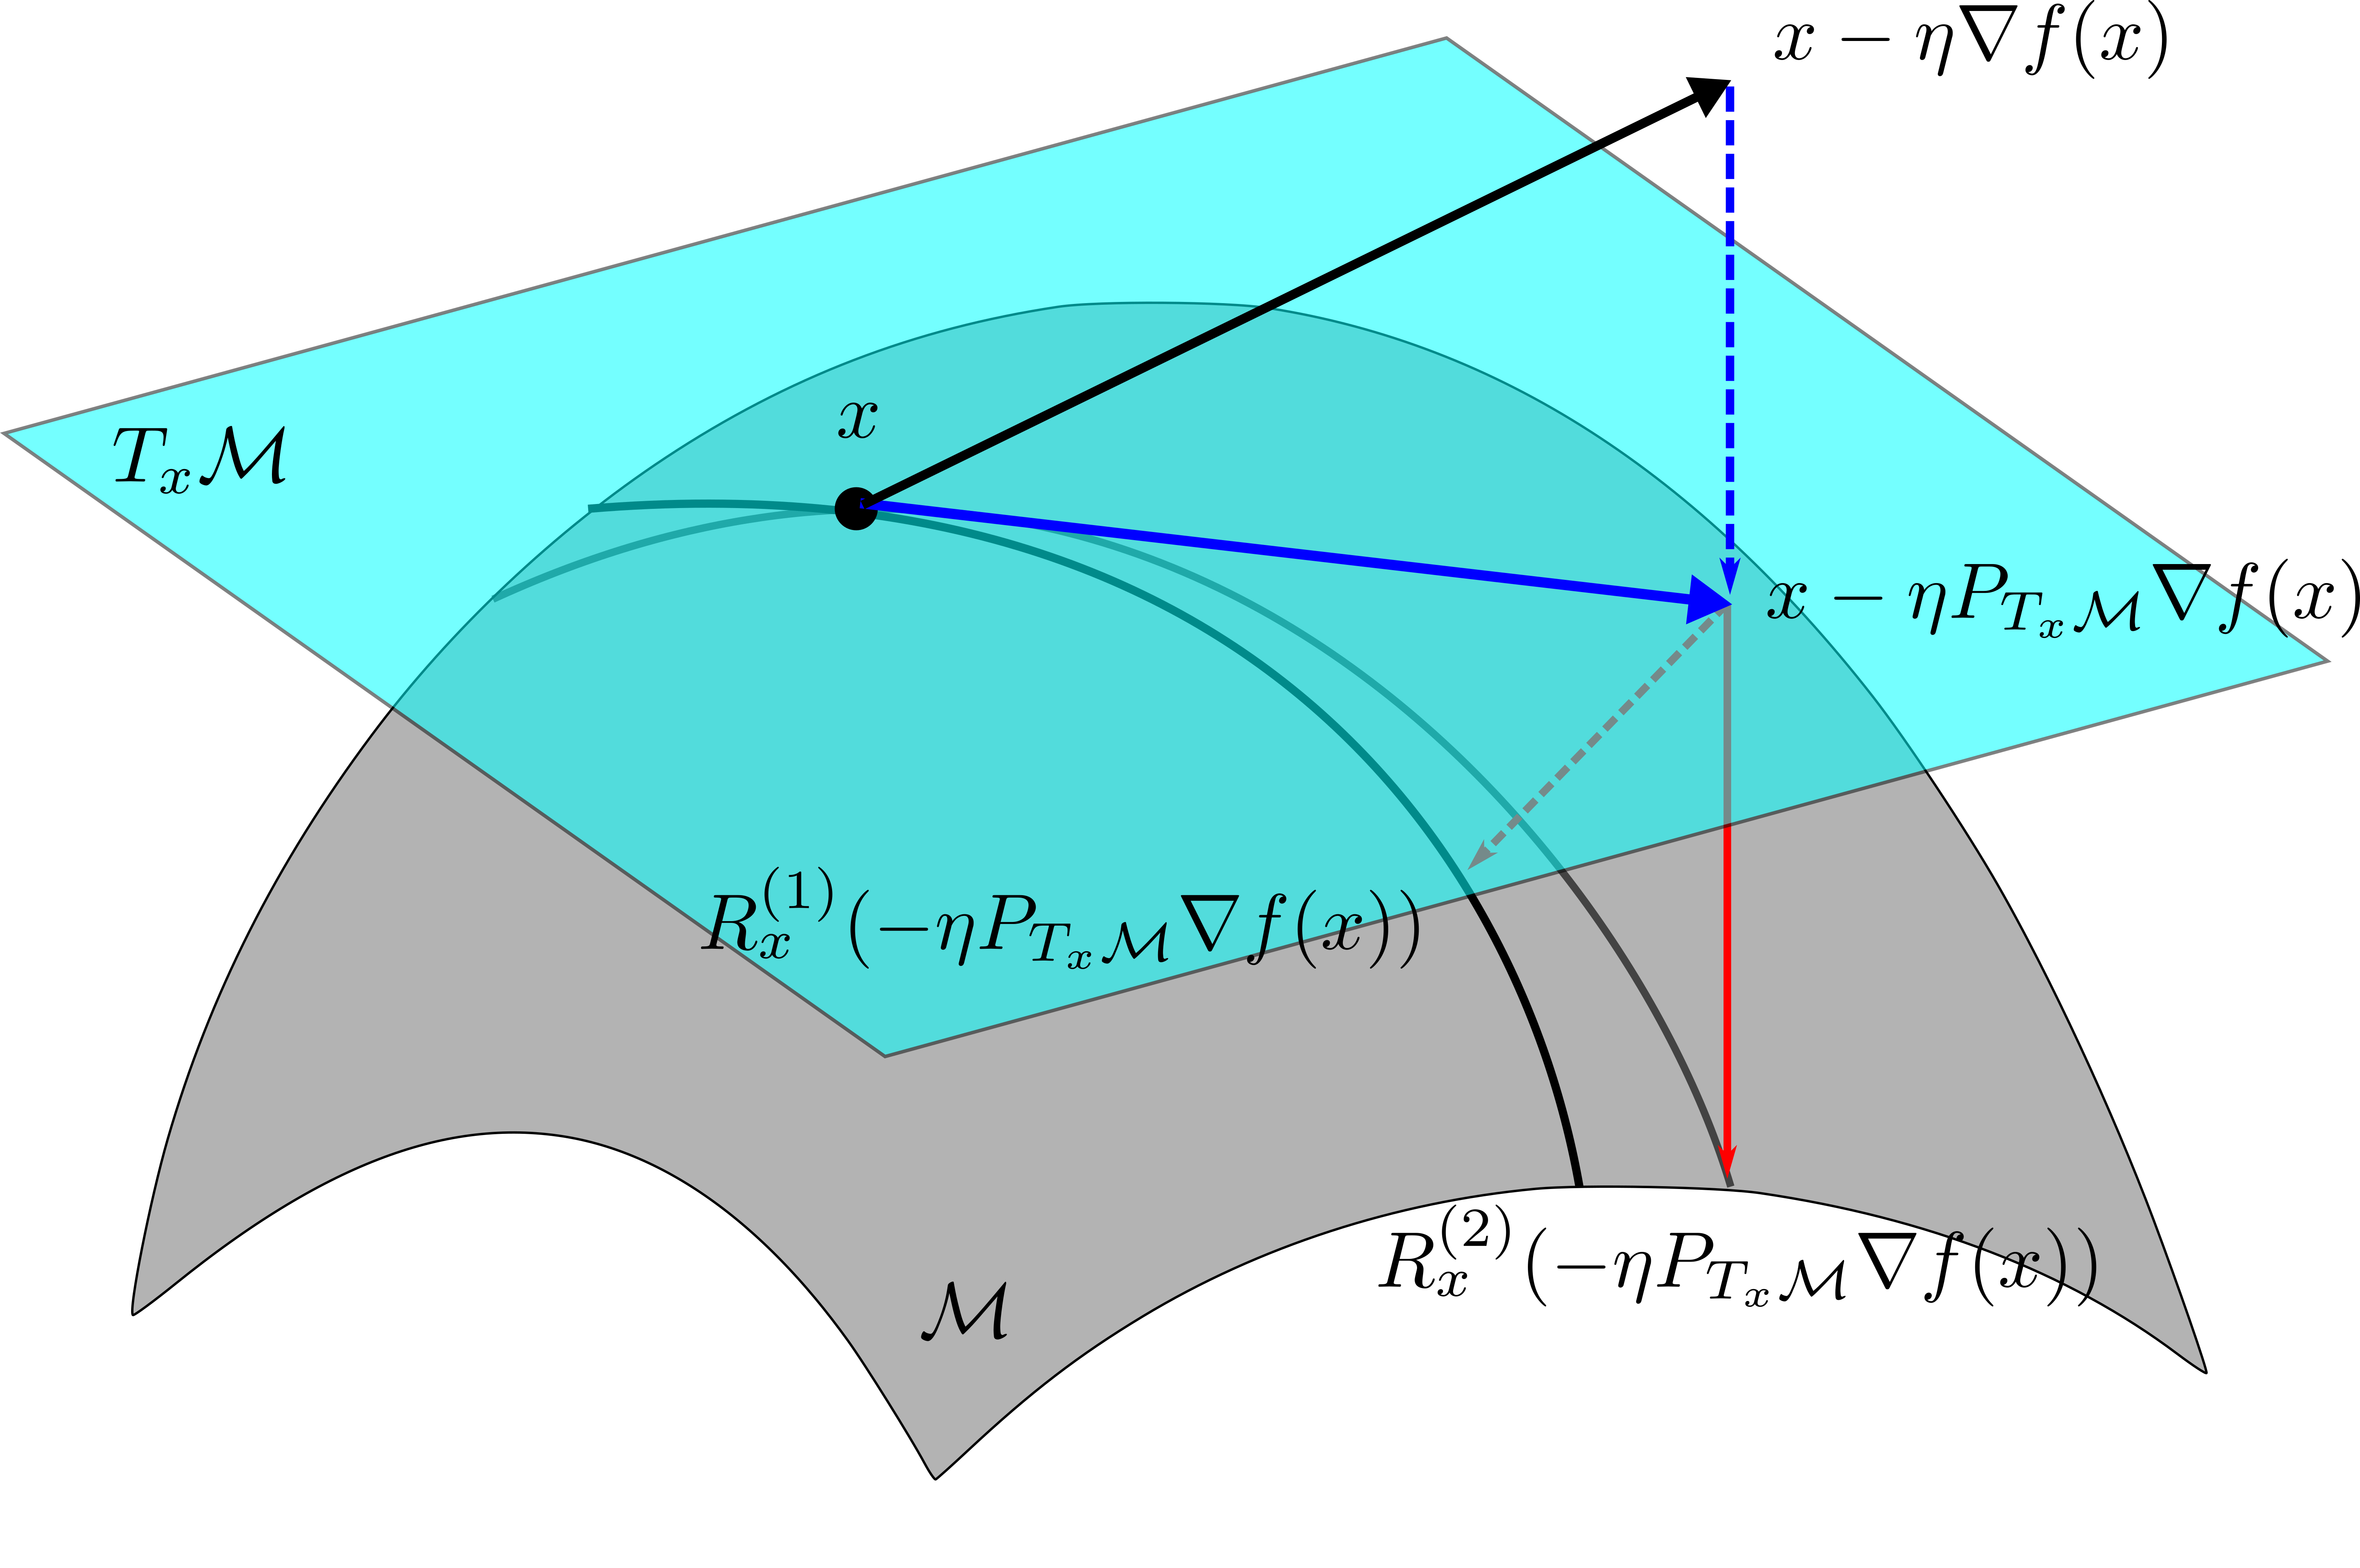
\includegraphics[width=0.8\textwidth]{figure/drawing} 
\par\end{centering}
\caption{The visualization of gradient descent algorithms on the manifold $\mathcal{M}$.
The black solid line is the Euclidean gradient. The blue solid line
is the projection of the Euclidean gradient to the tangent space.
The red solid line represents the orthographic retraction, while the
red dashed line represents the projective retraction.}
\label{fig:visualization} 
\end{figure}


\subsection{The geometry of the manifold of low-rank matrices}

\label{sec:geometry} To apply the gradient descent algorithm in Section~\ref{sec:background}
to the manifold of the low-rank matrices, the projection $P_{T_{x}\calM}$
and the retraction $R_{x}$ need to be defined. In this section, we
let $\calM$ be the manifold of all $\reals^{n_{1}\times n_{2}}$
matrices with rank $r$ and $\bX\in\calM$ be a matrix of rank $r$
and will find the explicit expressions of $P_{T_{x}\calM}$ and $R_{x}$.

The tangent space $T_{\bX}\calM$ and the retraction $R_{\bX}$ of
the manifold of the low-rank matrices have been well-studied~\cite{Absil2015}:
Assume that the SVD decomposition of $\bX$ is $\bX=\bU\bSigma\bV^{T}$,
then the tangent space $T_{\bX}\calM$ can be defined by $T_{\bX}\calM=\{\bA\bV\bV^{T}+\bU\bU^{T}\bB:\text{for}\,\,\bA\in\reals^{n_{1}\times n_{1}},\bB\in\reals^{n_{2}\times n_{2}}\}$
according to \cite{Absil2015}. The explicit formula for the projection
$P_{T_{\bX}\calM}$ is given in \cite[(9)]{Absil2015}: 
\begin{equation}
P_{T_{\bX}\calM}(\bD)=\bU\bU^{T}\bD+\bD\bV\bV^{T}-\bU\bU^{T}\bD\bV\bV^{T},\qquad\bD\in\reals^{n_{1}\times n_{2}}.\label{eq:projection}
\end{equation}
For completeness, a proof of \eqref{eq:projection} is presented in
Appendix.

There are various ways of defining retractions for the manifold of
low-rank matrices, and we refer the reader to~\cite{Absil2015} for
more details. In this work, we consider two types of retractions.
One is called the \textit{projective} retraction \cite{Shalit:2012:OLE:2503308.2188399,Vandereycken2013},
Given any $\bd\in T_{\bX}\calM$, the retraction is defined as the
nearest low-rank matrix to $\bX+\bd$ in terms of Frobenius norm:
\begin{equation}
R_{\bX}^{(1)}(\bd)=\argmin_{\bZ\in\calM}\|\bX+\bd-\bZ\|_{F}.\label{eq:projective}
\end{equation}
The solution is the rank-$r$ approximation of $\bX+\bd$ (for any
matrix $\bW$, its rank-$r$ approximation is given by $\sum_{i=1}^{r}\sigma_{i}\bu_{i}\bv_{i}^{T}$,
where $\sigma_{i},\bu_{i},\bv_{i}$ are the ordered singular values
and vectors of $\bW$).

In order to further improve computation efficiency, we also consider
the \textit{orthographic} retraction \cite{Absil2015}. Denoted by
$R_{\bX}^{(2)}(\bd)$, it is the nearest rank-$r$ matrix to $\bX+\bd$
that their difference is orthogonal to the tangent space $T_{\bX}\calM$:
\begin{align}
 & R_{\bX}^{(2)}(\bd)=\argmin_{\bZ\in\calM}\|\bX+\bd-\bZ\|_{F},\,\,\,\text{s.t. }\langle R_{\bX}^{(2)}(\bd)-(\bX+\bd),\bZ\rangle_{F}=0\,\,\text{for all \ensuremath{\bZ\in T_{\bX}\calM}},\label{eq:projective2}
\end{align}
and its explicit solution of \eqref{eq:projective2} is given in \cite[Section 3.2]{Absil2015},
\begin{equation}
R_{\bX}^{(2)}(\bd)=(\bX+\bd)\bV[\bU^{T}(\bX+\bd)\bV]^{-1}\bU^{T}(\bX+\bd),\label{eq:ortho_retraction}
\end{equation}
and a proof is given in Appendix. %The benefit of this retraction is that it has a simple explicit formula and there is no need to calculate singular value decomposition as the projective retraction.

\subsection{Derivation of the proposed algorithms}

\subsubsection{Derivation of Algorithm 1}

\label{sec:derivation1} The gradient descent algorithm \eqref{eq:gradient_manifold}
for solving \eqref{eq:objective} can be written as 
\begin{equation}
\bL^{(k+1)}=R_{\bL^{(k)}}(-\eta P_{T_{\bL^{(k)}}}\grad f(\bL^{(k)})),\label{eq:gradient}
\end{equation}
where $P_{T_{\bL^{(k)}}}$ is defined in \eqref{eq:projection} and
$R_{\bL^{(k)}}$ is defined in \eqref{eq:projective} or \eqref{eq:ortho_retraction}.
To derive the explicit algorithm, it remains to find the gradient
$\grad f$.

If the absolute values of all entries of $\bA$ are different, then
we have 
\begin{equation}
\grad f(\bL)=F(\bL-\bY).\label{eq:derivative}
\end{equation}
The proof of \eqref{eq:derivative} is deferred to Appendix. When
some entries of $\bA$ are equivalent and there is a tie in generating
$F(\bL-\bY)$, the objective function could be non-differentiable.
However, it can be shown that by arbitrarily breaking the tie, $F(\bL-\bY)$
is a subgradient of $f(\bL)$.

The corresponding gradient descent method (or subgradient method when
$f$ is not differentiable) with projective retraction can be written
as follows:
\begin{equation}
\bL^{(k+1)}\coloneqq\text{rank-\ensuremath{r} approximation of }\left[\bL^{(k)}-\eta P_{T_{\bL^{(k)}}}F(\bL^{(k)}-\bY)\right],\label{eq:alg_projective}
\end{equation}
where the rank-$r$ approximation has been defined after \eqref{eq:projective}.
This leads to Algorithm~\ref{alg:gradient} with Option 1.

For the orthographic retraction, i.e., $R_{\bL^{(k)}}$ defined according
to \eqref{eq:ortho_retraction}, by writing $\bD=F(\bL^{(k)}-\bY)$,
the update formula \eqref{eq:gradient} can be simplified to 
\begin{equation}
\bL^{(k+1)}\coloneqq(\bL^{(k)}-\eta\bD)\bV^{(k)}[\bU^{(k)T}(\bL^{(k)}-\eta\bD)\bV^{(k)}]^{-1}\bU^{(k)T}(\bL^{(k)}-\eta\bD),\label{eq:ortho_retraction1}
\end{equation}
where $\bU^{(k)}\in\reals^{n_{1}\times r}$ is any matrix such that
its column space is the same as the column space of $\bL^{(k)}$;
and $\bV^{(k)}\in\reals^{n_{2}\times r}$ is any matrix such that
its column space is the same as the row space of $\bL^{(k)}$. The
derivation of \eqref{eq:ortho_retraction1} is deferred to Appendix,
and it can be shown that the implementation of \eqref{eq:ortho_retraction1}
leads to Algorithm~\ref{alg:gradient} with Option 2. %It can be shown that both algorithms have a complexity of $O(n_1n_2r)$ per iteration, but empirically the gradient descent with the orthographic retraction is faster since it does not need to compute the singular value decomposition of $\bL^{(k)}$ in each iteration.

\subsubsection{Derivation of Algorithm 2}

\label{sec:partial} By a similar argument as in the previous section,
we can conclude that when all entries of $|\bL-\bY|$ are different
from each other, then applying the same procedure of deriving \eqref{eq:derivative},
we have 
\[
\grad\tilde{f}(\bL)=\tilde{F}(\bL-\bY);
\]
and $\tilde{F}(\bL-\bY)$ is a subgradient when $\tilde{f}(\bL)$
is not differentiable. Based on this observation, the algorithm under
the partially observed setting is identical to \eqref{eq:alg_projective}
or \eqref{eq:ortho_retraction1}, with $F$ replaced by $\tilde{F}$.
This gives the implementation of Algorithm 2.

\subsubsection{Basic convergence properties of Algorithms~\ref{alg:gradient} and~\ref{alg:gradient2}}

An interesting topic is that, can we still expect the algorithm to
have reasonable basic properties, such as convergence to a critical
point? Unfortunately, it is impossible to have such a theoretical
guarantee if a fixed step size $\eta$ is chosen: in general, the
subgradient method with fixed step size does not have the convergence
guarantee if the objective function is non-differentiable. However,
if we choose step size with line search, then any accumulation point
of $\bL^{(k)}$, $\widehat{\bL}$, would have the property that either
the objective function is not differentiable at $\widehat{\bL}$,
or it is a critical point in the sense that its Riemannian gradient
is zero. For example, the line search strategy for Algorithm~\ref{alg:gradient}
can be described as follows: start the step size $\eta_{k}$ with
a relatively large value, and repeatedly shrinks it by a factor of
$\beta\in(0,1)$ such that the following condition is satisfied: for
$\bL^{(k+1)}=R_{\bL^{(k)}}(-\eta_{k}P_{T_{\bL^{(k)}}}\grad f(\bL^{(k)}))$,
\[
f(\bL^{(k)})-f(\bL^{(k+1)})>c\eta_{k}\|P_{T_{\bL^{(k)}}}\grad f(\bL^{(k)})\|^{2},
\]
where $c\in(0,1)$ is prespecified. The argument for convergence follows
from the same argument as the proof of \cite[Theorem 4.3.1]{absil2009optimization}. 

\subsection{Prior works on manifold optimization}

The idea of optimization on manifolds has been well investigated in
the literature \cite{Vandereycken2013,Shalit:2012:OLE:2503308.2188399,absil2009optimization}.
For example, Absil et al. \cite{absil2009optimization} give a summary
of many advances in the field of optimization on manifolds. Manifold
optimization has been applied to many matrix estimation problems,
including recovering a low rank matrix from its partial entries, i.e.,
matrix completion \cite{5466511,Vandereycken2013,doi:10.1137/15M1050525}
and robust matrix completion in \cite{doi:10.1137/15M1025153}. In
fact, the problem studied in this work can be reformulated to the
problem analyzed in \cite{doi:10.1137/15M1025153}. In comparison,
our work studies a different algorithm and gives additional theoretical
guarantees.

In another aspect, while \cite{doi:10.1137/15M1050525} studies matrix
completion, it shares some similarities with this work: both works
study manifold optimization algorithms and have theoretical guarantees
showing that the proposed algorithms can recover the underlying low-rank
matrix exactly. In fact, \cite{doi:10.1137/15M1050525} can be considered
as our problem under the partially observed setting, without corruption
$\bS^{*}$. It proposes to solve 
\[
\argmin_{\bL\in\reals^{n_{1}\times n_{2}},\rank(\bL)=r}\sum_{(i,j)\in\Phi}(\bY_{ij}-\bL_{ij})^{2},
\]
which can be considered as $\tilde{f}$ in \eqref{eq:objective2}
when $\gamma=0$. %This work gives theoretical guarantees that the manifold gradient descent and conjugate gradient descent algorithms can recover the underlying low-rank matrix exactly. %One difference is that in this paper, $\Phi$ is a set chosen according to a probabilistic model; while our paper assume that it is a deterministic set.

\section{Theoretical Analysis}

\label{sec:theory} In this section, we analyze the theoretical properties
of Algorithms~\ref{alg:gradient} and~\ref{alg:gradient2} and compare
them with previous algorithms. Since the goal is to recover the low-rank
matrix $\bL^{*}$ and the sparse matrix $\bS^{*}$ from $\bY=\bL^{*}+\bS^{*}$,
to avoid identifiability issues, we need to assume that $\bL^{*}$
can not be both low-rank and sparse. Specifically, we make the following
standard assumptions on $\bL^{*}$ and $\bS^{*}$: 
\begin{assumption}
Each row of $\bS^{*}$ contains at most $\gamma^{*}n_{2}$ nonzero
entries and each column of $\bS^{*}$ contains at most $\gamma^{*}n_{1}$
nonzero entries. In other words, for $\gamma^{*}\in[0,1)$, assume
$\bS^{*}\in\mathcal{S}_{\gamma^{*}}$ where 
\begin{equation}
\mathcal{S_{\gamma^{*}}\coloneqq}\left\{ A\in\mathbb{R}^{n_{1}\times n_{2}}\mid\|A_{i,\cdot}\|_{0}\leq\gamma^{*}n_{2},\ \mathrm{for}\ 1\leq i\leq n_{1};\|A_{\cdot,j}\|_{0}\leq\gamma^{*}n_{1},\ \mathrm{for}\ 1\leq j\leq n_{2}\right\} .\label{eq:ass1}
\end{equation}
\end{assumption}
%
\begin{assumption}
The low-rank matrix $\bL^{*}$ is not near-sparse. To achieve this,
we require that $\bL^{*}$ must be $\mu$-coherent. Given the singular
value decomposition (SVD) $\bL^{*}=\bU^{*}\bSigma^{*}\bV^{*T}$, where
$\bU^{*}\in\reals^{n_{1}\times r}$ and $\bV^{*}\in\reals^{n_{2}\times r}$,
we assume there exists an incoherence parameter $\mu$ such that 
\begin{equation}
\|\bU^{*}\|_{2,\infty}\leq\sqrt{\frac{\mu r}{n_{1}}},\,\,\,\|\bV^{*}\|_{2,\infty}\leq\sqrt{\frac{\mu r}{n_{2}}},\label{eq:ass2}
\end{equation}
where the norm $\|\cdot\|_{2,\infty}$ is defined by $\|\bA\|_{2,\infty}=\max_{\|\bz\|_{2}=1}\|\bA\bz\|_{\infty}$
and $\|\bx\|_{\infty}=\max_{i}|\bx_{i}|$. 
\end{assumption}

\subsection{Analysis of Algorithm~\ref{alg:gradient}}

With Assumption 1 and 2, we have the following theoretical results
regarding the convergence rate, initialization, and stability of Algorithm~\ref{alg:gradient}:
\begin{theorem}[Linear convergence rate, fully observed case]
\label{thm:main} Suppose that $\|\bL^{(0)}-\bL^{*}\|_{F}\leq a\sigma_{r}(\bL^{*})$,
where $\sigma_{r}(\bL^{*})$ is the $r$-th largest singular value
of $\bL^{*}$, $a\leq1/2$, $\gamma>2\gamma^{*}$ and $C_{1}=\sqrt{4(\gamma+2\gamma^{*})\mu r+4\frac{\gamma^{*}}{\gamma-\gamma^{*}}+a^{2}}<\frac{1}{2}$,
then there exists $\eta_{0}=\eta_{0}(C_{1},a)>0$ that does not depend
on $k$, such that for all $\eta\leq\eta_{0}$, 
\[
\|\bL^{(k)}-\bL^{*}\|_{F}\leq\Big(1-\frac{1-2C_{1}}{8}\eta\Big)^{k}\|\bL^{(0)}-\bL^{*}\|_{F}.
\]
\end{theorem}
\begin{remark}
(Choices of parameters). It is shown in the proof that $\eta_{0}$
can be set to the solution of the equation 
\[
\eta_{0}(1+C_{1})^{2}\left[\frac{1}{2}+\frac{a^{2}}{1-\eta_{0}(1+C_{1})a}\right]=\frac{1}{8}(1-2C_{1}).
\]
Since the LHS is an increasing function of $\eta_{0}$ and is zero
when $\eta_{0}=0$, and its RHS is a positive number.

While $C_{1}<1/2$ requires $\sqrt{4\gamma^{*}/(\gamma-\gamma^{*})}<1/2$,
i.e., $\gamma>17\gamma^{*}$. In practice a much smaller $\gamma$
can be used. In Section~\ref{sec:simu}, $\gamma=1.5\gamma^{*}$
is used and works well for a large number of examples. It suggests
that some constants in Theorem~\ref{thm:main} might be due to the
technicalities in the proof and can be potentially improved. 
\end{remark}
%
\begin{remark}
(Simplified choices of parameters) There exists $c_{1}$ and $c_{2}$
such that if $a<c_{1}$, $\gamma^{*}\mu r<c_{2}$ and $\gamma=65\gamma^{*}$,
then one can choose $\eta_{0}=1/8$. In this sense, if the initialization
of the algorithm is good, then the algorithm can handle $\gamma^{*}$
as large as $O(1/\mu r)$. In addition, it requires $O(\log(1/\epsilon))$
iterations to achieve $\|\bL^{(k)}-\bL^{*}\|_{F}/\|\bL^{(0)}-\bL^{*}\|_{F}<\epsilon$. 
\end{remark}
Since the statements require proper initializations (i.e., small $a$),
the question arises as to how to choose proper initializations. The
work by \cite{DBLP:conf/nips/YiPCC16} shows that if the rank-$r$
approximation to $F(\bY)$ is used as the initialization $\bL^{(0)}$,
then such initialization has the upper bound $\|\bL^{(0)}-\bL^{*}\|$
according to the proofs of \cite[Theorems 1 and 3]{DBLP:conf/nips/YiPCC16}
(we borrow this estimation along with the fact that $\|\bL^{(0)}-\bL^{*}\|_{F}\leq\sqrt{2r}\|\bL^{(0)}-\bL^{*}\|$). 
\begin{theorem}[Initialization, fully observed case]
\label{thm:initialization} If $\gamma>\gamma^{*}$ and we initialize
$\bL^{(0)}$ using the rank-$r$ approximation to $F(\bY)$, then
\[
\|\bL^{(0)}-\bL^{*}\|_{F}\leq8\gamma\mu r\sqrt{2r}\sigma_{1}(\bL^{*}).
\]
\end{theorem}
The combination of Theorem~\ref{thm:main}, \ref{thm:initialization}
and the fact that $\gamma=O(\gamma^{*})$ implies that under the fully
observed setting, the tolerance of the proposed algorithms to corruption
is at most $\gamma^{*}=O(\frac{1}{\mu r\sqrt{r}\kappa})$, where $\kappa=\sigma_{1}(\bL^{*})/\sigma_{r}(\bL^{*})$
is the condition number of $\bL^{*}$. We also study the stability
of Algorithm~\ref{thm:main} in the following statement. 
\begin{theorem}[Stability, fully observed case]
\label{thm:noisy} Let $\bL$ be the current value, and let $\bL^{+}$
be the next update by applying Algorithm~\ref{alg:gradient} to $\bL$
for one iteration. Assuming $\bY=\bL^{*}+\bS^{*}+\bN^{*}$, where
$\bN^{*}$ is a random Gaussian noise i.i.d. sampled from $N(0,\sigma^{2})$,
$\gamma>10\gamma^{*}$ and $(\gamma+2\gamma^{*})\mu r<1/64$, then
there exist $C,a,c,\eta_{0}>0$ such that when $\eta<\eta_{0}$, 
\begin{equation}
P\left(\|\bL^{+}-\bL^{*}\|_{F}\leq\left(1-c\eta\right)\|\bL-\bL^{*}\|_{F}\,\,\mathrm{for}\ \mathrm{all}\ \bL\in\Gamma\right){\rightarrow}1,\quad\mathrm{as}\ n_{1},n_{2}\rightarrow\infty,\label{eq:prob}
\end{equation}
where 
\[
\Gamma=\{\bL\in\reals^{n_{1}\times n_{2}}:\rank(\bL)=r,C\sigma\sqrt{(n_{1}+n_{2})r\ln(n_{1}n_{2})}\leq\|\bL-\bL^{*}\|_{F}\leq a\sigma_{r}(\bL^{*})\|,
\]
\end{theorem}
Since $1-c\eta<1$, and Theorem \ref{thm:noisy} shows that when the
observation $\bY$ is contaminated with a random Gaussian noise, if
$\bL^{(0)}$ is properly initialized such that $\|\bL^{(0)}-\bL^{*}\|_{F}<a\sigma_{r}(\bL^{*})$,
Algorithms~\ref{alg:gradient} will converge to a neighborhood of
$\bL^{*}$ given by 
\[
\{\bL:\|\bL-\bL^{*}\|_{F}\leq C\sigma\sqrt{(n_{1}+n_{2})r\ln(n_{1}n_{2})}\}
\]
in $[-\log(\|\bL^{(0)}-\bL^{*}\|_{F})+\log(C\sigma\sqrt{(n_{1}+n_{2})r\ln(n_{1}n_{2})})]/\log(1-c\eta)$
iterations, with probability goes to $1$ as $n_{1},n_{2}\rightarrow\infty$.

\subsection{Analysis of Algorithm~\ref{alg:gradient2}}

For the partially observed setting, we assume that each entry of $\bY=\bL^{*}+\bS^{*}$
is observed with probability $p$. That is, for any $1\leq i\leq n_{1}$
and $1\leq j\leq n_{2}$, $\Pr((i,j)\in\mathbf{\Phi})=p$. Then we
have the following statement on convergence: 
\begin{theorem}[Linear convergence rate, partially observed case]
\label{thm:main2} There exists $c>0$ such that for $n=\max(n_{1},n_{2})$,
if $p\geq\max(c\mu r\log(n)/\epsilon^{2}\min(n_{1},n_{2}),\frac{56}{3}\frac{\log n}{\gamma\min(n_{1},n_{2})})$,
then with probability $1-2n^{-3}-6n^{-1}$, 
\begin{align}
\frac{\|\bL^{(k)}-\bL^{*}\|_{F}}{\|\bL^{(0)}-\bL^{*}\|_{F}}\leq & \Big[\sqrt{1-p^{2}(1-\epsilon)^{2}\left(2\eta\left(1-\tilde{C}_{1}-\frac{ap(1+\epsilon)}{2(1-a)}(1+\tilde{C}_{1})\right)-\eta^{2}(1+\tilde{C}_{1})^{2}\right)}\nonumber \\
+ & \frac{\eta^{2}a^{2}(p+p\epsilon)^{2}(1+\tilde{C}_{1})^{2}}{1-\eta a(p+p\epsilon)(1+\tilde{C}_{1})}\Big]^{k}\label{eq:main2}
\end{align}
for 
\[
\tilde{C}_{1}=\frac{1}{p(1-\epsilon)}\Big[6(\gamma+2\gamma^{*})p\mu r+4\frac{3\gamma^{*}}{\gamma-3\gamma^{*}}(\sqrt{p(1+\epsilon)}+\frac{a}{2})^{2}+a^{2}\Big].
\]
\end{theorem}
\begin{remark}
(Choice of parameters) Note that when $\eta$ is small, the RHS of
\eqref{eq:main2} is in the order of 
\[
1-p^{2}(1-\epsilon)^{2}\left(1-\tilde{C}_{1}-\frac{ap(1+\epsilon)}{2(1-a)}(1+\tilde{C}_{1})\right)\eta+O(\eta^{2}).
\]
As a result, to make sure that the RHS of \eqref{eq:main2} to be
smaller than $1$ for small $\eta$, we assume that 
\begin{equation}
1-\tilde{C}_{1}-\frac{ap(1+\epsilon)}{2(1-a)}(1+\tilde{C}_{1})>0.\label{eq:requirement}
\end{equation}
For example, when ${ap(1+\epsilon)}={4(1-a)}$, it requires that $\tilde{C}_{1}<1/3$.
If \eqref{eq:requirement} holds, then there exists $\eta_{0}=\eta_{0}(\tilde{C}_{1},p,\epsilon,a)$
such that for all $\eta\leq\eta_{0}$, the RHS of \eqref{eq:main2}
is smaller than $1$.

The practical choices of $\eta$ and $\gamma$ will be discussed in
Section~\ref{sec:simu}. 
\end{remark}
%
\begin{remark}
(Simplified choice of parameters) There exists $\{c_{i}\}_{i=1}^{4}>0$
such that when $\epsilon<1/2$, $a<c_{1}p$, $\gamma^{*}\mu r<c_{2}$
and $\gamma=c_{3}\gamma^{*}$, then when $\eta<1/8$, 
\[
\frac{\|\bL^{(k)}-\bL^{*}\|_{F}}{\|\bL^{(0)}-\bL^{*}\|_{F}}\leq(1-c_{4}\eta p^{2})^{k}.
\]
Compared with the result in Theorem~\ref{thm:main}, the addition
parameter $p$ appears in both the initialization requirement $a<c_{1}p$
as well as the convergence rate. This makes the result weaker, but
we suspect that the dependence on the subsampling ratio $p$ could
be improved through a better estimation in \eqref{eq:aa} and the
estimation of $\tilde{C}_{1}$ in Lemma~\ref{lemma:bD2}, and we
leave it as a possible future direction. 
\end{remark}
We present a method of obtaining a proper initialization in Theorem
\ref{thm:initialization2}. Combining it with Theorem~\ref{thm:main2},
Algorithm~\ref{alg:gradient2} allows the corruption level $\gamma^{*}$
to be in the order of $O(\frac{p}{\mu r\sqrt{r}\kappa})$.
\begin{theorem}[Initialization, partially observed case]
\label{thm:initialization2} There exists $c_{1},c_{2},c_{3}>0$
such that if $\gamma>2\gamma^{*}$, and $p\geq c_{2}(\frac{\mu r^{2}}{\epsilon^{2}}+\frac{1}{\alpha})\log n/\min(n_{1},n_{2})$,
and we initialize $\bL^{(0)}$ using the rank-$r$ approximation to
$F(\bY)$, then 
\[
\|\bL^{(0)}-\bL^{*}\|_{F}\leq16\gamma\mu r\sigma_{1}(\bL^{*})\sqrt{2r}+2\sqrt{2}c_{1}\epsilon\sigma_{1}(\bL^{*})
\]
with probability at least $1-c_{3}n^{-1}$, where $\sigma_{1}(\bL^{*})$
is the largest singular value of $\bL^{*}$ .
\end{theorem}

\subsection{Comparison with Alternating Gradient Descent}

\label{sec:compare} Since our objective functions are equivalent
to the objective functions of the alternating gradient descent (AGD)
in \cite{DBLP:conf/nips/YiPCC16}, it would be interesting to compare
these two works. The only difference of these two works lies in the
algorithmic implementation: our methods use the gradient descent on
the manifold of low-rank matrices, while the methods in \cite{DBLP:conf/nips/YiPCC16}
use alternating gradient descent on the factors of the low-rank matrix.
In the following we compare the results of both works from four aspects: 
\begin{enumerate}
\item \textbf{Accuracy of initialization.} What is the largest value $t$
that the algorithm can tolerate, such that for any initialization
$\bL^{(0)}$ satisfying $\|\bL^{(0)}-\bL^{*}\|_{F}\leq t$, the algorithm
is guaranteed to converge to $\bL^{*}$?
\item \textbf{Convergence rate.} What is the smallest number of iteration
steps $k$ such that the algorithm reaches a given convergence criterion
$\epsilon$, i.e. $\|\bL^{(k)}-\bL^{*}\|_{F}/\|\bL^{(0)}-\bL^{*}\|_{F}<\epsilon$?
\item \textbf{Corruption level (perfect initialization).} Suppose that the
initialization is in a sufficiently small neighborhood of $\bL^{*}$
(i.e. there exists a very small $\epsilon_{0}>0$ such that $\bL^{(0)}$
satisfies $\|\bL^{(0)}-\bL^{*}\|_{F}<\epsilon_{0}$), what is the
maximum corruption level that can be tolerated in the convergence
analysis?
\item \textbf{Corruption level (proper initialization).} Suppose that the
initialization is given by the procedure in Theorem~\ref{thm:initialization}
(for the partially observed case) and \ref{thm:initialization2} (for
the fully observed case), what is the maximum corruption level that
can be tolerated? 
\end{enumerate}
These comparisons are summarized in Table~\ref{tab:compare}. We
can see that under the full observed setting, our results remove or
reduce the dependence on the condition number $\kappa$, while keeping
other values unchanged. Under the partially observed setting our results
still have the advantage of less dependence on $\kappa$, but sometimes
require an additional dependence on the subsampling ratio $p$. The
simulation results discussed in the next section also verify that
when $\kappa$ is large our algorithms have better performance, while
that the slowing effect of $p$ under the partially observed setting
is not significant. As discussed after Theorem~\ref{thm:main2},
we suspect that this dependence could be removed after a more careful
analysis (or more assumptions).

\begin{table*}[htbp]
\centering %
\begin{tabular}{lllll}
\toprule 
\multirow{ 2}{*}{Criterion}  & {Accuracy of}  & Convergence  & Max corruption  & Max corruption \tabularnewline
 & initialization & rate  & (perfect init.)  & (proper init.) \tabularnewline
\midrule 
Algorithm 1  & $O(\sigma_{r}(\bL^{*}))$  & $O(\log(\frac{1}{\epsilon}))$  & $O(\frac{1}{\mu r})$  & $O(\frac{1}{\mu r^{1.5}\kappa})$\tabularnewline
APG (full)  & $O(\frac{\sigma_{r}(\bL^{*})}{\sqrt{\kappa}})$  & $O(\kappa\log(\frac{1}{\epsilon}))$  & $O(\frac{1}{\kappa^{2}\mu r})$  & $O(\frac{1}{\max(\mu r^{1.5}\kappa^{1.5},\kappa^{2}\mu r)})$\tabularnewline
Algorithm 2  & $O(\sqrt{p}\sigma_{r}(\bL^{*}))$  & $O(\log(\frac{1}{\epsilon})/p^{2})$  & $O(\frac{1}{\mu r})$  & $O(\frac{\sqrt{p}}{\mu r^{1.5}\kappa})$\tabularnewline
APG (partial)  & $O(\frac{\sigma_{r}(\bL^{*})}{\kappa})$  & $O(\kappa\mu r\log(\frac{1}{\epsilon})$  & $O(\frac{1}{\kappa^{2}\mu r})$  & $O(\frac{1}{\max(\mu r^{1.5}\kappa^{1.5},\kappa^{2}\mu r)})$\tabularnewline
\bottomrule
\end{tabular}

\caption{{\small{}{Comparison of the theoretical guarantees in our work and
the alternating gradient descent algorithm in \cite{DBLP:conf/nips/YiPCC16}.
The four criteria are explained in details in Section~\ref{sec:compare}.
\label{tab:compare}}}}
%\footnotesize
\end{table*}

Here we use a simple example to give some intuition of why our proposed
methods work better than gradient descent method based on factorization.
Let us consider the following simple optimization problem: 
\[
\argmin_{\bz\in\reals^{m}}f(\bz),\,\,\,\text{where \ensuremath{\bz=\bA\bx+\bB\by}},
\]
where $\bx,\by\in\reals^{n}$ and $\bA,\bB\in\reals^{m\times n}$.
In this example, $(\bx,\by)$ can be considered as the ``factors''
of $\bz$. The gradient descent method on the factors $(\bx,\by)$
is then given by 
\begin{equation}
\bx^{+}=\bx-\eta\bA^{T}f'(\bz),\,\,\,\by^{+}=\by-\eta\bB^{T}f'(\bz).\label{eq:factor}
\end{equation}
Writing the update formula \eqref{eq:factor} in terms of $\bz$,
it becomes 
\[
\bz^{+}=\bA\bx^{+}+\bB\by^{+}=\bz-\eta(\bA\bA^{T}+\bB\bB^{T})f'(\bz).
\]

As a result, the ``gradient descent on factors $(\bx,\by)$'' has
a direction of $-(\bA\bA^{T}+\bB\bB^{T})f'(\bz)$. In comparison,
the gradient descent on the variable $\bz$ has a direction of $-f'(\bz)$,
which is the direction that $f$ decreases fastest. If $\bA\bA^{T}+\bB\bB^{T}$
is a matrix with a large condition number, then we expect that the
gradient descent method on factors $(\bx,\by)$ would not work well.
This example shows that generally, compared to applying the gradient
descent method to the factors of a variable, it is better to apply
it to the variable itself. Similar to this example, our method applies
gradient descent on the $\bL$ itself while \cite{DBLP:conf/nips/YiPCC16}
applies gradient descent to the factors of $\bL$.

\subsection{Comparison with other robust PCA algorithms}

In this section we compare our result with other robust PCA methods
and summarize them in Table \ref{tab:compare2}. Some criterion in
Table \ref{tab:compare} are not included since they do not apply.
For example, \cite[Alternating Projection]{NIPS2014_5430} only analyzes
the algorithm with specific initialization, and the criterion 1 and
3 in Table \ref{tab:compare} do not apply to this work. As a result,
we only compare the maximum corruption ratio that these methods can
handle, and the computational complexity per iteration in Table \ref{tab:compare2}.
As for the convergence rate, it depends on assumptions on parameters
such as the coherence parameter, rank, and the size of the matrix:
The alternating projection~\cite{NIPS2014_5430} requires $10\log(4n_{1}\mu^{2}r\|\bY-\bL^{(0)}\|_{2}/\epsilon\sqrt{n_{1}n_{2}})$
iterations to achieve an accuracy $\epsilon$, under the assumptions
that $\gamma^{*}<1/512\mu r^{2}$ and a tuning parameter is chosen
to be $4\mu^{2}r\sqrt{n_{1}n_{2}}$. The alternating minimization
method~\cite{conf/aistats/GuWL16} have the guarantee that if $\|\bL^{(1)}-\bL^{*}\|_{2}\leq\sigma_{1}(\bL^{*})$,
then 
\[
\|\bL^{(k+1)}-\bL^{*}\|_{F}\leq\sigma_{1}\left(\frac{96\sqrt{2}\nu\mu\sqrt{r}(s^{*}/d)^{3/2}\kappa\sigma_{1}}{1-24\sqrt{2}\nu\mu\sqrt{r}(s^{*}/d)^{3/2}\kappa\sigma_{1}}\right)^{k}\|\bL^{(1)}-\bL^{*}\|_{F},
\]
where $\nu$ is a parameter concerning the coherence of $\bL^{*}$,
$s^{*}$ is the number of nonzero entries in $\bS^{*}$, $d=\min(n_{1},n_{2})$.
As a result $s^{*}/d$ is approximately $\gamma^{*}\max(n_{1},n_{2})$
in our notation. If $\nu$ is in the order of $O(1)$, then this results
requires that $\mu\sqrt{r}\kappa\sigma_{1}\max(n_{1},n_{2})^{3/2}\gamma^{*\,3/2}\leq O(1)$,
which is more restrictive than our assumption in Theorem~\ref{thm:main}
that $\gamma^{*}\mu r\leq O(1)$. Convex methods usually have convergence
rate guarantees based on convexity, for example, the accelerated proximal
gradient method \cite{Shen_anaccelerated} has a convergence rate
of $O(1/k^{2})$. While it is a slower convergence rate compared to
the result in Theorem~\ref{thm:main} in this work or the results
in~\cite{NIPS2014_5430,conf/aistats/GuWL16} and it does not necessarily
converge to the correct solution, this result does not depend on any
assumption on the low-rank matrix and the corruption ratio.

\begin{table*}[htbp]
\centering %
\begin{tabular}{lll}
\toprule 
\multirow{ 2}{*}{Criterion}  & Maximum  & Complexity \tabularnewline
 & corruption level & per iteration\tabularnewline
\midrule 
Algorithm~\ref{alg:gradient}  & $O(1/\kappa\mu r^{3/2})$ & $O(rn_{1}n_{2})$\tabularnewline
Convex methods  & $O(1/\mu^{2}r)$  & $O(n_{1}n_{2}\min(n_{1},n_{2}))$ \tabularnewline
\cite{NIPS2014_5430}  & ${1/512\mu^{2}r}$  & $O(r^{2}n_{1}n_{2})$ \tabularnewline
\cite{conf/aistats/GuWL16}  & $O(1/\mu^{2/3}r^{2/3}\min(n_{1},n_{2}))$  & $O(r^{2}n_{1}n_{2})$ \tabularnewline
\cite{DBLP:conf/nips/YiPCC16} & $O(1/\kappa^{2}\mu r^{3/2})$ & $O(rn_{1}n_{2})$ \tabularnewline
\bottomrule
\end{tabular}

\caption{{\small{}{Comparison of the theoretical guarantees in our work and
some other robust PCA algorithms. \label{tab:compare2}}}}
%\footnotesize
\end{table*}

The stability in Theorem~\ref{thm:noisy} is comparable to analysis
in \cite{NIPS2014_5430} (the works \cite{conf/aistats/GuWL16} and
\cite[Alternating Gradient Descent]{DBLP:conf/nips/YiPCC16} do not
have stability analysis). The work \cite{NIPS2014_5430} assumes that
$\|\bN^{*}\|_{\infty}<\sigma_{r}(\bL^{*})/100n_{2}$ and proves that
the output of their algorithm $\widehat{\bL}$ satisfies 
\[
\|\widehat{\bL}-\bL^{*}\|_{F}\leq\epsilon+2\mu^{2}r\left(7\|\bN^{*}\|_{2}+\frac{8\sqrt{n_{1}n_{2}}}{\sqrt{r}}\|\bN^{*}\|_{\infty}\right),
\]
where $\epsilon$ is the error of the algorithm when there is no noise.
If $\bN^{*}$ is i.i.d. sampled from $N(0,\sigma^{2})$, this result
suggests that $\|\widehat{\bL}-\bL^{*}\|_{F}$ is bounded above by
$\epsilon+O(\mu^{2}\sqrt{rn_{1}n_{2}}\sigma)$. In comparison, Theorem~\ref{thm:noisy}
suggests that after a few iterations, $\|{\bL}^{(k)}-\bL^{*}\|_{F}$
is bounded above by $C\sigma\sqrt{(n_{1}+n_{2})r\ln(n_{1}n_{2})}$
with high probability, which is a tighter upper bound.

\section{Simulations}

\label{sec:simu} In this section, we test the performance of the
proposed algorithms by simulated data sets and real data sets. The MATLAB implementation of our algorithm used in this section is available at \url{https://sciences.ucf.edu/math/tengz/}. For simulated data sets, we generate $\bL^{*}$ by $\bU\bSigma\bV^{T}$,
where $\bU\in\reals^{n_{1}\times r}$ and $\bV\in\reals^{n_{2}\times r}$
are random matrices that i.i.d. sampled from $N(0,1)$, and $\bSigma\in\reals^{n_{1}\times r}$
is an diagonal matrix. As for $\bS^{*}\in\reals^{n_{1}\times n_{2}}$,
each entry is sampled from $N(0,100)$ with probability $q$, and
is zero with probability $1-q$. That is, $q$ represents the level
of sparsity in the sparse matrix $\bS^{*}$. It measures the overall
corruption level of $\bY$ and is associated with the corruption level
$\gamma^{*}$ ($\gamma^{*}$ measures the row and column-wise corruption
level). For the partially observed case, we assume that each entry
of $\bY$ is observed with probability $p$.

\subsection{Choice of parameters}

\label{sec:simu1} We first investigate the performance of the proposed
algorithms, in particular, the dependence on the parameters $\eta$
and $\gamma$. In simulations, we let $[n_{1},n_{2}]=[500,600]$,
$r=3$, $\bSigma=\bI$, and $q=0.02$. For the partially observed
case, we let $p=0.2$. 

The first simulation investigates the following questions: 
\begin{itemize}
\item Should we use the Algorithms~\ref{alg:gradient} and~\ref{alg:gradient2}
with Option 1 or Option 2? 
\item What is the appropriate choice of the step size $\eta$? 
\end{itemize}
The simulation results for Option 1 an 2 with various step sizes are
visualized in Figure~\ref{fig:options}, which show that the two
options perform similarly. Usually the algorithms converge faster
when the step size is larger. However, if the step size is too large
then it might diverge. As a result, we use the step size $\eta=0.7$
for Algorithm~\ref{alg:gradient} and $0.7/p$ for Algorithm~\ref{alg:gradient2}
for the following simulations.

\begin{figure}
\centering 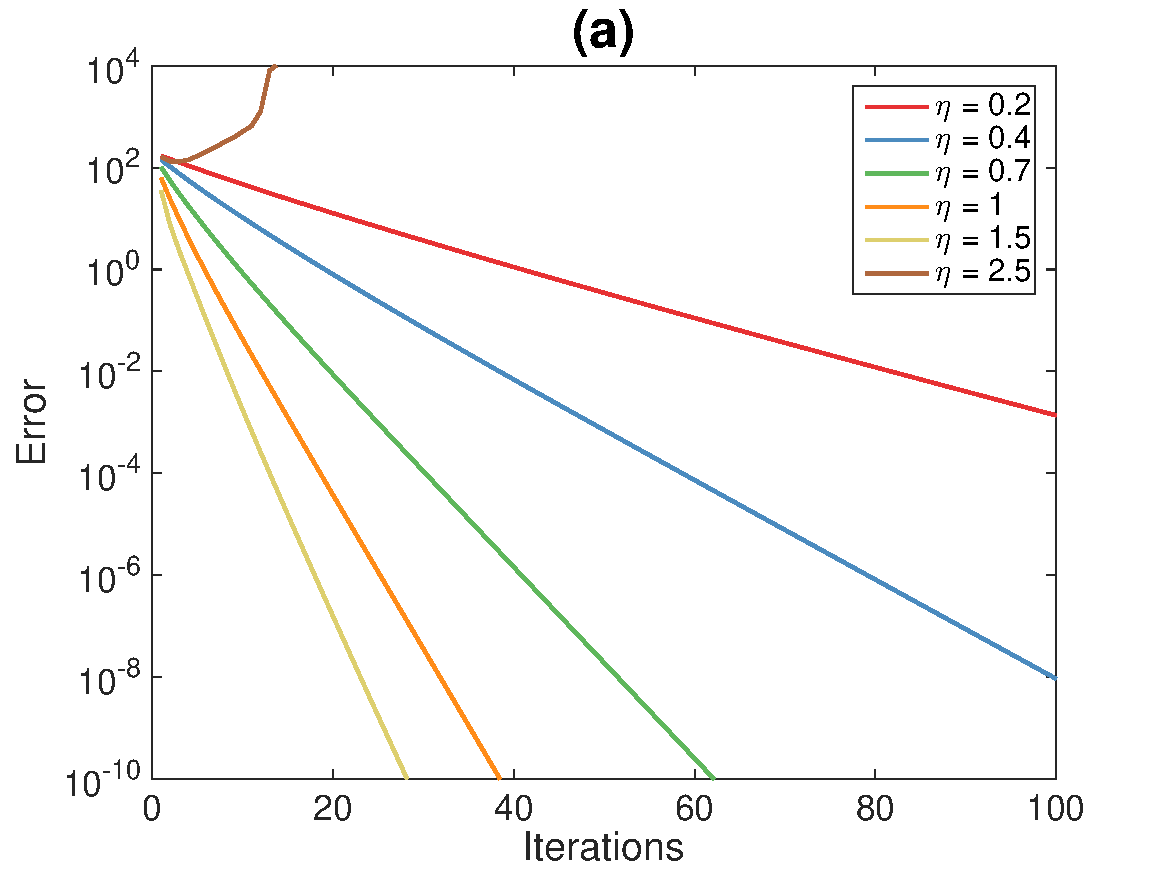
\includegraphics[width=0.49\textwidth]{figure/kappa12}
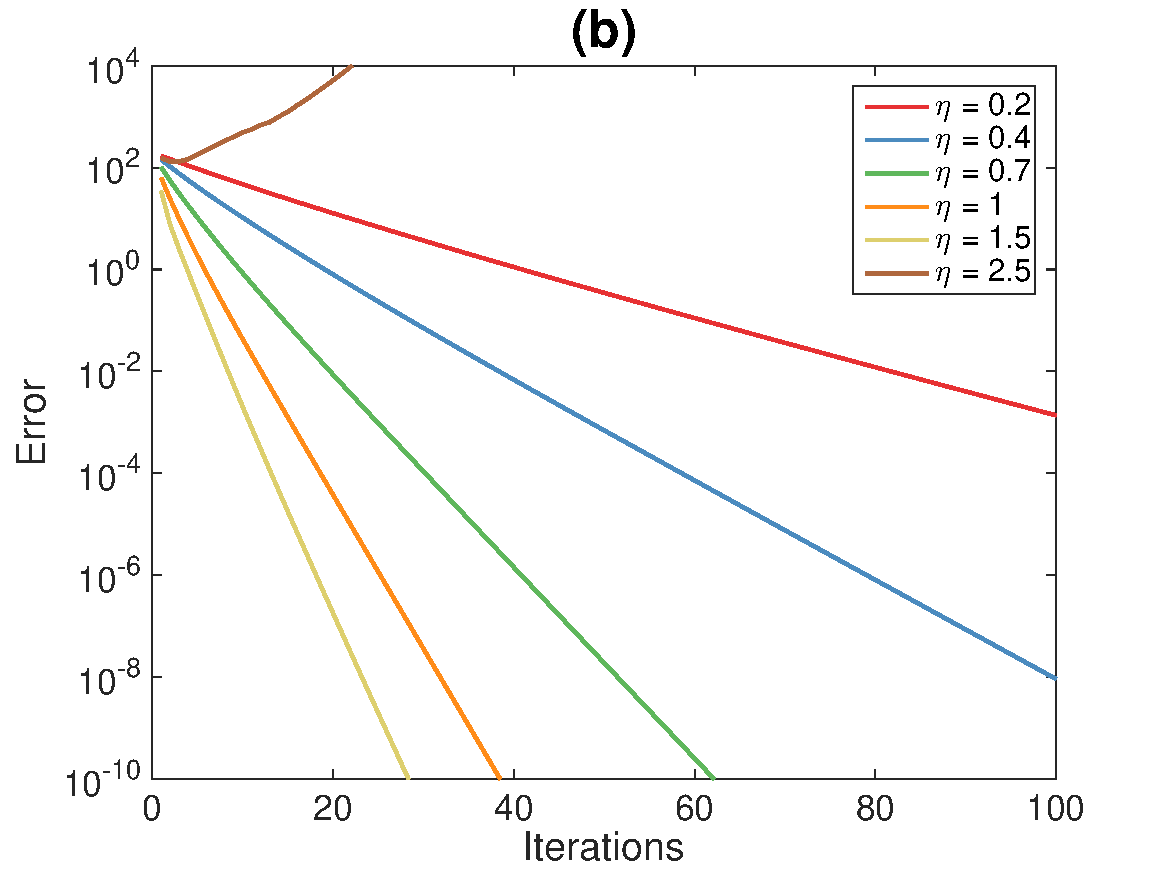
\includegraphics[width=0.49\textwidth]{figure/kappa13} 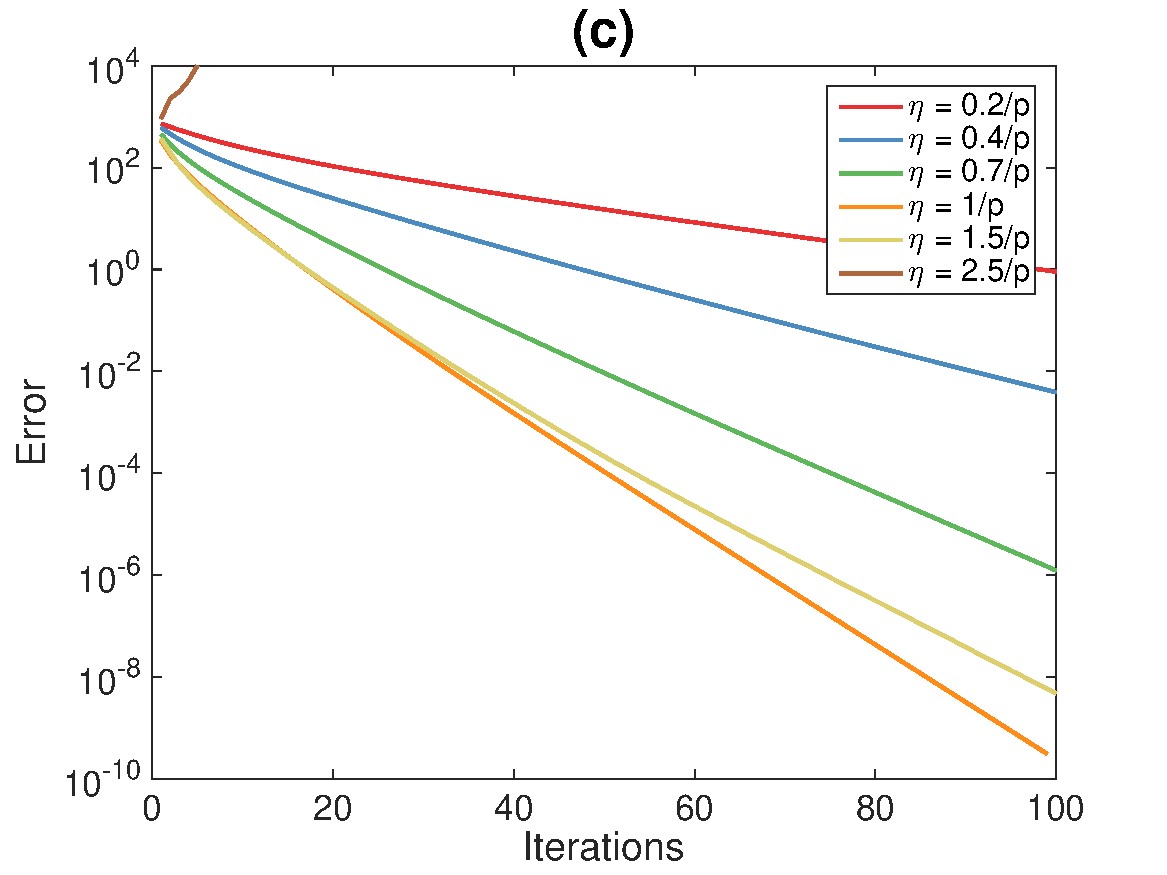
\includegraphics[width=0.49\textwidth]{figure/partial1b}
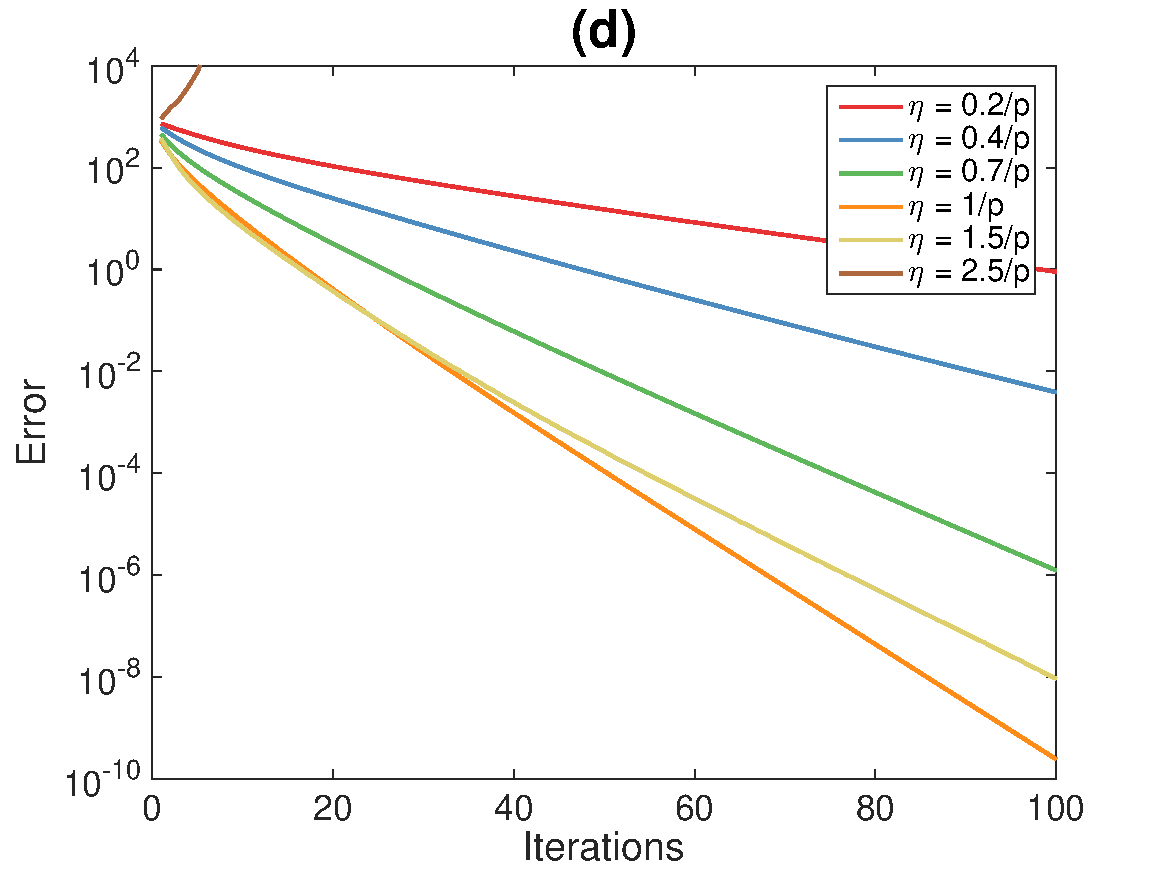
\includegraphics[width=0.49\textwidth]{figure/partial1c} \caption{The dependence of the estimation error on the number of iterations
for different step sizes $\eta$ (a) Algorithm~\ref{alg:gradient}
(Option 1); (b) Algorithm~\ref{alg:gradient} (Option 2); (c) Algorithm~\ref{alg:gradient2}
(Option 1); (d) Algorithm~\ref{alg:gradient2} (Option 2).}
\label{fig:options} 
\end{figure}

The second simulation concerns the choice of $\gamma$. We test $\gamma=c\gamma^{*}$
for a few choices of $c$ ($\gamma^{*}$ can be calculated from the
zero pattern of $\bS$). Figure \ref{fig:alpha} shows that if $\gamma$
is too small, for example, $0.5\gamma^{*}$, then the algorithm fail
to converge to the correct solution; and if $\gamma$ is too large,
then the convergence is slow. Following these observations, we use
$\gamma=1.5\gamma^{*}$ as the default choice of the following experiments,
which is also used in \cite{DBLP:conf/nips/YiPCC16}. 
\begin{figure}
\label{fig:alpha} \centering 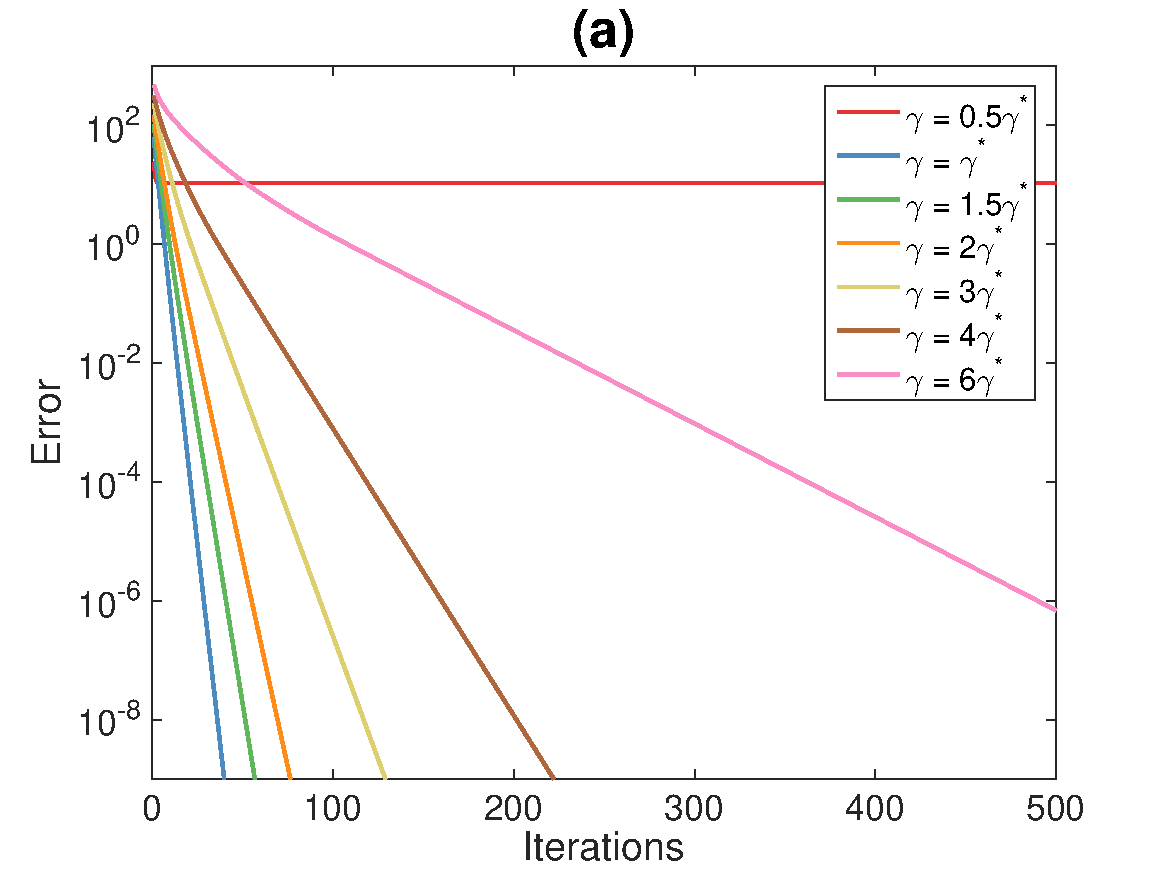
\includegraphics[width=0.49\textwidth]{figure/alpha1}
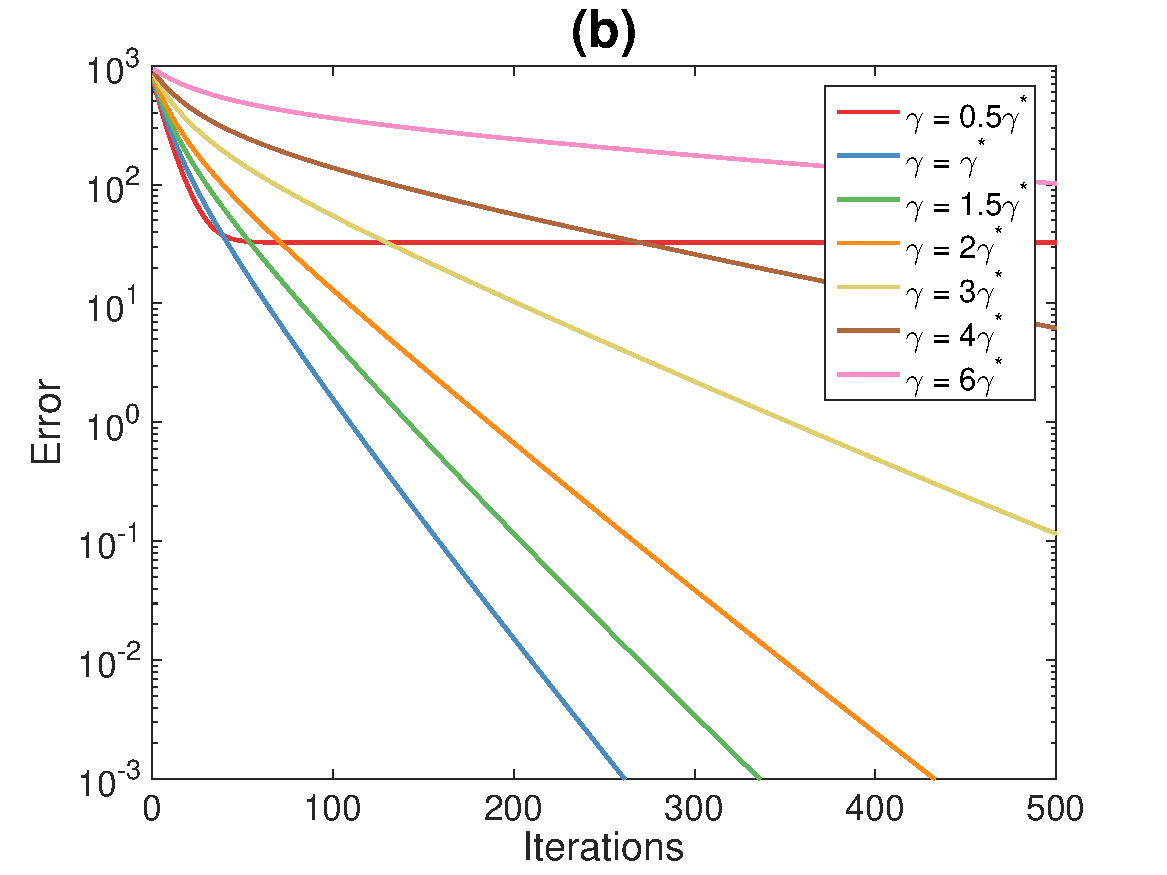
\includegraphics[width=0.49\textwidth]{figure/alpha2} \caption{The convergence of the algorithm depending on the choice of $\gamma$.
(a) fully observed setting; (b) partially observed setting.}
\end{figure}


\subsection{Performance of the proposed algorithm}

In this section, we analyze the convergence behavior as the parameters
(overall ratio of corrupted entries $q$, condition number $\kappa$,
rank $r$, subsampling ratio $p$) changes and visualized the result
in Figure~\ref{fig:performance}.

Figure~\ref{fig:performance}(a) shows the simulation for corruptions
level $q$, we use the setting in Section~\ref{sec:simu1}, but replace
the corruption level $q$ by $q=0.1,0.2,0.3,0.4$. Figure~\ref{fig:performance}
shows that the algorithm converges slower with more corruption, which
is expected since there is fewer information available. However, the
algorithm still converges even with an overall corruption level at
$0.4$.

Figure~\ref{fig:performance}(b) shows the simulation for rank $r$,
we use the setting in Section~\ref{sec:simu1}, but replace $r$
by $r=3,10,30,100,300$ respectively. Simulations show that the algorithm
works fine for rank $r=3,10,30,100$ and it converges slower for rank
$r=300$.

Figure~\ref{fig:performance}(c) shows the simulation for condition
number $\kappa$ of $\bL$, we use the setting in Section~\ref{sec:simu1},
but replace $\Sigma$ by $\Sigma=\diag(1,1,1/\kappa)$ and try various
values of $\kappa$. While the algorithm converges for $\kappa$ up
to $30$ in the simulation, for larger $\kappa$ the algorithm converges
slowly at the beginning, and then decreases quickly to zero. We suspect
that the initialization is not sufficiently good and it takes a while
for the algorithm to reach the ``local neighborhood of convergence''.
We also remark that $\bL$ with a very large condition number, e.g.
$\kappa=100$, is generally challenging for any nonconvex optimization
algorithm, as shown in Figure~\ref{fig:comparison}, Setting 4. It
is because that when $\kappa$ is large, the solution is close to
a matrix with rank less than $r$ -- a singular point on the manifold
of the matrices of rank $r$, which gives a geometry of manifold that
is not ``smooth'' enough. We observe that when $\kappa=100$, our
algorithm performs well if the rank $r$ is set to $2$ (instead of
the true value $3$)---in fact, when $\kappa=100$, the underlying
matrix is approximately of rank $2$ since the third singular value
is very small.

We test the algorithm with various matrix sizes using the setting
in Section~\ref{sec:simu1} and set $[n_{1},n_{2}]=[1000,1200],[5000,6000],[10000,12000]$.
Figure~\ref{fig:performance}(d) shows that Algorithm~\ref{alg:gradient}
converges quickly for all of the choices within a few iterations.

In the last simulation, we test Algorithm~\ref{alg:gradient2} under
the setting in Section~\ref{sec:simu1} with various choices of the
subsampling ratio $p$. Figure~\ref{fig:performance}(e) shows suggest
that the algorithm converges for $p$ as small as $0.1$, though the
convergence rate is slow for small $p$.

\begin{figure}
\centering 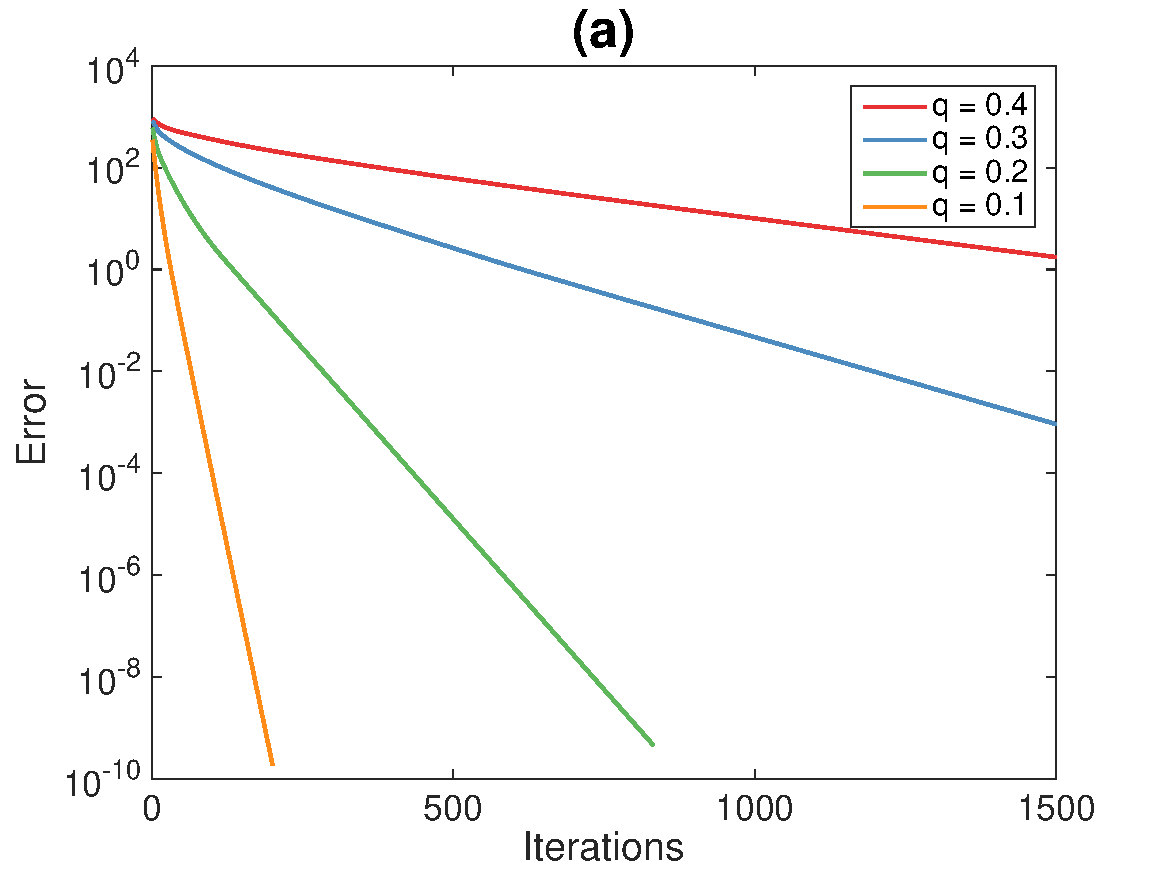
\includegraphics[width=0.49\textwidth]{figure/corruption}
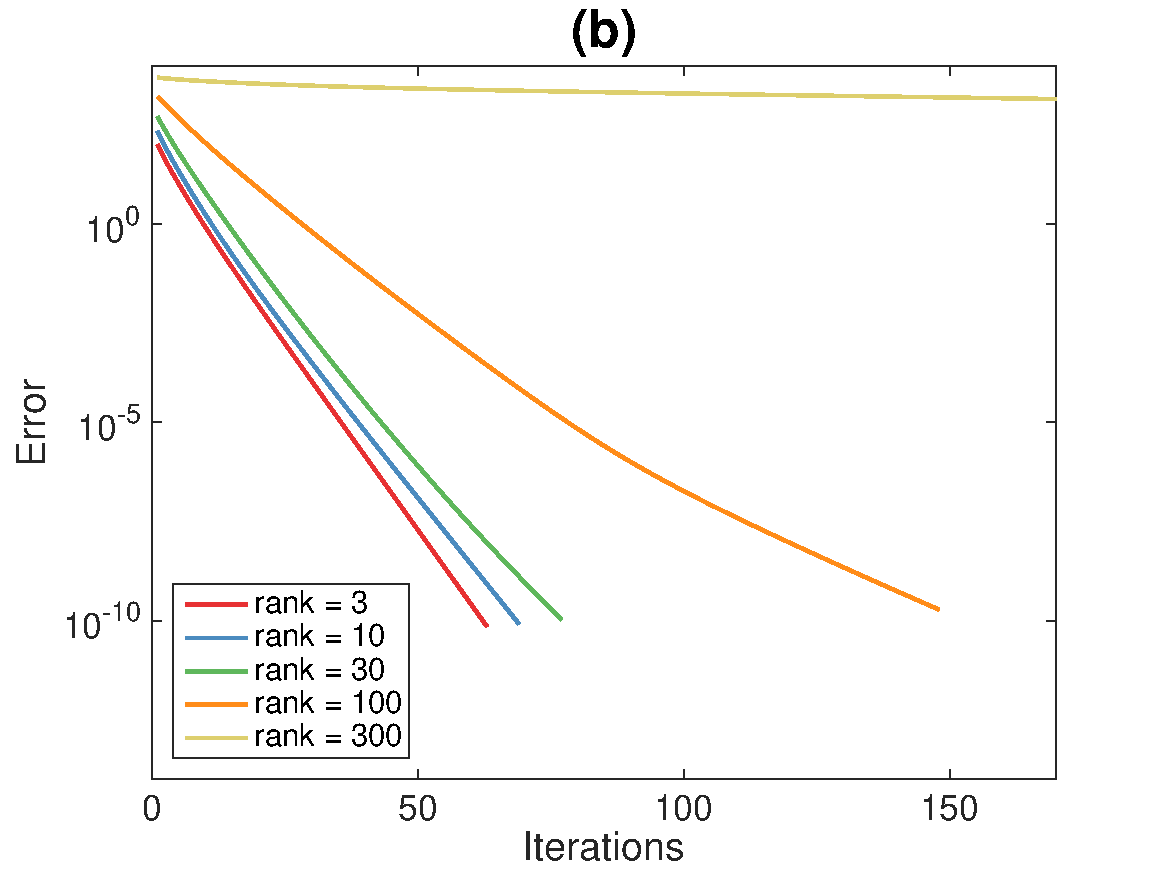
\includegraphics[width=0.49\textwidth]{figure/ranks} 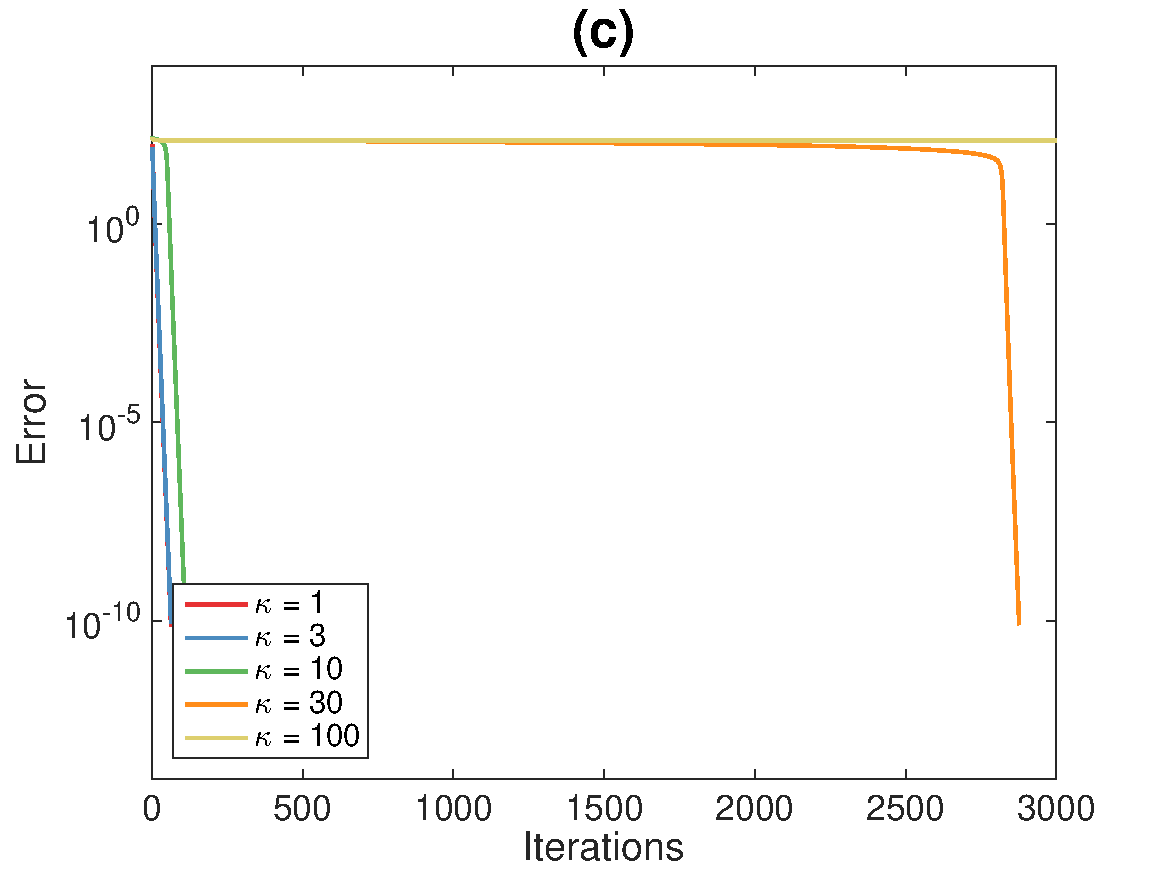
\includegraphics[width=0.49\textwidth]{figure/conditions}
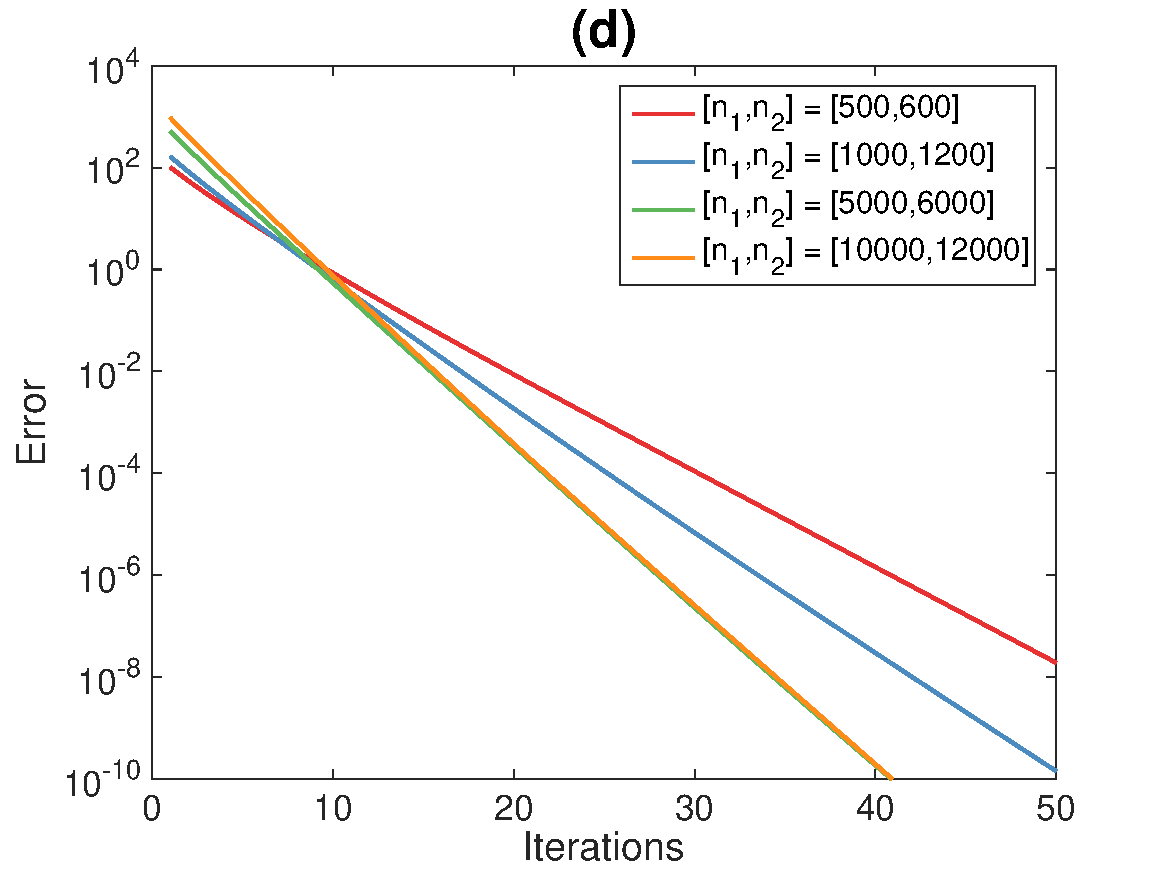
\includegraphics[width=0.49\textwidth]{figure/sizes} 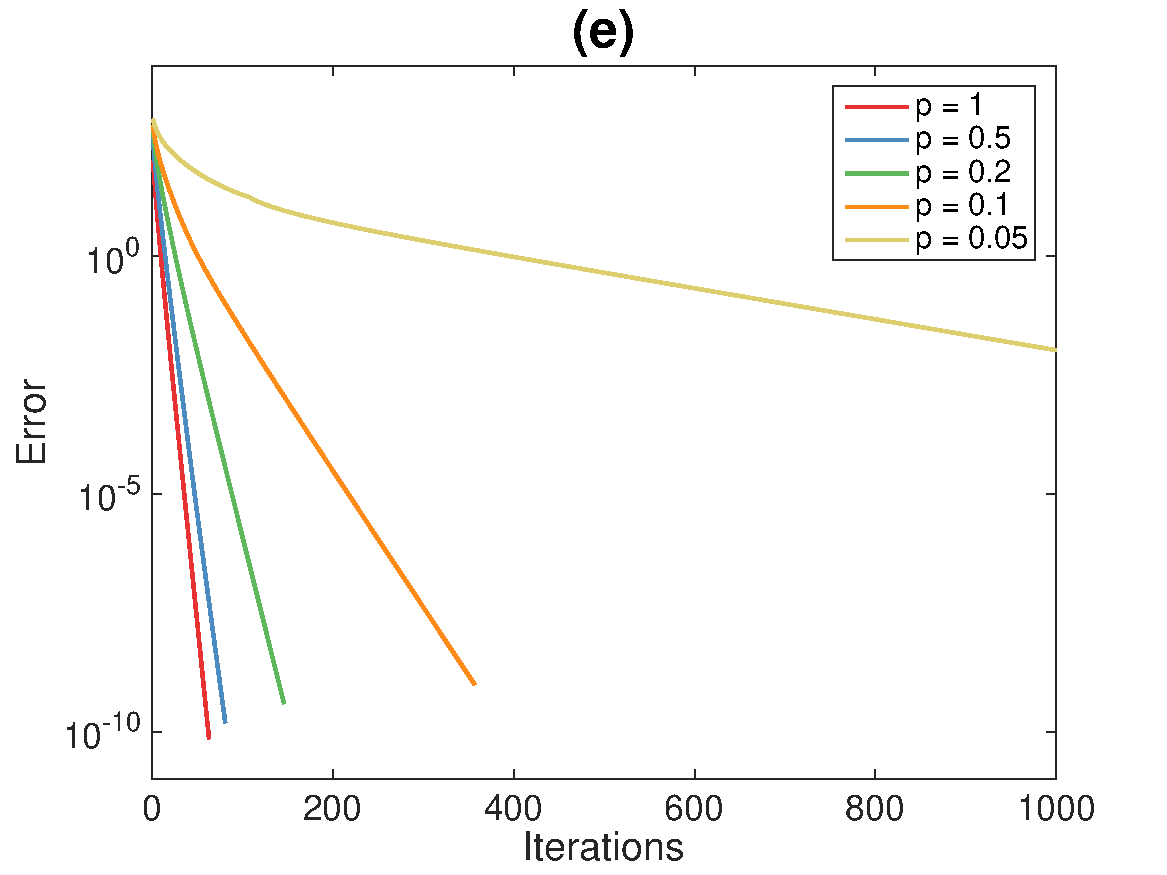
\includegraphics[width=0.49\textwidth]{figure/ratio}
\caption{Dependence of the estimation error on the number of iterations for
different (a) Overall ratios of corrupted entries $q$ (Algorithm
1); (b) Ranks $r$ (Algorithm 1); (c) Condition numbers $\kappa$
(Algorithm 1); (d) Matrix sizes $[n_{1},n_{2}]$ (Algorithm 1); (e)
Subsampling ratio $p$ (Algorithm 2).}
\label{fig:performance} 
\end{figure}


\subsection{Comparison with other robust PCA algorithms}

In this section, we compare our algorithm with the accelerated proximal
gradient method (APG) and the alternating direction method of multiplier
(ADMM) based on convex relaxation \eqref{eq:convex}; the robust matrix
completion algorithm (RMC) \cite{doi:10.1137/15M1025153} based on
manifold optimization problem 
\[
\argmin_{\rank(\bL)=r}\sum_{(i,j)\in\Phi}\|\bL_{ij}-\bY_{ij}\|+\lambda\sum_{(i,j)\not\in\Phi}\bL_{ij}^{2},
\]
as well as the alternating gradient descent method (AGD) in \cite{DBLP:conf/nips/YiPCC16}
that solves the same optimization as this work, but with an implementation
based on matrix factorization rather than manifold optimization. We
use the implementation of APG from \cite{Shen_anaccelerated} and
the implementation of ADMM from \url{https://github.com/dlaptev/RobustPCA}.
In these two algorithms, we use the choice of parameter $\lambda=1/\sqrt{\max(n_{1},n_{2})}$,
which is the default choice in the implementation \cite{Shen_anaccelerated}
and the theoretical analysis in \cite{robust_pca09}. For ADMM, the
augmented Lagrangian parameter is set by default as $10\lambda$.
For RMC and GD, we use their default setting of parameters. Since
the setting of Algorithm~\ref{alg:gradient2} does not apply to the
implementations of APG/ADMM, we compare them under the fully observed
setting. We compare them in the following four settings: 
\begin{itemize}
\item Setting 1: same setting as in Section~\ref{sec:simu1}. 
\item Setting 2 (large condition number): replace $\Sigma$ by $\diag(1,1,0.1)$
in Setting 1. 
\item Setting 3 (large matrix): replace $n_{1}$ and $n_{2}$ by $3000$
and $4000$ in Setting 1. 
\item Setting 4 (large condition number): replace $\Sigma$ by $\diag(1,1,0.01)$
in Setting 1. 
\end{itemize}
\begin{figure}
\centering 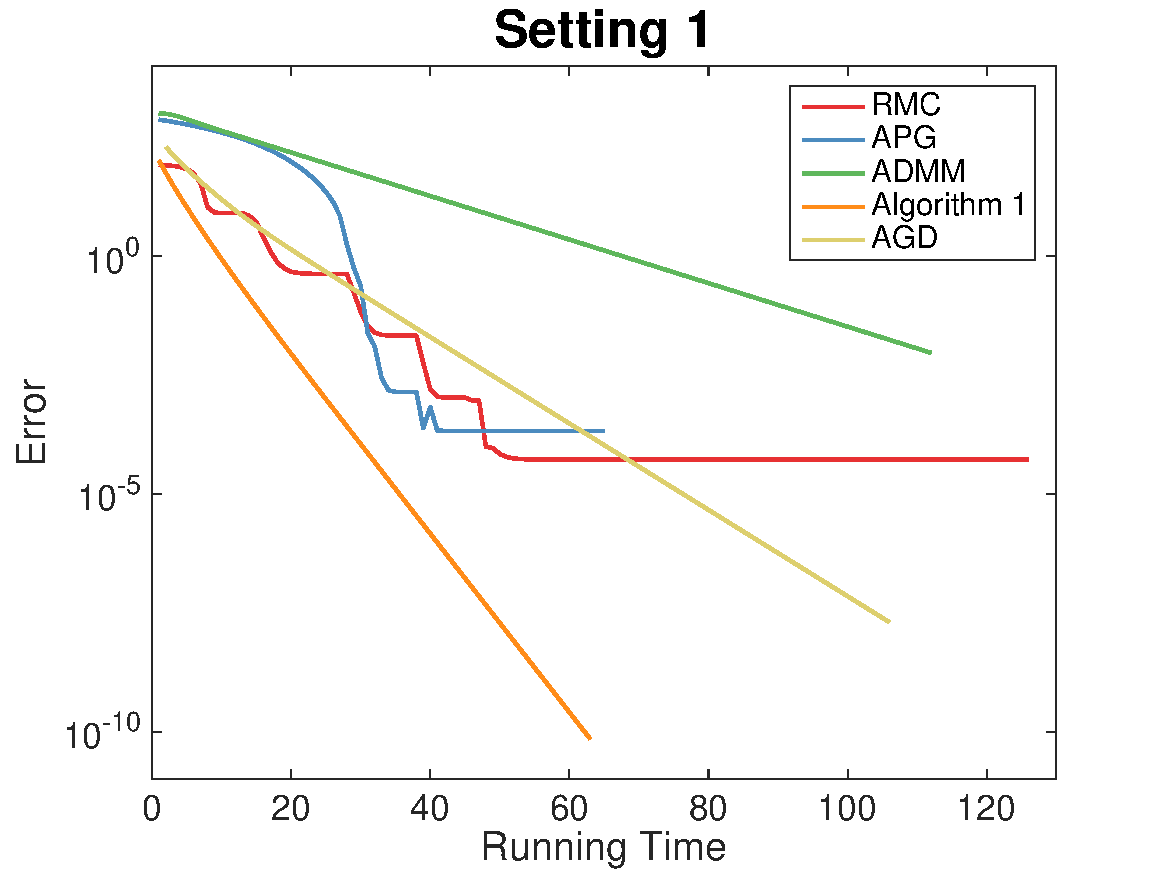
\includegraphics[width=0.49\textwidth]{figure/comparison1}
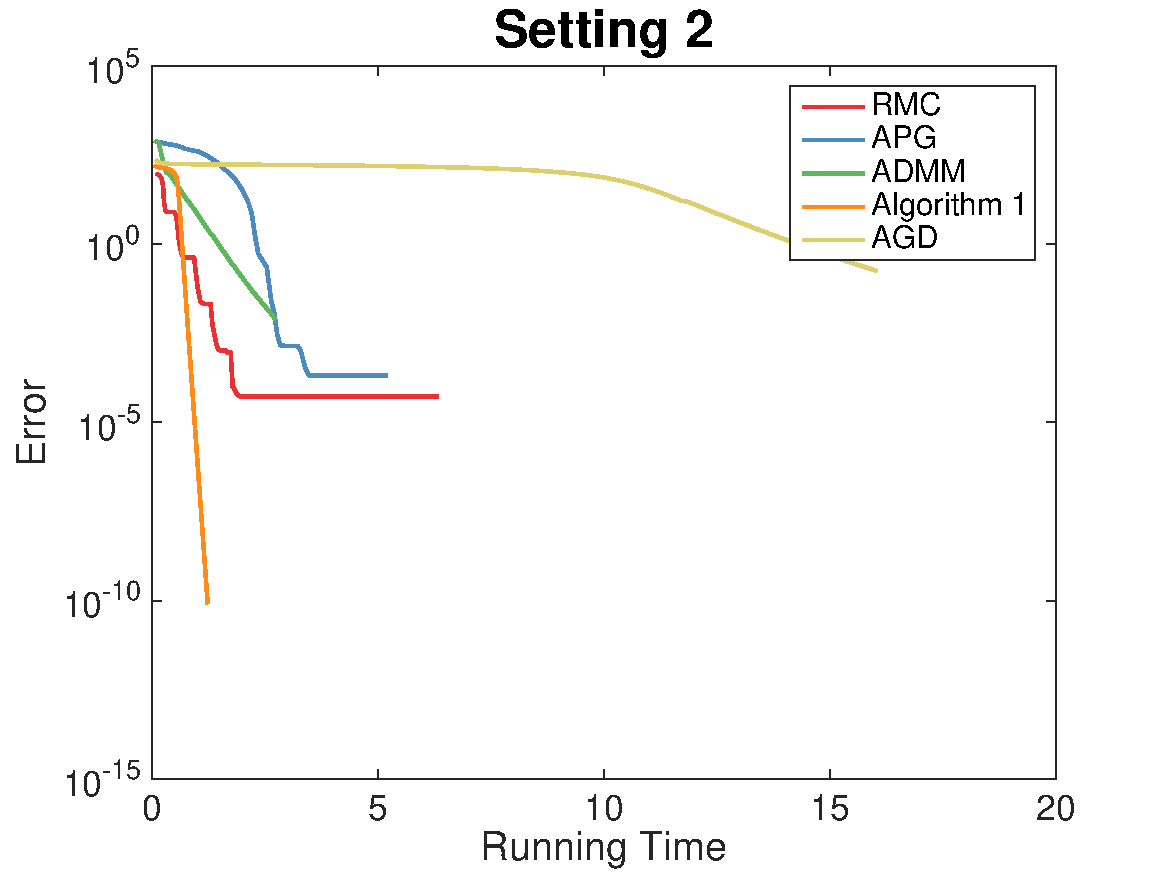
\includegraphics[width=0.49\textwidth]{figure/comparison2} 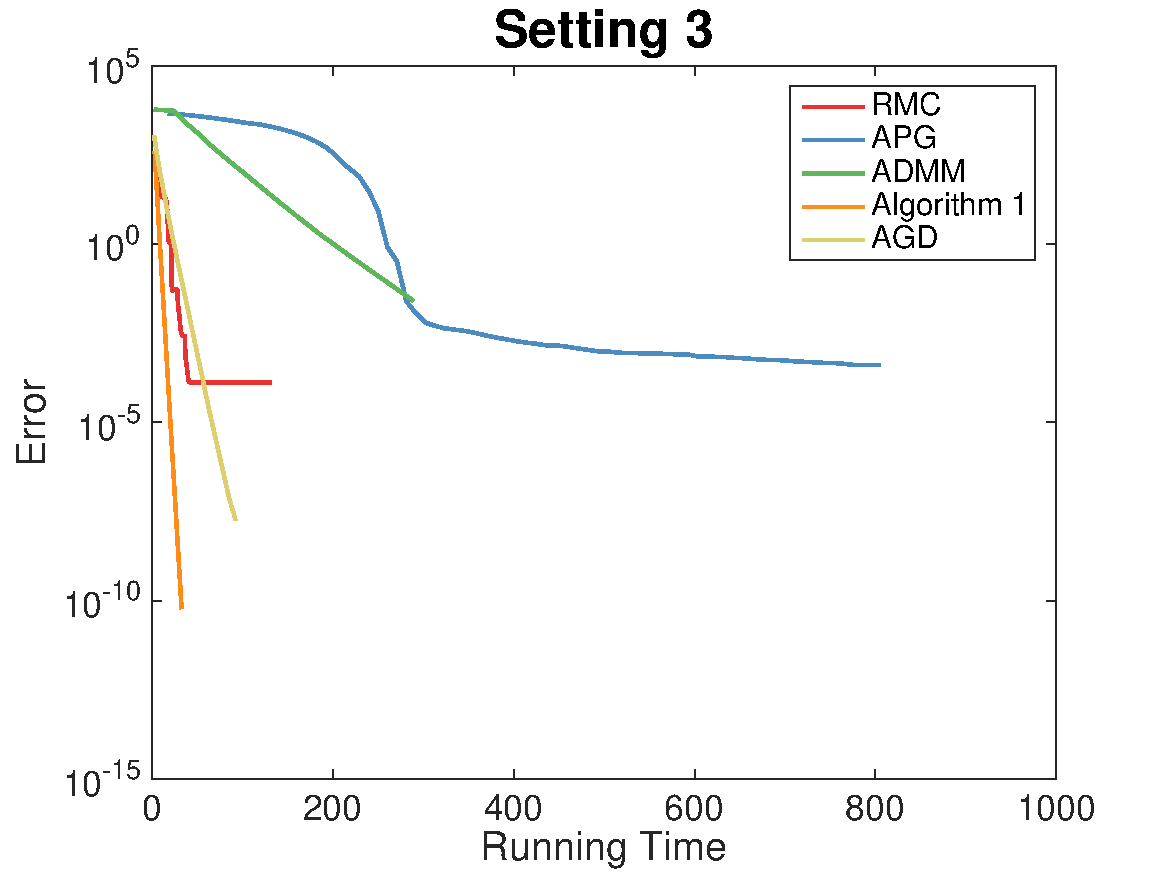
\includegraphics[width=0.49\textwidth]{figure/comparison3}
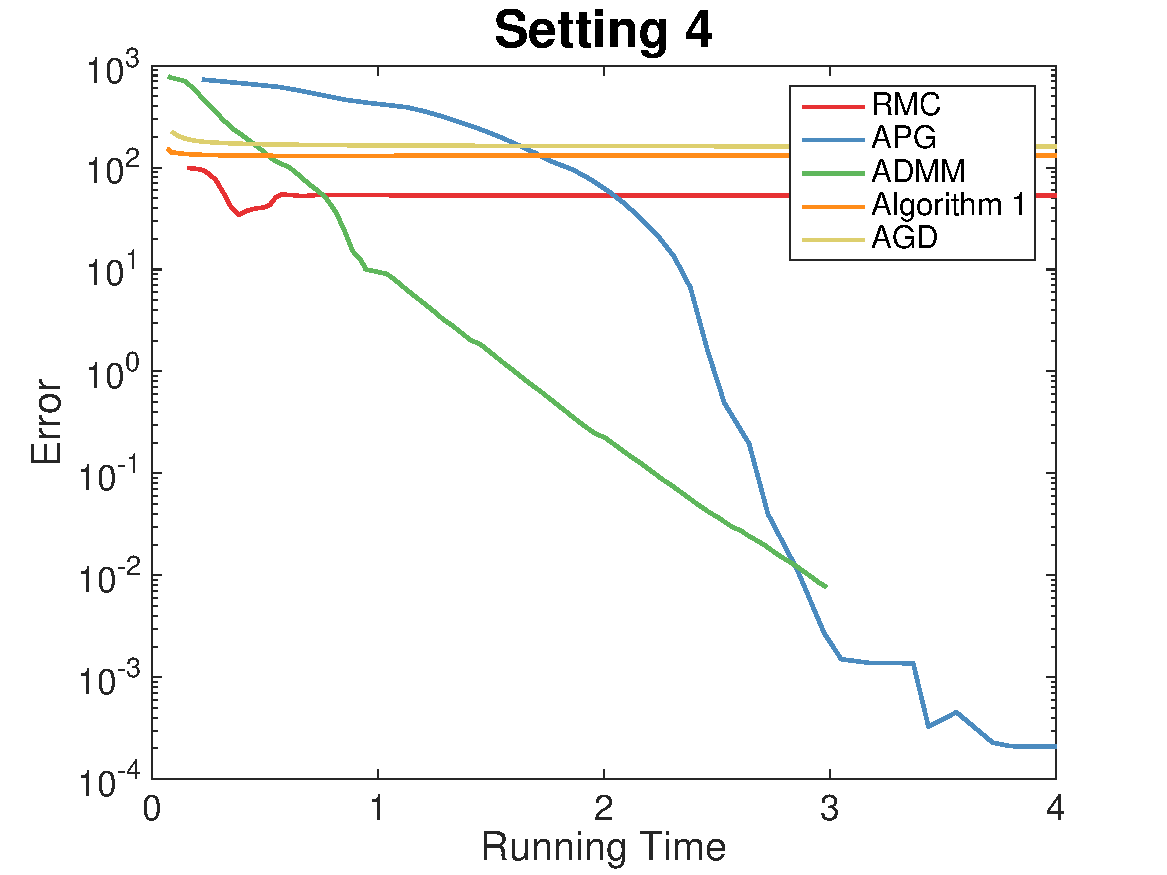
\includegraphics[width=0.49\textwidth]{figure/comparison4} \caption{The comparison of the performance of the algorithms under the fully
observed setting. The running time is measured in seconds.}
\label{fig:comparison} 
\end{figure}

Figure~\ref{fig:comparison} shows that under Setting 1, 2 and 3,
Algorithm~\ref{alg:gradient} converges faster than other algorithms.
In particular, the advantage over the AGD algorithm is very clear
under Setting 2, where the condition number is larger. This verifies
our theoretical analysis, where the convergence rate is faster than
the analysis in \cite{DBLP:conf/nips/YiPCC16} by a factor of $\sqrt{\kappa}$.
In Setting 3, the algorithms RMC, AGD and Algorithm~\ref{alg:gradient}
converge much faster than APG and ADMM, which verifies the computational
advantage of nonconvex algorithms when the matrix size is large. However,
in Setting 4, the convex algorithms converge to the correct solution
while the nonconvex algorithms converge to a local minimizer that
is different than the correct solution. This is due to the fact that
the nonconvex algorithms have more than one minimizer, and if it is
not initialized well then it could get trapped in local minimizers.
In practice, we observed that if the initialization is well chosen
and close to the true $\bL^{*}$, then Algorithm~\ref{alg:gradient}
converges quickly to the correct solution.

We also compare the performance of RMC, AGD and Algorithm~\ref{alg:gradient2}
under the partially observed setting. We use Setting 1 with $p=0.3$
and visualize the result in Figure~\ref{fig:partial}. The results
are similar to that of the fully observed setting: AGD and Algorithm~\ref{alg:gradient2}
are comparable and RMC converges faster at the beginning, but then
does not achieve higher accuracy, possibly due to their choice of
the regularization parameter. 
\begin{figure}
\centering 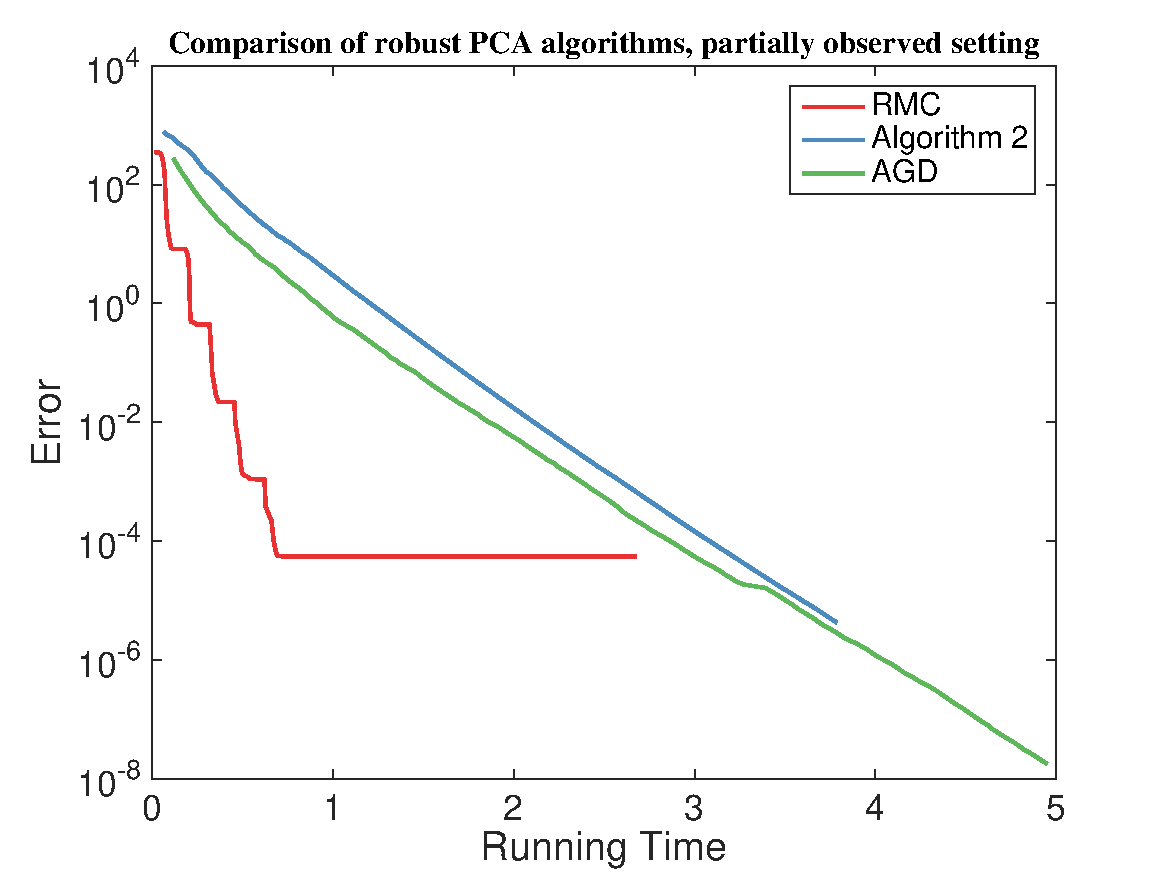
\includegraphics[width=0.65\textwidth]{figure/partial}
\caption{The comparison of the performances of the algorithms under the partially
observed setting. The running time is measured in seconds.}
\label{fig:partial} 
\end{figure}

We also test the proposed algorithms in a real data application for
video background subtraction. We adopt the public data set \texttt{Shoppingmall}
studied in \cite{DBLP:conf/nips/YiPCC16},\footnote{The data set is originally from \url{http://perception.i2r.a-star.edu.sg/bk_model/bk_index.html},
and is available at \url{https://sciences.ucf.edu/math/tengz/}.} A few frames are visualized in the first column of Figure~\ref{fig:DD3}.
There are 1000 frames in this video sequence, represented by a matrix
of size $81920\times1000$, where each column corresponds to a frame
of the video and each row corresponds to a pixel of the video. We
apply our algorithms with $r=3$ and $\gamma^{*}=0.1$, $p=0.5$ for
the partially observed case, the step size $\eta=0.7$. We stop the
algorithm after 100 iterations. Figure~\ref{fig:DD3} shows that
our algorithms obtain desirable low-rank approximations within $100$
iterations.

In Figure~\ref{fig:DD4}, we compare our algorithms with APG in terms
of  the convergence of the objective function value. In this figure,
the relative error is defined as $\|F(\bL-\bY)\|_{F}/\|\bY\|_{F}$,
a scaled objective value. A smaller relative error implies a better
low-rank approximation. Figure~\ref{fig:DD4} shows out that our
algorithms can obtain smaller objective values within 100 iterations
under both fully observed and partially observed cases.

\begin{figure}
\centering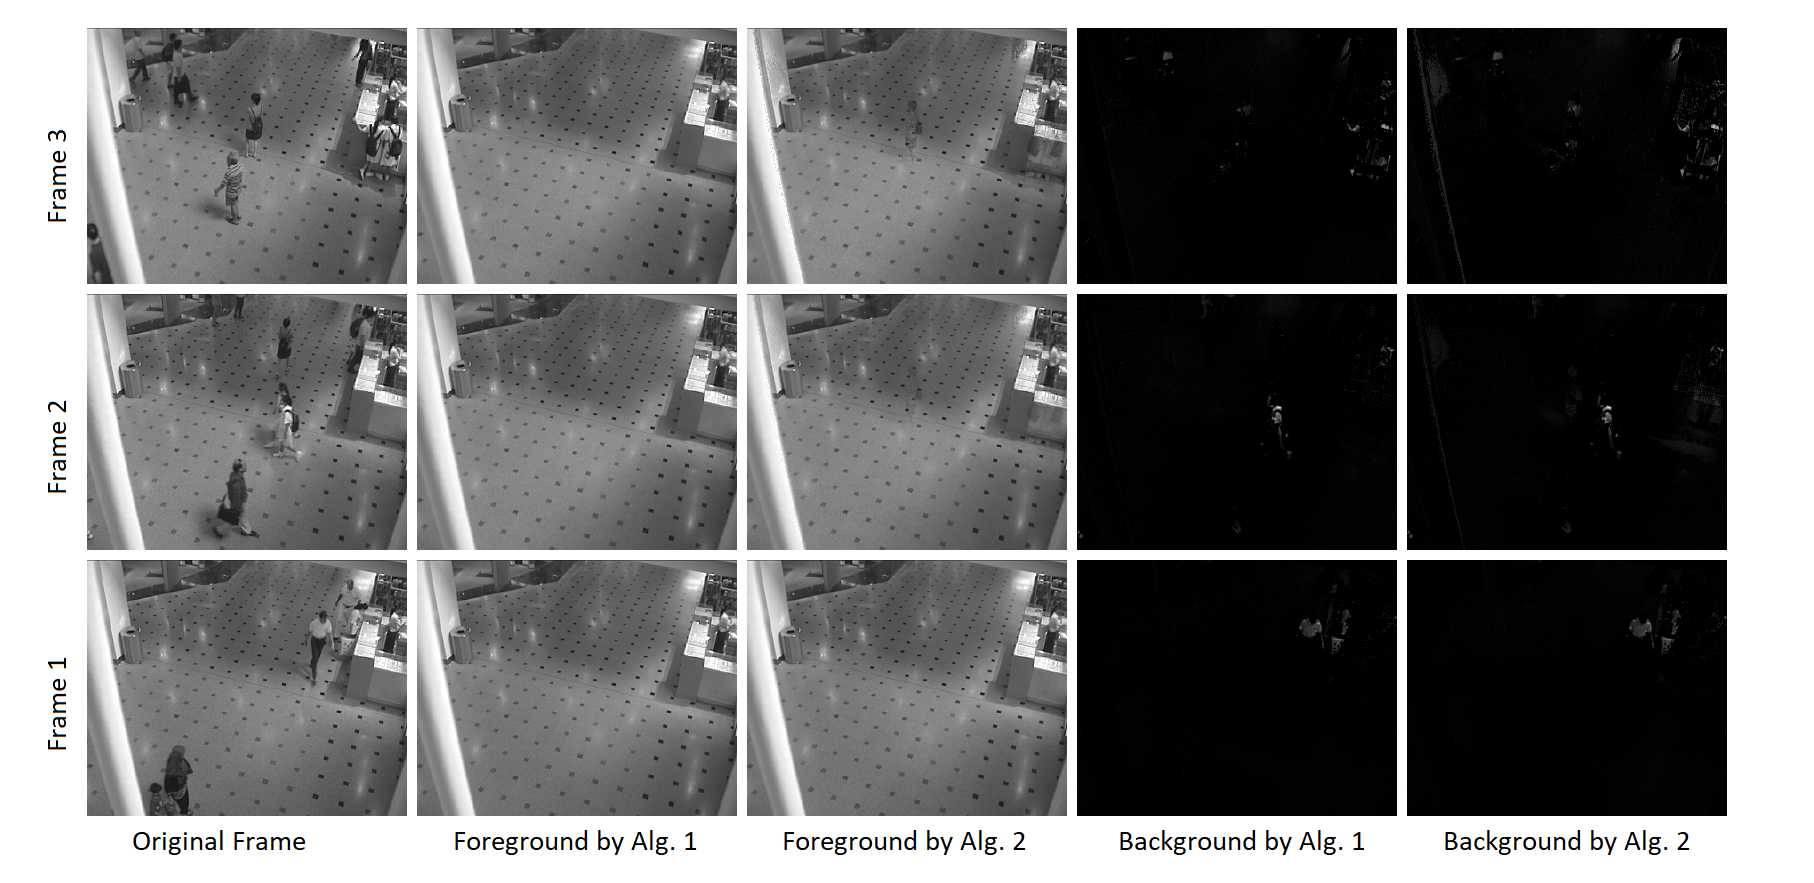
\includegraphics[width=1\textwidth]{figure/simu3} \caption{The performance of Algorithms~\ref{alg:gradient} and~\ref{alg:gradient2}
in video background subtraction, with three rows representing three
frames in the video sequence. For Algorithm~\ref{alg:gradient2},
a subsampling ratio of $p=0.5$ is used.}
\label{fig:DD3} 
\end{figure}

\begin{figure}
\centering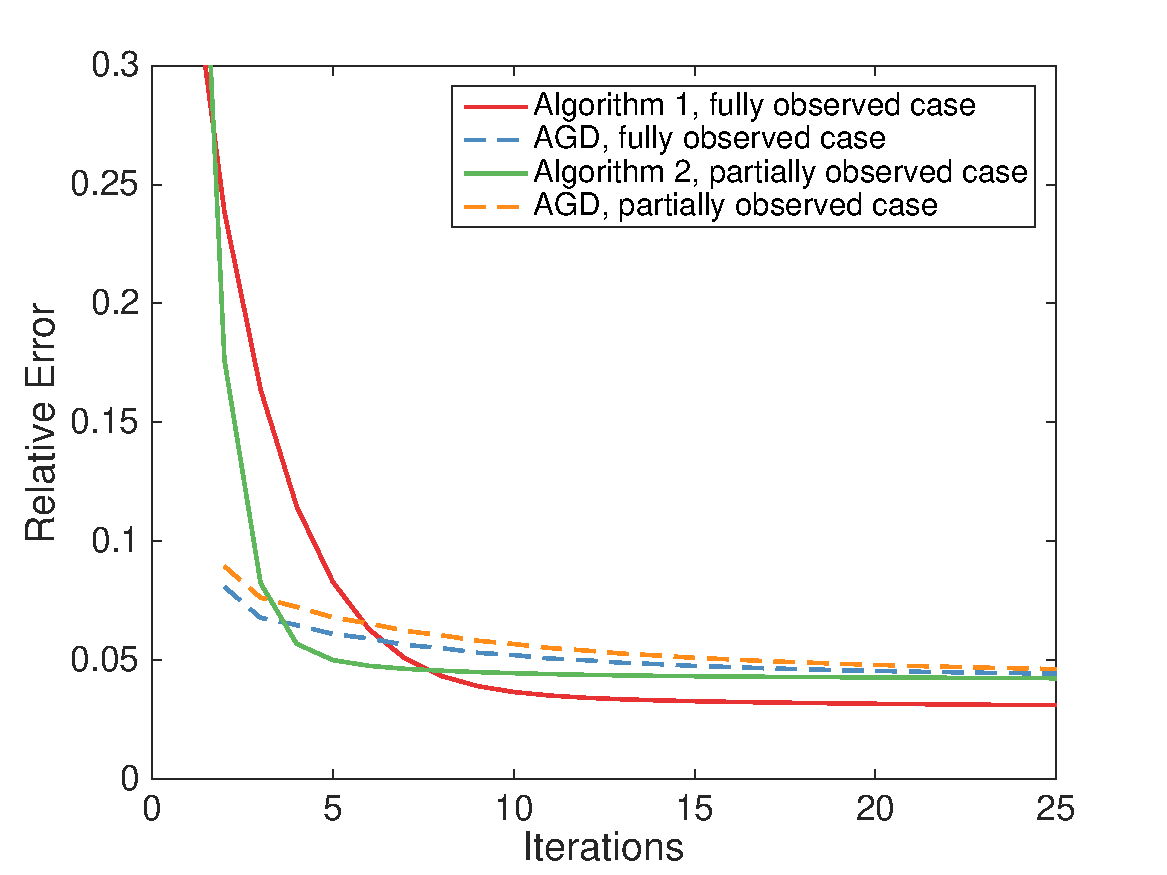
\includegraphics[width=0.65\textwidth]{figure/shoppingmall_obj}%\includegraphics[width=0.49\textwidth]{figure/our_full.png}
%\centering\includegraphics[width=0.49\textwidth]{figure/their_partial.png}\includegraphics[width=0.49\textwidth]{figure/our_partial.png}
\caption{The relative error of Algorithms~\ref{alg:gradient}, \ref{alg:gradient2},
and AGD with respect to the iterations, for both fully observed case
and partially observed case in the experiment of background subtraction.}
\label{fig:DD4} 
\end{figure}


\section{Conclusion}

\label{sec:discussion} This paper proposes two robust PCA algorithms
(one for fully observed case and one for partially observed case)
based on the gradient descent algorithm on the manifold of low-rank
matrices. Theoretically, compared with the gradient descent algorithm
with matrix factorization, our approach has a faster convergence rate,
better tolerance of the initialization accuracy and corruption level.
The approach removes or reduces the dependence of the algorithms on
the condition number of the underlying low-rank matrix. Numerically,
the proposed algorithms performance is less sensitive to the choice
of step sizes. We also find that under the partially observed setting,
the performance of the proposed algorithm is not significantly affected
by the presence of the additional dependence on the observation probability.
Considering the popularity of the methods based on matrix factorization,
it is an interesting future direction to apply manifold optimization
to other low-rank matrix estimation problems. 

\section*{Acknowledgements}

The authors thank the editor, an associate editor and referee for
their helpful comments and suggestions. The authors also thank David
Fleischer for providing helps on the coding. Yang's research is partially
supported by NSERC RGPIN-2016-05174. Zhang's research is partially supported by National Science Foundation (NSF) grant CNS-1739736.

\newpage
\section*{Appendix for ``Robust PCA by Manifold Optimization\textquotedbl}

\subsection*{A. Technical Derivations in Section~\ref{sec:review_algo}}

\paragraph*{Verification of \eqref{eq:projection}.}

Formula \eqref{eq:projection} can be verified as follows. Let $\langle\cdot\rangle_{F}$
be the Frobenius inner product of two matrices, then 
\begin{align*}
 & \langle\bD-P_{T_{\bX}\calM}(\bD),\bA\bV\bV^{T}\rangle_{F}=\langle(\bI-\bU\bU^{T})\bD(\bI-\bV\bV^{T}),\bA\bV\bV^{T}\rangle_{F}\\
= & \langle(\bI-\bU\bU^{T})\bD(\bI-\bV\bV^{T})\bV\bV^{T},\bA\rangle_{F}=\langle\mathbf{0},\bA\rangle_{F}=0
\end{align*}
and similarly $\langle\bD-P_{T_{\bX}\calM}(\bD),\bU\bU^{T}\bB\rangle_{F}=0$.
As a result, $\langle\bD-P_{T_{\bX}\calM}(\bD),\bA\bV\bV^{T}+\bU\bU^{T}\bB\rangle_{F}=0$
for all $\bA\in\reals^{n_{1}\times n_{1}}$ and $\bB\in\reals^{n_{2}\times n_{2}}$,
which verifies formula \eqref{eq:projection} by showing that $\bD-P_{T_{\bX}\calM}(\bD)$
is orthogonal to $T_{\bX}\calM$.

\paragraph*{Verification of \eqref{eq:ortho_retraction}.}

It is clear that $R_{\bX}^{(2)}(\bd)$ defined in \eqref{eq:ortho_retraction}
has rank $r$; and to show that $\langle R_{\bX}^{(2)}(\bd)-(\bX+\bd),\bZ\rangle_{F}=0\,\,\text{for all \ensuremath{\bZ\in T_{\bX}\calM}}$,
we first write this property as $[R_{\bX}^{(2)}(\bd)-(\bX+\bd)]\perp T_{\bX}\calM$
for simplicity, and since $T_{\bX}\calM=\{\bA\bV\bV^{T}+\bU\bU^{T}\bB:\text{for}\,\,\bA\in\reals^{n_{1}\times n_{1}},\bB\in\reals^{n_{2}\times n_{2}}\}$,
we just need to show that $\langle R_{\bX}^{(2)}(\bd)-(\bX+\bd),\bA\bV\bV^{T}+\bU\bU^{T}\bB\rangle_{F}=0$
for all $\bA\in\reals^{n_{1}\times n_{1}}$ and $\bB\in\reals^{n_{2}\times n_{2}}$.
This is easy to verify, because we have $R_{\bX}^{(2)}(\bd)\bV=(\bX+\bd)\bV$,
\begin{equation}
\langle R_{\bX}^{(2)}(\bd)-(\bX+\bd),\bA\bV\bV^{T}\rangle_{F}=\langle(R_{\bX}^{(2)}(\bd)\bV-(\bX+\bd)\bV)\bV^{T},\bA\rangle_{F}=\langle\mathbf{0},\bA\rangle_{F}=0,
\end{equation}
Similarly, we can easily verify that $\bU^{T}R_{\bX}^{(2)}(\bd)=\bU^{T}(\bX+\bd)$,
we have $\langle R_{\bX}^{(2)}(\bd)-(\bX+\bd),\bU\bU^{T}\bB\rangle_{F}=0$,
and therefore $[R_{\bX}^{(2)}(\bd)-(\bX+\bd)]\perp T_{\bX}\calM$.
As a result, there exists a unique $R_{\bX}^{(2)}$ such that $\rank(R_{\bX}^{(2)})=r$
and $[R_{\bX}^{(2)}(\bd)-(\bX+\bd)]\perp T_{\bX}\calM$.

\paragraph*{Verification of \eqref{eq:derivative}.}

We first define the operator $S:\reals^{n_{1}\times n_{2}}\rightarrow\reals^{n_{1}\times n_{2}}$
such that $F(\bA)=\bS(\bA)\circ\bA$ ($\circ$ represents the elementwise
product), i.e., 
\[
\bS(\bA)=\begin{cases}
0,\,\,\,\,\text{if \ensuremath{|\bA_{ij}|>|\bA_{i,\cdot}|^{[\gamma]}} and \ensuremath{|\bA_{ij}|>|\bA_{\cdot,j}|^{[\gamma]}},}\\
1,\,\,\,\,\text{otherwise.}
\end{cases}
\]

Then if the absolute values of all entries of $\bA$ are different,
the sparsity pattern does not change under a small perturbation, i.e.,
$\bS(\bA)=\bS(\bA+\bDelta).$ Then by definition of $f(\cdot)$, 
\begin{align*}
 & f(\bL+\bDelta)-f(\bL)=\frac{1}{2}\|\bS(\bL-\bY+\bDelta)\circ(\bL-\bY+\bDelta)\|_{F}^{2}-\frac{1}{2}\|\bS(\bL-\bY)\circ(\bL-\bY)\|_{F}^{2}\\
= & \frac{1}{2}\|\bS(\bL-\bY)\circ(\bL-\bY+\bDelta)\|_{F}^{2}-\frac{1}{2}\|\bS(\bL-\bY)\circ(\bL-\bY)\|_{F}^{2}\\
= & \langle\bS(\bL-\bY)\circ(\bL-\bY),\bDelta\rangle_{F}+O(\|\bDelta\|_{F}^{2}),
\end{align*}
where $\circ$ represents the Hadamard product, i.e., the elementwise
product between matrices.

\paragraph*{Verification of \eqref{eq:ortho_retraction1}.}

It is sufficient to prove the case where $\bU^{(k)}$ and $\bV^{(k)}$
are given by the SVD decomposition $\bL^{(k)}=\bU^{(k)}\bSigma^{(k)}\bV^{(k)T}$.
Denote $\bD=\grad f(\bL^{(k)})=F(\bL^{(k)}-\bY)$. Set $\bX=\bL^{(k)}$
and $\bd=-\eta P_{T_{\bL^{(k)}}\calM}(\bD)$ in \eqref{eq:ortho_retraction},
we have 
\begin{eqnarray}
\bL^{(k+1)} & \coloneqq & (\bL^{(k)}-\eta P_{T_{\bL^{(k)}}\calM}(\bD))\bV^{(k)}[\bU^{(k)T}(\bL^{(k)}-\eta P_{T_{\bL^{(k)}}\calM}(\bD))\bV^{(k)}]^{-1}\label{eq:inter}\\
 &  & \bU^{(k)T}(\bL^{(k)}-\eta P_{T_{\bL^{(k)}}\calM}(\bD))\nonumber 
\end{eqnarray}
On the other hand, from \eqref{eq:projection} we have the projection
\[
P_{T_{\bL^{(k)}}\calM}(\bD)=\bU^{(k)}\bU^{(k)T}\bD+\bD\bV^{(k)}\bV^{(k)T}-\bU^{(k)}\bU^{(k)T}\bD\bV^{(k)}\bV^{(k)T}.
\]
As a result 
\begin{align}
 & P_{T_{\bL^{(k)}}\calM}(\bD)\bV^{(k)}=[\bU^{(k)}\bU^{(k)T}\bD+\bD\bV^{(k)}\bV^{(k)T}-\bU^{(k)}\bU^{(k)T}\bD\bV^{(k)}\bV^{(k)T}]\bV^{(k)}\nonumber \\
 & =\bU^{(k)}\bU^{(k)T}\bD\bV^{(k)}+\bD\bV^{(k)}\bV^{(k)T}\bV^{(k)}-\bU^{(k)}\bU^{(k)T}\bD\bV^{(k)}\bV^{(k)T}{\bV^{(k)}}=\bD\bV^{(k)}\label{eq:dv}
\end{align}
and similarly, 
\begin{equation}
\bU^{(k)T}P_{T_{\bL^{(k)}}\calM}(\bD)=\bU^{(k)T}\bD.\label{eq:projection2}
\end{equation}
Combining \eqref{eq:dv}, \eqref{eq:projection2} with \eqref{eq:inter},
the update formula \eqref{eq:ortho_retraction1} is verified.

\subsection*{B. Proof of Theorem~\ref{thm:main}}

In this proof, we will investigate $\|\bL^{+}-\bL^{*}\|_{F}$, where
\[
\bL^{+}=R_{\bL}(-\eta P_{T_{\bL}}F(\bL-\bY)).
\]
It is sufficient to prove that when $\|\bL-\bL^{*}\|\leq a\sigma_{r}(\bL^{*})$
with the value $a$ satisfying the conditions in Theorem~\ref{thm:main},
then 
\begin{equation}
\|\bL^{+}-\bL^{*}\|_{F}\leq\Big(1-\frac{1-2C_{1}}{8}\eta\Big)\|\bL-\bL^{*}\|_{F}.\label{eq:goal1}
\end{equation}
To prove \eqref{eq:goal1}, we first introduce three auxiliary lemmas. 
\begin{lemma}
\label{lemma:bD} 
\begin{description}
\item [{(a)}] Let $\bD=\bL-\bL^{*}-F(\bL-\bY)=\bL-\bL^{*}-F(\bL-\bL^{*}-\bS^{*})$,
then 
\begin{equation}
\|\bD\|_{F}^{2}\leq C_{1}^{2}\|\bL-\bL^{*}\|_{F}^{2}.\label{eq:second_bound}
\end{equation}
\item [{(b)}] For the noisy setting where $\bY=\bL^{*}+\bS^{*}+\bN^{*}$,
and $\bD'=\bL-\bL^{*}-\bN^{*}-F(\bL-\bY)$, we have 
\begin{equation}
\|\bD'\|_{F}^{2}\leq2C_{1}^{2}\|\bL-\bL^{*}\|_{F}^{2}+2(\gamma+5\gamma^{*})N_{1},\label{eq:second_bound_noisy}
\end{equation}
where $N_{1}=n_{2}\sum_{i=1}^{n_{1}}|\bN_{i,\cdot}^{*}|^{\max}+n_{1}\sum_{j=1}^{n_{2}}|\bN_{\cdot,j}^{*}|^{\max}$. 
\end{description}
\end{lemma}
%
\begin{lemma}
\label{lemma:approximation} If $\|\bL-\bL^{*}\|_{F}\leq a\sigma_{r}(\bL^{*})$
and $a\leq1$, then 
\begin{align}
\|(\bL-\bL^{*})-\bP_{T_{\bL}}(\bL-\bL^{*})\|_{F}\leq & \frac{a}{2(1-a)}\|\bL-\bL^{*}\|_{F},\label{eq:control1}\\
\|(\bL-\bL^{*})-\bP_{T_{\bL^{*}}}(\bL-\bL^{*})\|_{F}\leq & \frac{a}{2}\|\bL-\bL^{*}\|_{F}.\label{eq:control2}
\end{align}
\end{lemma}
%
\begin{lemma}
\label{lemma:retraction} For $\bX\in T_{\bL}\calM$, then 
\[
\|R_{\bL}^{(i)}(\bX)-(\bL+\bX)\|_{F}\leq\frac{\|\bX\|_{F}^{2}}{2(\sigma_{r}(\bL)-\|\bX\|)},\,\,\text{for either \ensuremath{i=1} or \ensuremath{2}.}
\]
\end{lemma}
To prove \eqref{eq:goal1}, first we note that 
\begin{align}
 & \|\bL-\bL^{*}\|_{F}^{2}-\|\bL-\eta P_{T_{\bL}}F(\bL-\bY)-\bL^{*}\|_{F}^{2}\nonumber \\
= & \|\bL-\bL^{*}\|_{F}^{2}-\|\bL-\bL^{*}\|_{F}^{2}+2\eta\langle\bL-\bL^{*},P_{T_{\bL}}F(\bL-\bY)\rangle_{F}-\|\eta P_{T_{\bL}}F(\bL-\bY)\|_{F}^{2}\nonumber \\
= & 2\eta\langle\bL-\bL^{*},P_{T_{\bL}}F(\bL-\bY)\rangle_{F}-\|\eta P_{T_{\bL}}F(\bL-\bY)\|_{F}^{2}\nonumber \\
= & 2\eta\langle\bL-\bL^{*},P_{T_{\bL}}(\bL-\bL^{*})-P_{T_{\bL}}(\bL-\bL^{*}-F(\bL-\bY))\rangle_{F}-\eta^{2}\|P_{T_{\bL}}F(\bL-\bY)\|_{F}^{2}\nonumber \\
= & 2\eta\langle P_{T_{\bL}}(\bL-\bL^{*}),P_{T_{\bL}}(\bL-\bL^{*})-P_{T_{\bL}}\bD\rangle_{F}-\eta^{2}\|P_{T_{\bL}}F(\bL-\bY)\|_{F}^{2}\nonumber \\
\geq & 2\eta(\|P_{T_{\bL}}(\bL-\bL^{*})\|_{F}^{2}-\|\bD\|_{F}\|P_{T_{\bL}}(\bL-\bL^{*})\|_{F})-\eta^{2}(\|\bL-\bL^{*}\|_{F}+\|\bD\|_{F})^{2}.\label{eq:condition1}
\end{align}
The fourth line is obtained by $P_{T_{\bL}}(\bL-\bL^{*}-F(\bL-\bY))=\bL-\bL^{*}-P_{T_{\bL}}F(\bL-\bY)\rangle_{F}$.
The fifth line is because $\bL-\bL^{*}=P_{T_{\bL}}(\bL-\bL^{*})+P_{T_{\bL}}^{\perp}(\bL-\bL^{*})$.
The last line uses Cauchy-Schwarz inequality $\langle P_{T_{\bL}}(\bL-\bL^{*}),P_{T_{\bL}}\bD\rangle_{F}\leq\|\bD\|_{F}\|P_{T_{\bL}}(\bL-\bL^{*})\|_{F}$
and triangular inequality $\|P_{T_{\bL}}F(\bL-\bY)\|_{F}\leq\|\bL-\bL^{*}\|_{F}+\|P_{T_{\bL}}(\bD)\|_{F}\leq\|\bL-\bL^{*}\|_{F}+\|\bD\|_{F}$.
Lemma~\ref{lemma:approximation} and the assumptions $\|\bL-\bL^{*}\|_{F}\leq a\sigma_{r}(\bL^{*})$
and $\sqrt{1-(\frac{a}{2(1-a)})^{2}}>\frac{1}{2}$ imply 
\begin{equation}
\|P_{T_{\bL}}(\bL-\bL^{*})\|_{F}\geq\frac{1}{2}\|\bL-\bL^{*}\|_{F}.\label{eq:condition1.5}
\end{equation}
Combining it with the estimation of $\|\bD\|_{F}$ in Lemma~\ref{lemma:bD},
we have 
\begin{align}
\|\bL-\bL^{*}\|_{F}^{2}-\|\bL-\eta P_{T_{\bL}}F(\bL-\bY)-\bL^{*}\|_{F}^{2}\nonumber \\
\geq\eta(\frac{1}{2}-C_{1})\|\bL-\bL^{*}\|_{F}^{2}-\eta^{2}(1+C_{1})^{2}\|\bL-\bL^{*}\|_{F}^{2}.\label{eq:condition1.1}
\end{align}
When ths RHS of \eqref{eq:condition1.1} is positive (i.e., when $(1-2C_{1})\geq2\eta(1+C_{1})^{2}$),
\eqref{eq:condition1.1} implies $\|\bL-\bL^{*}\|_{F}>\|\bL-\eta P_{T_{\bL}}F(\bL-\bY)-\bL^{*}\|_{F}$
and 
\begin{align}
 & \|\bL-\bL^{*}\|_{F}-\|\bL-\eta P_{T_{\bL}}F(\bL-\bY)-\bL^{*}\|_{F}\nonumber \\
\geq & \frac{\eta(\frac{1}{2}-C_{1})\|\bL-\bL^{*}\|_{F}^{2}-\eta^{2}(1+C_{1})^{2}\|\bL-\bL^{*}\|_{F}^{2}}{\|\bL-\bL^{*}\|_{F}+\|\bL-\eta P_{T_{\bL}}F(\bL-\bY)-\bL^{*}\|_{F}}\nonumber \\
\geq & \frac{1}{2}\left(\eta(\frac{1}{2}-C_{1})-\eta^{2}(1+C_{1})^{2}\right)\|\bL-\bL^{*}\|_{F}.\label{eq:condition1.2}
\end{align}
In addition, 
\begin{equation}
\|P_{T_{\bL}}F(\bL-\bY)\|_{F}\leq\|F(\bL-\bY)\|_{F}=\|\bL-\bL^{*}\|_{F}+\|\bD\|_{F}\leq(1+C_{1})\|\bL-\bL^{*}\|_{F}\label{eq:condition3.5}
\end{equation}
and Lemma~\ref{lemma:retraction} give 
\begin{align}
 & \|\bL^{+}-\bL^{*}\|_{F}-\|\bL-\eta P_{T_{\bL}}F(\bL-\bY)-\bL^{*}\|_{F}\leq\|\bL-\eta P_{T_{\bL}}F(\bL-\bY)-\bL^{+}\|_{F}\nonumber \\
\leq & \frac{\eta^{2}\|P_{T_{\bL}}F(\bL-\bY)\|_{F}^{2}}{\sigma_{r}(\bL^{*})-\eta\|P_{T_{\bL}}F(\bL-\bY)\|_{F}}\leq\frac{\eta^{2}a^{2}(1+C_{1})^{2}}{1-\eta a(1+C_{1})}\|\bL-\bL^{*}\|_{F}.\label{eq:condition4}
\end{align}
Combining \eqref{eq:condition1.2} and \eqref{eq:condition4}, %let $C_1=\sqrt{2(\gamma+3\gamma^*)\mu r+ 4\frac{\gamma^*}{\gamma-\gamma^*} +\frac{a^2}{4}}$, and $\sqrt{1-(\frac{a}{2(1-a)})^2}>\frac{1}{2}$, then when $2z_1\eta>z_1^2\eta^2$,
\begin{align*}
 & \frac{\|\bL-\bL^{*}\|_{F}-\|\bL^{+}-\bL^{*}\|_{F}}{\|\bL-\bL^{*}\|_{F}}\geq\frac{1}{4}\eta(1-2C_{1})-\eta^{2}(1+C_{1})^{2}\left[\frac{1}{2}+\frac{a^{2}}{1-\eta(1+C_{1})a}\right].
\end{align*}
Therefore, Theorem~\ref{thm:main} is proved when $C_{1}<1/2$, and
$\eta_{0}$ is chosen such that 
\[
\eta_{0}(1+C_{1})^{2}\left[\frac{1}{2}+\frac{a^{2}}{1-\eta_{0}(1+C_{1})a}\right]\leq\frac{1}{8}(1-2C_{1}).
\]


\subsection*{C. Proof of Theorem~\ref{thm:noisy}}

The proof of the noisy case also follows similarly from the proofs
of Theorem~\ref{thm:main} and~\ref{thm:main2}. Note that 
\[
F(\bL-\bY)=\bL-\bL^{*}-\bN^{*}-\bD',
\]
and define $\bQ=P_{T_{\bL}}(\bL-\bL^{*})$, then following the proof
of Theorem~\ref{thm:main} and applying Lemma~\ref{lemma:bD} (b),
we have 
\begin{align*}
 & \|\bL-\bL^{*}\|_{F}^{2}-\|\bL-\eta P_{T_{\bL}}F(\bL-\bY)-\bL^{*}\|_{F}^{2}\\
= & 2\eta\langle\bL-\bL^{*},P_{T_{\bL}}F(\bL-\bY)\rangle_{F}+O(\eta^{2})=2\eta\langle P_{T_{\bL}}(\bL-\bL^{*}),P_{T_{\bL}}F(\bL-\bY)\rangle_{F}+O(\eta^{2})\\
= & 2\eta\langle P_{T_{\bL}}(\bL-\bL^{*}),P_{T_{\bL}}(\bL-\bL^{*}-\bN^{*}-\bD')\rangle_{F}+O(\eta^{2})\\
\geq & 2\eta\left(\|\bQ\|_{F}^{2}-\langle\bN^{*},\bQ\rangle_{F}-\|\bQ\|_{F}\sqrt{2C_{1}^{2}\|\bL-\bL^{*}\|_{F}^{2}+2(\gamma+5\gamma^{*})N_{1}}\right)+O(\eta^{2}).%
%=
\end{align*}
In addition, \eqref{eq:condition4} gives 
\begin{align*}
\left|\|\bL^{+}-\bL\|_{F}-\|\bL-\eta P_{T_{\bL}}F(\bL-\bY)-\bL^{*}\|_{F}\right|=O(\eta^{2}).
\end{align*}
Combining it with the estimation of $C_{1}$, $N_{1}$, and $\langle\bN^{*},\bQ\rangle_{F}$
in Lemma~\ref{lemma:prob} and the fact that $(1-\frac{a}{2(1-a)})\|\bL-\bL^{*}\|_{F}\leq\|\bQ\|_{F}\leq(1+\frac{a}{2(1-a)})\|\bL-\bL^{*}\|_{F}$
(which follows from Lemma~\ref{lemma:approximation}), the Theorem
is proved.
\begin{lemma}
\label{lemma:prob} If $\bN^{*}\in\reals^{n_{1}\times n_{2}}$ is
elementwisely i.i.d. sampled from $N(0,\sigma^{2})$, then\\
(a) with probability $1-\frac{4}{n_{1}^{7}n_{2}^{7}}$, $\sum_{i=1}^{n_{1}}(|\bN_{i,\cdot}^{*}|^{\max})^{2}\leq16\sigma^{2}n_{1}\ln(n_{1}n_{2})$,
and $\sum_{j=1}^{n_{2}}(|\bN_{\cdot,j}^{*}|^{\max})^{2}\leq16\sigma^{2}n_{2}\ln(n_{1}n_{2})$,
and as a result, $N_{1}\leq32\sigma^{2}n_{1}n_{2}\ln(n_{1}n_{2})$.
\\
(b) There exists $C_{6}>0$ such that as $n_{1}+n_{2}\rightarrow\infty$,
the probability that 
\begin{equation}
\langle\bN^{*},P_{T_{\bL}}(\bL-\bL^{*})\rangle_{F}\leq\frac{1}{4}\|P_{T_{\bL}}(\bL-\bL^{*})\|_{F}^{2}\label{eq:event_noisy}
\end{equation}
holds for all $\{\bL:C_{6}\sigma\sqrt{(n_{1}+n_{2})r\ln(n_{1}n_{2})}\leq\|\bL-\bL^{*}\|_{F}\leq a\sigma_{r}(\bL^{*})\}$
converges to 1. 
\end{lemma}

\subsection*{D. Proof of Theorem~\ref{thm:main2}}

This proof borrows two lemmas from \cite[Lemmas 9, 10]{DBLP:conf/nips/YiPCC16}
as follows. 
\begin{lemma}
\label{lemma:concentration}{\cite[Lemma 9]{DBLP:conf/nips/YiPCC16}}
There exists $c>0$ such that for all $0<\epsilon<1$, if $p\geq c\mu r\log(n)/\epsilon^{2}\min(n_{1},n_{2})$,
then with probability at least $1-2n^{-3}$, for all $\bX$ in the
tangent plane $T_{\bL^{*}}$, i.e., all $\bX$ that can be written
as $\bL^{*}\bA+\bB\bL^{*}$, where $\bA\in\reals^{n_{2}\times n_{2}}$
and $\bB\in\reals^{n_{1}\times n_{1}}$, 
\[
(1-\epsilon)\|\bX\|_{F}^{2}\leq\frac{1}{p}\|P_{\mathbf{\Phi}}\bX\|_{F}^{2}\leq(1+\epsilon)\|\bX\|_{F}^{2}.
\]
\end{lemma}
%
\begin{lemma}
\label{lemma:sampling}{\cite[Lemma 10]{DBLP:conf/nips/YiPCC16}}
If $p\geq\frac{56}{3}\frac{\log n}{\gamma\min(n_{1},n_{2})}$, the
with probability at least $1-6n^{-1}$, the number of entries in $\mathbf{\Phi}$
per row is in the interval $[pn_{2}/2,3pn_{2}/2]$, and the number
of entries in $\mathbf{\Phi}$ per column is in $[pn_{1}/2,3pn_{1}/2]$. 
\end{lemma}
Then we introduce the following lemma parallel to Lemma~\ref{lemma:bD}:
\begin{lemma}
\label{lemma:bD2} When the events in Lemmas~\ref{lemma:concentration}
and~\ref{lemma:sampling} hold, for $\tilde{\bD}=P_{\mathbf{\Phi}}[\bL-\bL^{*}-\tilde{F}(\bL-\bY)]$
we have 
\begin{equation}
\|\tilde{\bD}\|_{F}^{2}\leq\tilde{C}_{1}^{2}\|\bL-\bL^{*}\|_{F}^{2},\label{eq:second_bound2}
\end{equation}
with 
\[
\tilde{C}_{1}=\frac{1}{p(1-\epsilon)}\Big[6(\gamma+2\gamma^{*})p\mu r+4\frac{3\gamma^{*}}{\gamma-3\gamma^{*}}(\sqrt{p(1+\epsilon)}+\frac{a}{2})^{2}+a^{2}\Big].
\]
\end{lemma}
The proof of Theorem~\ref{thm:main2} is parallel to the proof of
Theorem~\ref{thm:main}, with $\bL^{+}$ defined slightly differently
by 
\[
\bL^{+}=R_{\bL}(-\eta P_{T_{\bL}}\tilde{F}(\bL-\bY)).
\]
Defining $P_{\mathbf{\Phi}}:\reals^{n_{1}\times n_{2}}\rightarrow\reals^{n_{1}\times n_{2}}$
by 
\[
[P_{\mathbf{\Phi}}\bX]_{ij}=\begin{cases}
\bX_{ij},\,\,\text{if \ensuremath{(i,j)\in\mathbf{\Phi}},}\\
0,\,\,\text{if \ensuremath{(i,j)\notin\mathbf{\Phi}}.}
\end{cases}
\]
Then $\tilde{F}(\bL-\bY)=P_{\mathbf{\Phi}}\tilde{F}(\bL-\bY)$. Following
a similar analysis as \eqref{eq:condition1}, 
\begin{align}
 & \|\bL-\bL^{*}\|_{F}^{2}-\|\bL-\eta P_{T_{\bL}}P_{\mathbf{\Phi}}\tilde{F}(\bL-\bY)-\bL^{*}\|_{F}^{2}\nonumber \\
= & 2\eta\langle\bL-\bL^{*},P_{T_{\bL}}P_{\mathbf{\Phi}}\tilde{F}(\bL-\bY)\rangle_{F}-\|\eta P_{T_{\bL}}P_{\mathbf{\Phi}}\tilde{F}(\bL-\bY)\|_{F}^{2}\nonumber \\
\geq & 2\eta\langle P_{\mathbf{\Phi}}P_{T_{\bL}}(\bL-\bL^{*}),P_{\mathbf{\Phi}}\tilde{F}(\bL-\bY)\rangle_{F}-\|\eta P_{\mathbf{\Phi}}\tilde{F}(\bL-\bY)\|_{F}^{2}\nonumber \\
\geq & 2\eta\langle P_{\mathbf{\Phi}}(\bL-\bL^{*})-P_{\mathbf{\Phi}}P_{T_{\bL}}^{\perp}(\bL-\bL^{*}),P_{\mathbf{\Phi}}(\bL-\bL^{*})-\tilde{\bD}\rangle_{F}-\eta^{2}(\|P_{\mathbf{\Phi}}(\bL-\bL^{*})\|_{F}+\|\tilde{\bD}\|_{F})^{2},\label{eq:condition1c}
\end{align}
here $P_{T_{\bL}}^{\perp}$ represents the projector to the subspace
orthogonal to $T_{\bL}$. Lemma~\ref{lemma:approximation} and Lemma~\ref{lemma:concentration}
imply 
\begin{equation}
\frac{\|P_{\mathbf{\Phi}}P_{T_{\bL}}^{\perp}(\bL-\bL^{*})\|_{F}}{\|P_{\mathbf{\Phi}}(\bL-\bL^{*})\|_{F}}\leq\frac{\|P_{T_{\bL}}^{\perp}(\bL-\bL^{*})\|_{F}}{\|P_{\mathbf{\Phi}}(\bL-\bL^{*})\|_{F}}\leq\frac{ap(1+\epsilon)}{2(1-a)},\label{eq:aa}
\end{equation}
and combining it with the estimation of $\tilde{\bD}$ in Lemma~\ref{lemma:bD2},
the RHS of \eqref{eq:condition1c} is larger than 
\begin{equation}
\|P_{\mathbf{\Phi}}(\bL-\bL^{*})\|_{F}^{2}\left(2\eta\left(1-\tilde{C}_{1}-\frac{ap(1+\epsilon)}{2(1-a)}(1+\tilde{C}_{1})\right)-\eta^{2}(1+\tilde{C}_{1})^{2}\right).\label{eq:condition1c2}
\end{equation}
In addition, Lemma~\ref{lemma:concentration} implies 
\begin{align*}
\|P_{\mathbf{\Phi}}\tilde{F}(\bL-\bY)\|_{F} & \leq\|P_{\mathbf{\Phi}}(\bL-\bL^{*})\|_{F}+\|P_{\mathbf{\Phi}}\tilde{\bD}\|_{F}\\
 & \leq(1+\tilde{C}_{1})\|P_{\mathbf{\Phi}}(\bL-\bL^{*})\|_{F},\\
 & \leq(1+\tilde{C}_{1})p(1+\epsilon)\|\bL-\bL^{*}\|
\end{align*}
and combining it with Lemma~\ref{lemma:retraction}, 
\[
\|\bL^{+}-\bL^{*}\|_{F}-\|\bL-\eta P_{T_{\bL}}P_{\mathbf{\Phi}}\tilde{F}(\bL-\bY)-\bL^{*}\|_{F}\leq\frac{\eta^{2}a^{2}(p+p\epsilon)^{2}(1+\tilde{C}_{1})^{2}}{1-\eta a(p+p\epsilon)(1+\tilde{C}_{1})}\|\bL-\bL^{*}\|_{F}.
\]
Combining it with \eqref{eq:condition1c2} and Lemma~\ref{lemma:approximation},
we have 
\begin{align*}
\frac{\|\bL^{+}-\bL^{*}\|_{F}}{\|\bL-\bL^{*}\|_{F}}\leq & \sqrt{1-p^{2}(1-\epsilon)^{2}\left(2\eta\left(1-\tilde{C}_{1}-\frac{ap(1+\epsilon)}{2(1-a)}(1+\tilde{C}_{1})\right)-\eta^{2}(1+\tilde{C}_{1})^{2}\right)}\\
+ & \frac{\eta^{2}a^{2}(p+p\epsilon)^{2}(1+\tilde{C}_{1})^{2}}{1-\eta a(p+p\epsilon)(1+\tilde{C}_{1})},
\end{align*}
and Theorem~\ref{thm:main2} is proved.

\subsection*{E. Proof of Lemmas}

\paragraph*{Lemma~\ref{lemma:bD}(a)}
\begin{proof}
By the definition of $F$, for any matrix $\bA$, $\bA-F(\bA)$ is
a sparse matrix, therefore 
\[
\bD=\bL-\bL^{*}-\bS^{*}-F(\bL-\bL^{*}-\bS^{*})+\bS^{*}
\]
is a sparse matrix. Denote the locations of the nonzero entries of
$\bD$ by $\mathcal{S}$, and divide it into two sets $\mathcal{S}_{1}\cup\mathcal{S}_{2}$
defined as follows: 
\[
\mathcal{S}_{1}=\{(i,j):|[\bL-\bL^{*}-\bS^{*}]_{ij}|>|[\bL-\bL^{*}-\bS^{*}]_{i,\cdot}|^{[\gamma]}\ \textrm{and}\ |[\bL-\bL^{*}-\bS^{*}]_{ij}|>|[\bL-\bL^{*}-\bS^{*}]_{\cdot,j}|^{[\gamma]}\},
\]
and 
\[
\mathcal{S}_{2}=\{(i,j)\notin\mathcal{S}_{1}:\bD_{ij}=[\bL-\bL^{*}]_{ij}-F(\bL-\bL^{*}-\bS^{*})_{ij}\neq0\}.
\]

For $(i,j)\in\mathcal{S}_{1}$, $[F(\bL-\bL^{*}-\bS^{*})]_{ij}=0$.
As a result, $\bD_{ij}=[\bL-\bL^{*}]_{ij}$. In addition, by definition
of $F(\cdot)$, each row or column of $\bD$ has at most $\gamma$
percentage of points in $\mathcal{S}_{1}$.

For $(i,j)\in\mathcal{S}_{2}$, since $[F(\bL-\bL^{*}-\bS^{*})]_{ij}=[\bL-\bL^{*}-\bS^{*}]_{ij}$,
we have $\bD_{ij}=\bS_{ij}^{*}\neq0$. By Assumption 1, therefore,
for each row or column of $\bD$, at most $\gamma^{*}$ percentage
of points lie in $\mathcal{S}_{2}$. 

Combine the results 
\[
|[\bL-\bL^{*}-\bS^{*}]_{i,\cdot}|^{[\gamma]}\leq\left\{ |[\bL-\bL^{*}]_{i,\cdot}|+|[\bS^{*}]_{i,\cdot}|\right\} ^{[\gamma]}\leq|[\bL-\bL^{*}]_{i,\cdot}|^{[\gamma-\gamma^{*}]},
\]
\[
|[\bL-\bL^{*}-\bS^{*}]_{j,\cdot}|^{[\gamma]}\leq\left\{ |[\bL-\bL^{*}]_{j,\cdot}|+|[\bS^{*}]_{j,\cdot}|\right\} ^{[\gamma]}\leq|[\bL-\bL^{*}]_{j,\cdot}|^{[\gamma-\gamma^{*}]},
\]
with $[F(\bL-\bL^{*}-\bS^{*})]_{ij}=[\bL-\bL^{*}-\bS^{*}]_{ij}$,
we have for $(i,j)\in\mathcal{S}_{2}$
\begin{align*}
|\bD_{ij}|= & |[\bL-\bL^{*}-F(\bL-\bL^{*}-\bS^{*})]_{ij}|\\
\leq & |[\bL-\bL^{*}]_{ij}|+|F(\bL-\bL^{*}-\bS^{*})]_{ij}|\\
\leq & |[\bL-\bL^{*}]_{ij}|+\max(|[\bL-\bL^{*}-\bS^{*}]_{i,\cdot}|^{[\gamma]},|[\bL-\bL^{*}-\bS^{*}]_{\cdot,j}|^{[\gamma]})\\
\leq & |[\bL-\bL^{*}]_{ij}|+\max(|[\bL-\bL^{*}]_{i,\cdot}|^{[\gamma-\gamma^{*}]},|[\bL-\bL^{*}]_{\cdot,j}|^{[\gamma-\gamma^{*}]}).
\end{align*}
Applying the estimations above, and repeatedly use the fact that $(x+y)^{2}\leq2x^{2}+2y^{2}$,
we have 

\begin{align}
\|\bD\|_{F}^{2}= & \sum_{(i,j)\in\mathcal{S}}\bD_{ij}^{2}=\sum_{(i,j)\in\mathcal{S}_{1}}\bD_{ij}^{2}+\sum_{(i,j)\in\mathcal{S}_{2}}\bD_{ij}^{2}\leq\sum_{(i,j)\in\mathcal{S}_{1}}[\bL-\bL^{*}]_{ij}^{2}\nonumber \\
 & +\sum_{(i,j)\in\mathcal{S}_{2}}\left\{ |[\bL-\bL^{*}]_{ij}|+\max(|[\bL-\bL^{*}]_{i,\cdot}|^{[\gamma-\gamma^{*}]},|[\bL-\bL^{*}]_{\cdot,j}|^{[\gamma-\gamma^{*}]})\right\} ^{2}\nonumber \\
\leq & \sum_{(i,j)\in\mathcal{S}_{1}}[\bL-\bL^{*}]_{ij}^{2}+2\sum_{(i,j)\in\mathcal{S}_{2}}[\bL-\bL^{*}]_{ij}^{2}+2\sum_{(i,j)\in\mathcal{S}_{2}}\max\{|[\bL-\bL^{*}]_{i,\cdot}|^{[\gamma-\gamma^{*}]},|[\bL-\bL^{*}]_{\cdot,j}|^{[\gamma-\gamma^{*}]}\}^{2}\nonumber \\
\leq & \sum_{(i,j)\in\mathcal{S}_{1}}[\bL-\bL^{*}]_{ij}^{2}+2\sum_{(i,j)\in\mathcal{S}_{2}}[\bL-\bL^{*}]_{ij}^{2}+2\sum_{(i,j)\in\mathcal{S}_{2}}\{|[\bL-\bL^{*}]_{i,\cdot}|^{[\gamma-\gamma^{*}]}+|[\bL-\bL^{*}]_{\cdot,j}|^{[\gamma-\gamma^{*}]}\}^{2}\nonumber \\
\leq & \sum_{(i,j)\in\mathcal{S}_{1}}[\bL-\bL^{*}]_{ij}^{2}+2\sum_{(i,j)\in\mathcal{S}_{2}}[\bL-\bL^{*}]_{ij}^{2}+4\sum_{(i,j)\in\mathcal{S}_{2}}\{|[\bL-\bL^{*}]_{i,\cdot}|^{[\gamma-\gamma^{*}]}\}^{2}+\{|[\bL-\bL^{*}]_{\cdot,j}|^{[\gamma-\gamma^{*}]}\}^{2}\nonumber \\
\leq & \sum_{(i,j)\in\mathcal{S}}[\bL-\bL^{*}]_{ij}^{2}+\sum_{(i,j)\in\mathcal{S}_{2}}[\bL-\bL^{*}]_{ij}^{2}+4\frac{\gamma^{*}}{\gamma-\gamma^{*}}\|\bL-\bL^{*}\|_{F}^{2}\nonumber \\
\leq & 2\sum_{(i,j)\in\mathcal{S}}[\bP_{T_{\bL^{*}}}(\bL-\bL^{*})]_{ij}^{2}+2\sum_{(i,j)\in\mathcal{S}_{2}}[\bP_{T_{\bL^{*}}}(\bL-\bL^{*})]_{ij}^{2}+4\frac{\gamma^{*}}{\gamma-\gamma^{*}}\|\bL-\bL^{*}\|_{F}^{2}\nonumber \\
 & +2\sum_{(i,j)\in\mathcal{S}}[\bL-\bL^{*}-\bP_{T_{\bL^{*}}}(\bL-\bL^{*})]_{ij}^{2}+2\sum_{(i,j)\in\mathcal{S}_{2}}[\bL-\bL^{*}-\bP_{T_{\bL^{*}}}(\bL-\bL^{*})]_{ij}^{2}\nonumber \\
\leq & 2\sum_{(i,j)\in\mathcal{S}}[\bP_{T_{\bL^{*}}}(\bL-\bL^{*})]_{ij}^{2}+2\sum_{(i,j)\in\mathcal{S}_{2}}[\bP_{T_{\bL^{*}}}(\bL-\bL^{*})]_{ij}^{2}+4\frac{\gamma^{*}}{\gamma-\gamma^{*}}\|\bL-\bL^{*}\|_{F}^{2}\nonumber \\
 & +4\|\bL-\bL^{*}-\bP_{T_{\bL^{*}}}(\bL-\bL^{*})\|_{F}^{2}.\label{eq:estimation1}
\end{align}
Note that from line 5 to line 6, we used the fact that for $\mathbf{x}\in\mathbb{R}^{n}$,
and $k\leq n$
\[
k(x_{(k)})^{2}\leq(x_{(k)})^{2}+(x_{(k+1)})^{2}+\cdots+(x_{(n-1)})+(x_{(n)})\leq(x_{(1)})+\cdots+(x_{(n)})=\|x\|_{F}^{2},
\]
where $x_{(k)}$ is the $k$-th order statistics of $x_{1},\ldots,x_{n}$,
i.e. the $k$-th smallest value. This gives us 
\[
(\gamma-\gamma^{*})n_{2}|[\bL-\bL^{*}]_{i,\cdot}|^{[\gamma-\gamma^{*}]}\leq\|[\bL-\bL^{*}]_{i,\cdot}\|_{2}^{2};\quad(\gamma-\gamma^{*})n_{2}|[\bL-\bL^{*}]_{\cdot,j}|^{[\gamma-\gamma^{*}]}\leq\|[\bL-\bL^{*}]_{\cdot,j}\|_{2}^{2}.
\]
Therefore
\begin{equation}
\sum_{(i,j)\in\mathcal{S}_{2}}|[\bL-\bL^{*}]_{i,\cdot}|^{[\gamma-\gamma^{*}]}\leq\frac{\gamma^{*}n_{2}}{(\gamma-\gamma^{*})n_{2}}\|[\bL-\bL^{*}]_{i,\cdot}\|_{F}^{2};\label{eq:med1}
\end{equation}
\begin{equation}
\sum_{(i,j)\in\mathcal{S}_{2}}|[\bL-\bL^{*}]_{\cdot,j}|^{[\gamma-\gamma^{*}]}\leq\frac{\gamma^{*}n_{1}}{(\gamma-\gamma^{*})n_{1}}\|[\bL-\bL^{*}]_{\cdot,j}\|_{F}^{2}.\label{eq:med2}
\end{equation}
The values $\gamma^{*}n_{2}$ and $\gamma^{*}n_{1}$ in the numerator
of the right hand sides in \ref{eq:med1} and \ref{eq:med2} are due
to the fact that, in each row or column of $\bD$, at most $\gamma^{*}$
percentage of points lie in $\mathcal{S}_{2}$. 

On the other hand, Lemma~\ref{lemma:approximation} implies 
\begin{equation}
\|\bL-\bL^{*}-\bP_{T_{\bL^{*}}}(\bL-\bL^{*})\|_{F}\leq\frac{a}{2}\|\bL-\bL^{*}\|_{F}.\label{eq:estimation2}
\end{equation}

In addition, using the fact that there exists $\bA\in\reals^{n_{1}\times r}$
and $\bB\in\reals^{n_{2}\times r},$ such that $\bP_{T_{\bL^{*}}}(\bL-\bL^{*})=\bA\bV^{T}+\bU\bB^{T}$ and $\|\bP_{T_{\bL^{*}}}(\bL-\bL^{*})\|_F^2=\|\bA\bV^{T}\|_F^2+\|\bU\bB^{T}\|_F^2$,
and that for each row or column, at most $\gamma+\gamma^{*}$ percentage
of points lie in $\mathcal{S}$, we have 
\begin{align}
 & \sum_{(i,j)\in\mathcal{S}}[\bP_{T_{\bL^{*}}}(\bL-\bL^{*})]_{ij}^{2}\leq2\sum_{(i,j)\in\mathcal{S}}[\|(\bA\bV^{T})_{ij}\|^{2}+\|(\bU\bB^{T})_{ij}\|^{2}]\nonumber \\
\leq & 2(\gamma+\gamma^{*})\mu r\sum_{1\leq i\leq n_{1},1\leq j\leq n_{2}}[\|(\bA\bV^{T})_{ij}\|^{2}+\|(\bU\bB^{T})_{ij}\|^{2}] = 2(\gamma+\gamma^{*})\mu r\|\bP_{T_{\bL^{*}}}(\bL-\bL^{*})\|_{F}^{2}\nonumber \\
\leq & 2(\gamma+\gamma^{*})\mu r\|\bL-\bL^{*}\|_{F}^{2}.\label{eq:estimation3}
\end{align}
Similarly, $\|\bA\|_{2,\infty}=\max_{\|\bz\|_{2}=1}\|\bA\bz\|_{\infty}$
\begin{equation}
\sum_{(i,j)\in\mathcal{S}_{2}}[\bP_{T_{\bL^{*}}}(\bL-\bL^{*})]_{ij}^{2}\leq2\gamma^{*}\mu r\|\bL-\bL^{*}\|_{F}^{2},\label{eq:estimation4}
\end{equation}

Combining \eqref{eq:estimation1}-\eqref{eq:estimation4}, \eqref{eq:second_bound}
is proved. 
\end{proof}

\paragraph*{Lemma~\ref{lemma:bD}(b)}
\begin{proof}
Let $\bL'=\bL-\bN^{*}$, then applying the fact that for any $\bx,\by\in\reals^{n}$,
\[
|[\bx+\by]|^{[\gamma]}\leq|[\bx]|^{[\gamma]}+|[\bx]|^{\max},
\]
where $|[\bx]|^{\max}$ represents the largest value of $|[\bx]|$.
We have 
\begin{align*}
\|\bD'\|_{F}^{2} & \leq\sum_{(i,j)\in\mathcal{S}}[\bL'-\bL^{*}]_{ij}^{2}+\sum_{(i,j)\in\mathcal{S}_{2}}[\bL'-\bL^{*}]_{ij}^{2}\\
 & +2\sum_{(i,j)\in\mathcal{S}_{2}}\{(|[\bL'-\bL^{*}]_{i,\cdot}|^{[\gamma-\gamma^{*}]})^{2}+(|[\bL'-\bL^{*}]_{\cdot,j}|^{[\gamma-\gamma^{*}]})^{2}\}\\
 & \leq2\left(\sum_{(i,j)\in\mathcal{S}}[\bL-\bL^{*}]_{ij}^{2}+|\bN_{ij}^{*}|^{2}+\sum_{(i,j)\in\mathcal{S}_{2}}[\bL-\bL^{*}]_{ij}^{2}+|\bN_{ij}^{*}|^{2}\right)\\
 & +4\sum_{(i,j)\in\mathcal{S}_{2}}\{(|[\bL'-\bL^{*}]_{i,\cdot}|^{[\gamma-\gamma^{*}]})^{2}+(|\bN_{i,\cdot}^{*}|{}^{\max})^{2}+(|[\bL'-\bL^{*}]_{\cdot,j}|^{[\gamma-\gamma^{*}]})^{2}+(|\bN_{\cdot,j}^{*}|^{\max})^{2}\}\\
 & \leq2C_{1}^{2}\|\bL-\bL^{*}\|_{F}^{2}+2(\gamma+5\gamma^{*})N_{1},
\end{align*}
where the last inequality follows from the proof of part (a) and the
definition of $N_{1}$.
\end{proof}

\paragraph*{Lemma~\ref{lemma:approximation}}
\begin{proof}
Let the SVD decomposition of $\bL^{*}$ be $\bL^{*}=\bU\bSigma\bV$,
$\bU^{\perp}$ and $\bV^{\perp}$ be orthogonal matrices of sizes
$\reals^{n_{1}\times(n_{1}-r)}$ and $\reals^{n_{2}\times(n_{2}-r)}$
such that $\Col(\bU^{\perp})\perp\Col(\bU)$ and $\Col(\bV^{\perp})\perp\Col(\bV)$
(here $\Col(\bU)$ represents the subspace spanned by the columns
of $\bU$). Let
\[
\bL_{(1,1)}^{*}\equiv\bU^{T}\bL^{*}\bV,\qquad\bL_{(1,2)}^{*}\equiv\bU^{T}\bL^{*}\bV^{\perp},
\]
\[
\bL_{(2,1)}^{*}\equiv\bU^{\perp T}\bL^{*}\bV,\qquad\bL_{(2,2)}^{*}\equiv\bU^{\perp T}\bL^{*}\bV^{\perp}.
\]
Since $\rank(\bL^{*})=r$, we have 
\[
\bL_{(2,2)}^{*}=\bL_{(2,1)}^{*}{\bL_{(1,1)}^{*}}^{-1}\bL_{(1,2)}^{*}.
\]
Since all singular values of $\bL_{(1,1)}^{*}$ are larger than $(1-a)\sigma_{r}(\bL^{*})$,
if the singular value decomposition of ${\bL_{(1,1)}^{*}}^{-1}$ is
given by 
\[
{\bL_{(1,1)}^{*}}^{-1}=\bU_{0}\bSigma_{0}\bV_{0}^{T},
\]
then the $\|\bSigma_{0}\|\leq1/(1-a)\sigma_{r}(\bL^{*})$. Applying
\[
\|\bA\bB\|_{F}^{2}\leq\|\bA\|_{F}^{2}\|\bB\|_{F}^{2}
\]
and the fact that for a square, diagonal matrix $\Sigma$, $|[\bX\bSigma]_{ij}|=|\bX_{ij}\bSigma_{jj}|\leq\|\bSigma\||\bX_{ij}|$,
we have

\begin{align}
\|\bL_{(2,2)}^{*}\|_{F} & =\|\bL_{(2,1)}^{*}\bU_{0}\bSigma_{0}\bV_{0}^{T}\bL_{(1,2)}^{*}\|_{F}\nonumber \\
 & \leq\|\bL_{(2,1)}^{*}\bU_{0}\bSigma_{0}\|_{F}\|\bV_{0}^{T}\bL_{(1,2)}^{*}\|_{F}\nonumber \\
 & \leq\frac{1}{(1-a)\sigma_{r}(\bL^{*})}\|\bL_{(2,1)}^{*}\bU_{0}\|_{F}\|\bV_{0}^{T}\bL_{(1,2)}^{*}\|_{F}\nonumber \\
 & \leq\frac{1}{(1-a)\sigma_{r}(\bL^{*})}\|\bL_{(2,1)}^{*}\|_{F}\|\bL_{(1,2)}^{*}\|_{F}\nonumber \\
 & \leq\frac{1}{(1-a)\sigma_{r}(\bL^{*})}\Big(\frac{\|\bL_{(2,1)}^{*}\|_{F}^{2}+\|\bL_{(1,2)}^{*}\|_{F}^{2}}{2}\Big)\nonumber \\
 & \leq\frac{1}{(1-a)\sigma_{r}(\bL^{*})}\Big(\frac{a^{2}\sigma_{r}(\bL^{*})^{2}}{2}\Big)\nonumber \\
 & \leq\frac{a^{2}}{2(1-a)}\sigma_{r}(\bL^{*}),\label{eq:temp}
\end{align}

and \eqref{eq:control1} is proved. The proof of \eqref{eq:control2}
is similar. 
\end{proof}

\paragraph*{Lemma~\ref{lemma:retraction}}
\begin{proof}
Let the SVD decomposition of $\bL$ be $\bL=\bU\bSigma\bV$, and 
\begin{align*}
\bL_{(1,1)} & =\bU^{T}(\bX+\bL)\bV,\bL_{(1,2)}=\bU^{T}(\bX+\bL)\bV^{\perp}\\
 & =\bU^{T}\bX\bV^{\perp},\bL_{(2,1)}=\bU^{\perp T}(\bX+\bL)\bV=\bU^{\perp T}\bX\bV,
\end{align*}
then it is clear that 
\[
R_{\bL}^{(2)}(\bX)=\bL+\bX+\bU^{\perp}\bL_{(2,1)}{\bL_{(1,1)}}^{-1}\bL_{(1,2)}\bV^{\perp T},
\]
and using the same argument as in \eqref{eq:temp}, 
\begin{align*}
\|\bL_{(2,1)}{\bL_{(1,1)}}^{-1}\bL_{(1,2)}\|_{F}\leq & \frac{1}{\sigma_{r}(\bL_{(1,1)}^{*})}\|\bL_{(1,2)}\|_{F}\|\bL_{(2,1)}\|_{F}\\
\leq & \frac{1}{\sigma_{r}(\bL)-\|\bX\|}\Big(\frac{\|\bL_{(2,1)}\|_{F}^{2}+\|\bL_{(1,2)}\|_{F}^{2}}{2}\Big)\\
\leq & \frac{1}{\sigma_{r}(\bL)-\|\bX\|}\frac{\|\bX\|_{F}^{2}}{2}.
\end{align*}
So Lemma~\ref{lemma:retraction} is proved for $R_{\bL}^{(2)}(\bX)$.

By definition, $R_{\bL}^{(1)}(\bX)$ is the closest matrix to $\bL+\bX$
that has rank $r$, so $\|R_{\bL}^{(1)}(\bX)-(\bL+\bX)\|_{F}\leq R_{\bL}^{(2)}(\bX)-(\bL+\bX)\|_{F}$
and Lemma~\ref{lemma:retraction} is also proved for $R_{\bL}^{(1)}(\bX)$. 
\end{proof}

\paragraph*{Lemma~\ref{lemma:prob}}
\begin{proof}
WLOG, we assume $\sigma=1$ and the generic cases can be proved similarly.\\
 (a) It follows from the estimation of the distribution of the maximum
of $n_{1}$ i.i.d. Gaussian variables $\{g_{i}\}_{i=1}^{n_{1}}$:
\begin{align*}
 & \Pr\{\max_{1\leq i\leq n_{1}}|g_{i}|\leq4\sqrt{\ln(n_{1}n_{2})}\}\geq\Big(1-2\exp\Big(-\frac{(4\sqrt{\ln(n_{1}n_{2})})^{2}}{2}\Big)\Big)^{n_{1}}\\
\geq & 1-2n_{1}\exp\Big(-\frac{(4\sqrt{\ln(n_{1}n_{2})})^{2}}{2}\Big)=1-2n_{1}^{-7}n_{2}^{-8},
\end{align*}
where the first inequality applies the estimation of the cumulative
distribution function of the Gaussian distribution~\cite[pg 8]{ledoux1991probability}.

Combining this estimation for each column of $\bN^{*}$ and applying
the union bound, the second inequality in part (a) holds with probability
$1-2n_{1}^{-7}n_{2}^{-7}$. Similarly, the first inequality in part
(a) holds with the same probability.

(b) First, we parameterize $\bL$ by $g(\bL)=P_{\bL^{*}}(\bL-\bL^{*})$.
Then we claim that, for any $\bL$ and $\bL'$ such that $\|\bL-\bL^{*}\|_{F},\|\bL'-\bL^{*}\|_{F}\leq a\sigma_{r}(\bL^{*})$,
there exists $C_{0}$ depending on $a$ such that 
\begin{equation}
\|P_{T_{\bL}}(\bL-\bL^{*})-P_{T_{\bL'}}(\bL'-\bL^{*})\|_{F}\leq C_{0}\|g(\bL)-g(\bL')\|_{F}.\label{eq:claim}
\end{equation}
To prove \eqref{eq:claim}, apply \eqref{eq:control2} and obtain
\begin{equation}
\|\bL-\bL'\|_{F}\leq\frac{1}{1-\frac{a}{2}}\|g(\bL)-g(\bL')\|_{F}.\label{eq:intermediate1}
\end{equation}

Since $P_{T_{\bL}}=\bU_{\bL}\bU_{\bL}^{T}+\bV_{\bL}\bV_{\bL}^{T}-\bU_{\bL}\bU_{\bL}^{T}\bV_{\bL}\bV_{\bL}^{T}$,
and using Davis-Kahan theorem~\cite{doi:10.1137/0707001} and the
assumption $\|\bL-\bL^{*}\|_{F}\leq a\sigma_{r}(\bL^{*})$, there
exists $c_{1}$, $c_{2}$ depending on $a$ such that 
\[
\|\bU_{\bL}\bU_{\bL}^{T}-\bU_{\bL'}\bU_{\bL'}^{T}\|_{F}\leq c_{1},\,\,\|\bV_{\bL}\bV_{\bL}^{T}-\bV_{\bL'}\bV_{\bL'}^{T}\|_{F}\leq c_{2},
\]
so there exists $C'$ depending on $a$ such that 
\begin{align}
 & \|P_{T_{\bL}}(\bL-\bL^{*})-P_{T_{\bL'}}(\bL'-\bL^{*})\|_{F}\label{eq:intermediate2}\\
= & \|[P_{T_{\bL'}}(\bL-\bL^{*})-P_{T_{\bL'}}(\bL'-\bL^{*})]+[P_{T_{\bL}}(\bL-\bL^{*})-P_{T_{\bL'}}(\bL-\bL^{*})]\|_{F}\nonumber \\
\leq & \|\bL-\bL'\|_{F}+C'\|\bL-\bL'\|_{F}.\nonumber 
\end{align}
Combining \eqref{eq:intermediate1} and \eqref{eq:intermediate2},
\eqref{eq:claim} is proved.

Second, based on \eqref{eq:claim}, we will apply an $\epsilon$-net
covering argument to finish the proof that combines probabilistic
estimation for each $\bL$ and a union bound ($\epsilon$-net covering
argument is a standard argument in probabilistic estimation \cite{vershynin12}).
Use the estimation of the cumulative distribution function of the
Gaussian distribution~\cite[pg 8]{ledoux1991probability}, for any
$\bL'$, 
\[
\Pr\left\{ \langle\bN^{*},P_{T_{\bL'}}(\bL'-\bL^{*})\rangle_{F}\geq t\|P_{T_{\bL'}}(\bL'-\bL^{*})\|_{F}\right\} \leq\frac{1}{2}\exp\left(-\frac{t^{2}}{2}\right).
\]
For any $\bL$ such that $\|g(\bL')-g(\bL)\|_{F}<\epsilon$, applying
\eqref{eq:claim}, 
\[
\Pr\left\{ \langle\bN^{*},P_{T_{\bL}}(\bL-\bL^{*})\rangle_{F}\geq t\|P_{T_{\bL}}(\bL-\bL^{*})\|_{F}+C_{0}\epsilon(\|\bN^{*}\|_{F}+t)\right\} \leq\frac{1}{2}\exp\left(-\frac{t^{2}}{2}\right).
\]
Using union bound, there is an $\epsilon$-net of the set $\{g(\bL):\|g(\bL)\|_{F}=x\}$
with at most $(C_{5}x/\epsilon)^{n_{1}r+n_{2}r-r^{2}}$ points. Therefore,
for all $\bL$ such that $x-\epsilon\leq\|P_{T_{\bL}}(\bL-\bL^{*})\|_{F}\leq x+\epsilon$,
\begin{align}
 & \Pr\left\{ \langle\bN^{*},P_{T_{\bL}}(\bL-\bL^{*})\rangle_{F}\geq t\|P_{T_{\bL}}(\bL-\bL^{*})\|_{F}+2C_{0}\epsilon(\|\bN^{*}\|_{F}+t)\right\} \nonumber \\
\leq & \frac{1}{2}\exp\left(-\frac{t^{2}}{2}\right)\cdot\Big(\frac{C_{5}x}{\epsilon}\Big)^{n_{1}r+n_{2}r-r^{2}}.\label{eq:covering1}
\end{align}
Let $t=x/8$ and $\epsilon=x/16C_{0}\|\bN^{*}\|_{F}$, then when $\|\bN^{*}\|_{F}\geq1$
(which holds with high probability as $n_{1}n_{2}$ goes to infinity),
then using $C_{0}\geq1$ we have $\epsilon\leq x/16$, and when $x\geq4$,
\begin{align}
 & t\|P_{T_{\bL}}(\bL-\bL^{*})\|_{F}+2C_{0}\epsilon(\|\bN^{*}\|_{F}+t)\leq\frac{x}{8}(x+\epsilon)+\frac{x}{8\|\bN^{*}\|_{F}}(\|\bN^{*}\|_{F}+t)\nonumber \\
= & \frac{x}{8}(x+\epsilon)+\frac{x}{8}+\frac{x^{2}}{64\|\bN^{*}\|_{F}}\leq\frac{x^{2}}{8}\frac{17}{16}+\frac{x}{8}+\frac{x^{2}}{64}\leq\frac{x^{2}}{8}\frac{17}{16}+\frac{x^{2}}{32}+\frac{x^{2}}{64}\leq\frac{1}{4}(x-\epsilon)^{2}\nonumber \\
\leq & \frac{1}{4}\|P_{T_{\bL}}(\bL-\bL^{*})\|_{F}^{2},\label{eq:covering2}
\end{align}
where the last inequality applies the assumption $x-\epsilon\leq\|P_{T_{\bL}}(\bL-\bL^{*})\|_{F}$.
Combining \eqref{eq:covering1} and \eqref{eq:covering2} and recall
that $t=x/8$, we have that for all $\bL$ such that $x-x/16C_{0}\|\bN^{*}\|_{F}\leq\|P_{T_{\bL}}(\bL-\bL^{*})\|_{F}\leq x+x/16C_{0}\|\bN^{*}\|_{F}$,
\begin{align}
\Pr\Biggl\{ & \langle\bN^{*},P_{T_{\bL}}(\bL-\bL^{*})\rangle_{F}\geq\frac{1}{4}\|P_{T_{\bL}}(\bL-\bL^{*})\|_{F}^{2},\nonumber \\
 & \text{for all \ensuremath{\bL} s.t. \ensuremath{\Big|\|P_{T_{\bL}}(\bL-\bL^{*})\|_{F}-x\Big|\leq\frac{x}{16C_{0}\|\bN^{*}\|_{F}}}}\Biggl\}\nonumber \\
\leq & \frac{1}{2}\exp\left(-\frac{x^{2}}{128}\right)\cdot\Big(16C_{5}C_{0}\|\bN^{*}\|_{F}\Big)^{n_{1}r+n_{2}r-r^{2}}.\label{eq:covering3}
\end{align}
Let $x_{i}=\sqrt{n_{1}+n_{2}+128(n_{1}r+n_{2}r-r^{2})\ln(16C_{5}C_{0}\|\bN^{*}\|_{F})}(1+1/16C_{0}\|\bN^{*}\|_{F})^{i}$
with $i=1,2,...$, then 
\begin{align}
 & \sum_{i=1}^{\infty}\exp\left(-\frac{x_{i}^{2}}{128}\right)\cdot\Big(16C_{5}C_{0}\|\bN^{*}\|_{F}\Big)^{n_{1}r+n_{2}r-r^{2}}\nonumber \\
\leq & \exp(-\frac{n_{1}+n_{2}}{128})\sum_{i=1}^{\infty}\exp(-{(1+1/16C_{0}\|\bN^{*}\|_{F})^{2i}})\nonumber \\
\leq & \exp(-\frac{n_{1}+n_{2}}{128})\sum_{i=1}^{\infty}\exp(-1-i/8C_{0}\|\bN^{*}\|_{F})\nonumber \\
= & \exp(-\frac{n_{1}+n_{2}}{128}-1)\frac{\exp(-1/8C_{0}\|\bN^{*}\|_{F})}{1-\exp(-1/8C_{0}\|\bN^{*}\|_{F})}\leq8C_{0}\|\bN^{*}\|_{F}\exp(-\frac{n_{1}+n_{2}}{128}-1),\label{eq:convering4}
\end{align}
where the last inequality uses $\exp(-c)\leq1-c$ when $c\geq0$.
Clearly, the RHS goes to $0$ as $n_{1}+n_{2}\rightarrow\infty$.

Combining the estimation \eqref{eq:covering3} for $\{x_{i}\}_{i=1}^{\infty}$,
with probability $1-8C_{0}\|\bN^{*}\|_{F}\exp(-\frac{n_{1}+n_{2}}{128}-1)$,
the event \eqref{eq:event_noisy} holds for all $\bL$ such that 
\[
\|g(\bL)\|_{F}\geq\max(\sqrt{n_{1}+n_{2}+128(n_{1}r+n_{2}r-r^{2})\ln(16C_{5}C_{0}\|\bN^{*}\|_{F})},4).
\]
Combining it with \eqref{eq:control2}, the event \eqref{eq:event_noisy}
holds for all for all $\bL$ such that 
\begin{align*}
a\sigma_{r}(\bL^{*}) & \geq\|\bL-\bL^{*}\|_{F}\\
 & \geq\frac{1}{1-\frac{a}{2}}\max(\sqrt{n_{1}+n_{2}+128(n_{1}r+n_{2}r-r^{2})\ln(16C_{5}C_{0}\|\bN^{*}\|_{F})},4).
\end{align*}
Considering that $\sqrt{n_{1}+n_{2}+128(n_{1}r+n_{2}r-r^{2})\ln(16C_{5}C_{0}\|\bN^{*}\|_{F})}$
is the dominant term when $n_{1},n_{2}\rightarrow\infty$, Lemma~\ref{lemma:prob}(b)
is proved. 
\end{proof}

\paragraph*{Lemma~\ref{lemma:bD2}}
\begin{proof}
Following \eqref{eq:estimation1} and the proof of Lemma~\ref{lemma:bD}{[}a{]},
and note that Lemma~\ref{lemma:sampling} means that $\gamma^{*}$
and $\gamma$ are replaced by arbitrary numbers in the intervals $[0.5p\gamma^{*},1.5p\gamma^{*}]$
and $[0.5p\gamma,1.5p\gamma]$, we have 
\begin{align*}
\|\tilde{\bD}\|_{F}^{2}\leq6(\gamma+2\gamma^{*})p\mu r\|\bL-\bL^{*}\|_{F}^{2}+4\frac{3\gamma^{*}}{\gamma-3\gamma^{*}}\|P_{\mathbf{\Phi}}(\bL-\bL^{*})\|_{F}^{2}+a^{2}\|\bL-\bL^{*}\|_{F}^{2}.
\end{align*}
Applying Lemma~\ref{lemma:approximation} and \eqref{eq:estimation2},
we have 
\begin{align*}
\|P_{\mathbf{\Phi}}(\bL-\bL^{*})\|_{F} & \leq\|P_{\mathbf{\Phi}}P_{T_{\bL^{*}}}(\bL-\bL^{*})\|_{F}+\|P_{\mathbf{\Phi}}P_{T_{\bL^{*}}}^{\perp}(\bL-\bL^{*})\|_{F}\\
 & \leq\sqrt{p(1+\epsilon)}\|\bL-\bL^{*}\|_{F}+\frac{a}{2}\|\bL-\bL^{*}\|_{F}.
\end{align*}
Combining it with the estimation of $\|P_{\mathbf{\Phi}}(\bL-\bL^{*})\|_{F}$
in Lemma~\ref{lemma:approximation}, we have $\|\tilde{\bD}\|_{F}\leq\tilde{C}_{1}\|P_{\mathbf{\Phi}}(\bL-\bL^{*})\|_{F}$
with 
\[
\tilde{C}_{1}=\frac{1}{p(1-\epsilon)}\Big[6(\gamma+2\gamma^{*})p\mu r+4\frac{3\gamma^{*}}{\gamma-3\gamma^{*}}(\sqrt{p(1+\epsilon)}+\frac{a}{2})^{2}+a^{2}\Big].
\]
\end{proof}
\bibliography{bib-online} 
\end{document}
